\documentclass{report}

\usepackage[british]{babel}
\usepackage{lipsum} % pack�age to generate filler text Lorem Ip�sum dummy text 
\usepackage[margin=25mm,left=30mm,includefoot]{geometry} % geometry package to define margins. Possibility to make left margin larger for binding the document.

\usepackage[hidelinks]{hyperref}  % Allows for clickable reference
\hypersetup{colorlinks = true, linkcolor=blue, citecolor = {blue}, urlcolor=blue,}
\usepackage{enumitem}
\usepackage[absolute]{textpos}


% Graphics preamble
\newcommand\scalemath[2]{\scalebox{#1}{\mbox{\ensuremath{\displaystyle #2}}}}
\usepackage{graphicx} % Alows you to import images
\graphicspath{{figures/}}
\usepackage{caption}
\usepackage{subcaption}
\usepackage{float} % Allows for control of float positions
\usepackage[table,xcdraw]{xcolor}

\usepackage{booktabs}

% Header and Footer Stuff
\usepackage{fancyhdr}   % package for extensive control of page headers and footers
\pagestyle{fancy}
\fancyhead{}
\fancyfoot{}
\fancyfoot[R]{\thepage\ }
\renewcommand{\headrulewidth}{0pt}    % Removes beautiful line in header
\renewcommand{\footrulewidth}{1pt}
\usepackage[bottom]{footmisc}  % keeps footnotes at bottom of page
\usepackage{multirow}
\setcounter{secnumdepth}{3}
\setcounter{tocdepth}{3}

% Bibliography preamble
\usepackage[round]{natbib}

% Math preamble
\usepackage[short]{optidef} % Why is this package not papering?
\usepackage{amsmath,amssymb,amsthm,mathtools,bm,etoolbox, cases, commath}
\newtheorem{myax}{Axiom}[chapter]
\newtheorem{mydef}{Definition}[chapter]
\newtheorem{myth}{Theorem}[chapter]
\usepackage{algorithm}
\usepackage {algpseudocode}
\usepackage{cases}

% Research question preamble
\newtheorem{question}{Question} 
\newcounter{subq} 
\newcommand{\subq}{ 
  \setcounter{subq}{0} 
  \renewcommand\thequestion{\protect\stepcounter{subq}% 
  \arabic{question}\alph{subq}\protect\addtocounter{question}{-1}} 
} 

\newcommand{\normquestion}{ 
  \renewcommand\thequestion{\arabic{question}} 
  \stepcounter{question} 
} 


\begin{document}

\begin{titlepage}
\begin{center}

\includegraphics[height=2cm]{tue-logo-high}\\

\large
Department of Industrial Engineering and Innovation Sciences  \\
Operations, Planning, Accounting and Control Research Group

\vspace*{10cm}

\setlength{\TPHorizModule}{1mm}
\setlength{\TPVertModule}{\TPHorizModule}
% Set the Paragraph Indent to zero, so the first line is not Indented
% Back-up the current value so it can be put back at the end of the title page
\newlength{\backupparindent}
\setlength{\backupparindent}{\parindent}
\setlength{\parindent}{0mm}			
% Begins a textbox at 72 mm from the left of the edge of the paper and 89 mm from the top
% The width of the textbox is 95 mm (167 - 72 mm)
\begin{textblock}{165}(30,89)
    \vspace*{1mm}
    \huge
    \textbf{Stochastic Correlation Modeling using Multivariate GARCH and Machine Learning \\}
    \Large
    \vspace*{10mm}
    in partial fulfillment of the requirements for the degree of \\
     \vspace*{5mm}
\textbf{Master of Science in \\ Operations Management and Logistics}\\
    \vspace*{10mm}
    \Large
    P.G. Melkert \\
    0893899	
\end{textblock}

\vfill
Draft
\vfill

\setlength{\parindent}{\backupparindent}
\end{center}

\mbox{}
\vfill
\noindent
Advisors:\\
Dr. A. Chockalingam, Eindhoven University of Technology, OPAC \\
Dr. R.J. de Almeida e Santos Nogueira, Maastricht University, Quantitative Economics


\clearpage

\noindent
TUE. School of Industrial Engineering. \\
\noindent
Series Master Theses Operations Management and Logistics
\vfill
\noindent
Subject headings: Conditional Correlation; Semiparametric Multivariate GARCH; Nearest Neighbor; Random Forest; Conditional Covariance.  
\vspace{0.5\textheight}

\pagenumbering{gobble}
\end{titlepage} 


\pagenumbering{roman}

\section*{Abstract}    % Asterisk is to remove header numbering (and toc)
\addcontentsline{toc}{section}{\numberline{}Abstract}  % Gets summary in toc
"In this paper we develop a new semiparametric model for conditional correlations, which combines parametric univariate Generalized Auto Regressive Conditional Heteroskedasticity specifications for the individual conditional volatilities with nonparametric machine learning regressors nearest neighbor and random forest for the conditional correlations. This approach not only avoids the rapid increase in parameters as the number of assets becomes large, which typically happens in conventional multivariate conditional volatility models, but also the rigid structure imposed by more parsimonious models, such as the dynamic conditional correlation model. An empirical application to 30 constituents included in the Dow Jones Industrial Average index demonstrates that the model is able to capture interesting time-varying properties in correlations and that it is competitive with standard parametric models in terms of risk assessment through estimation of a common risk measure such as Value-at-Risk."

\iffalse
ref:Hafner2006: "In this paper we develop a new semi-parametric model for conditional correlations, which combines parametric univariate Generalized Auto Regressive Conditional Heteroskedasticity specifications for the individual conditional volatilities with nonparametric kernel regression for the conditional correlations. This approach not only avoids the proliferation of parameters as the number of assets becomes large, which typically happens in conventional multivariate conditional volatility models, but also the rigid structure imposed by more parsimonious models, such as the dynamic conditional correlation model. An empirical application to the 30 Dow Jones stocks demonstrates that the model is able to capture interesting asymmetries in correlations and that it is competitive with standard parametric models in terms of constructing minimum variance portfolios and minimum tracking error portfolios."
\fi

\iffalse
"In this paper, we propose the first KNN and RF for modeling time-varying correlations of financial market returns and to improve moving window correlation estimates. The methods capture time varying correlation and conditional volatility without an underlying restricted statistical model for the correlations. " \\


\noindent
In this paper we propose an estimator of the conditional covariance matrix in a quantitive finance setting. Based on the estimation of conditional correlations using machine learning algorithms, this methodology provides an efficient estimator from a semi parametric point of view. \\



\noindent
"In this paper we show that (parsimonious) machine learning algorithms can be used to model unobserved time-varying pairwise correlations between a set of financial market returns, where the obtained pairwise
correlations lead to a multivariate volatility model with time-varying properties. The proposed methods avoid strong distributional assumptions on the correlation process and uses the conventional approximation of time-varying correlation, namely sample correlations from moving windows, as covariate and response variables. The covariate space of the machine learning algorithms is kept parsimonious through defining the minimum and maximum past log return and past correlation as indicators of the overall correlation pattern in the market". We carried out numerical experiments based on financial market returns that show the applicability of the proposed machine learning estimation methods in specific practical situations. "A comparison was carried out with respect to a parsimonious and industry standard benchmark for conditionally heteroscedastic class of models, namely, Dynamic Conditional Correlation." \\

\noindent
Stochastic correlation forecasts are evaluated within the context of risk management. "We use the model to estimate the conditional covariance of up to 30 assets using Dow Jones Industrial Average stocks, and conduct specification tests of the estimator using an industry standard benchmark for volatility models (Dynamic Conditional Correlation model). This new estimator demonstrates very strong performance especially considering ease of implementation of the estimator." \\


"More accurate models of risk, as the ones proposed in this paper, can lead to better assessment and understanding of held portfolios and market exposure. The performance of VaR models is evaluated by using an unconditional coverage test (Kupiec test) and an independence test (Christoffersen Markov test)". It is (hopefully) found that the DCC-GARCH model is sometimes rejected, while the machine learning algorithms of VaR are never/ less frequently  ejected.
\fi




         


\cleardoublepage 

\section*{Acknowledgments}    % Asterisk is to remove header numbering (and toc)
\addcontentsline{toc}{section}{\numberline{}Acknowledgments}  % Gets summary in toc
This paper would certainly not have come to its successful conclusion without the support and trust of my university advisors. Therefore, I would like to sincerely thank Dr. Arun Chockalingam and Dr. Rui Almeida for their help, guidance and  the freedom I was granted throughout these months. I am grateful to them for their interest in this work and for reserving the time to asses it.

\cleardoublepage



% Table of Contents stuff
\tableofcontents
\thispagestyle{empty}   % removes page numbering and footer from content page 
\cleardoublepage          % clears the rest of the page

% List of figures, list of tables
\listoffigures
\addcontentsline{toc}{section}{\numberline{}List of Figures}
\cleardoublepage

\listoftables
\addcontentsline{toc}{section}{\numberline{}List of Tables}
\cleardoublepage

\vspace*{\fill} 
\begin{quote} 
\centering 
Essentially, all models are wrong, but some are useful. - \cite{ref:Box1987} 
\end{quote}
\vspace*{\fill}


\cleardoublepage 


% Main body stuff
\pagenumbering{arabic}
\setcounter{page}{1}     % set Introduction as page 1



%NEW CHAPTER 
\chapter{Introduction}\label{sec:intro} 
Correlations are essential inputs for many of the core modeling problems in financial econometrics. Hedges, for example, call for estimates of correlation between the asset returns comprising the hedge. When correlations and volatilities change with the revealing of new information, a proper hedge should reflect the most recent information by adjustment of the hedge ratio. Analogously, derivatives such as rainbow options that comprise two or more underlying assets have prices that are dependent on the correlation between the underlying asset returns. In fact, any pricing formula is premised on estimates of future correlations and volatilities. \\   

\iffalse
"Correlations are critical inputs for many of the common tasks of � financial management. Hedges require estimates of the correlation between the returns of the assets in the hedge. If the correlations and volatilities are changing, then the hedge ratio should be adjusted to account for the most recent information. Similarly, structured products such as rainbow options that are designed with more than one underlying asset have prices that are sensitive to the correlation between the underlying returns. A forecast of future correlations and volatilities is the basis of any pricing formula. 
\fi

\noindent
Correlations are also essential inputs for the tasks of asset allocation and risk management. In this context, however, large systems of correlations are generally required. Portfolio optimization methods used for finding an optimal portfolio given a set of constraints require an estimate of the variance-covariance matrix of future returns. Analogously, calculation of common risk measures such as the standard deviation or Value-at-Risk require estimates of the variance-covariance matrix. These tasks involve estimation of high dimensional variance-covariance matrices, potentially comprising thousands of assets.   \\  

\iffalse
Asset allocation and risk assessment also rely on correlations; however, in this case a large number of correlations is often required. Construction of an optimal portfolio with a set of constraints requires a forecast of the covariance matrix of the returns. Similarly, the calculation of the standard deviation of today's portfolio requires a covariance matrix of all the assets in the portfolio. These functions entail estimation and forecasting of large covariance matrices, potentially with thousands of assets. \\
\fi

\noindent
Modeling of correlations between financial variables has been the object of academic research for decades. Basic methods such as sample correlations from moving windows and exponential smoothing are commonly used. More involved methods such as univariate generalized autoregressive conditional heteroskedasticity (GARCH) models have been proven rather adequate to capture certain statistical properties of conditional volatility. In a parametric framework, a variety of multivariate GARCH models has been developed to model the  conditional covariance and correlations. For some interesting specifications of multivariate GARCH models, see the work of \cite{ref:Bollerslev1988}, \cite{ref:Engle1995}, \cite{ref:Engle1990}, \cite{ref:Ding2001}, \cite{ref:Alexander1997}, \cite{ref:Weide2002}, \cite{cite:Bollerslev1990}, \cite{ref:Engle2002}, and \cite{ref:Lanne2007}\footnote{VEC-GARCH, BEKK, Factor-ARCH, Orthogonal GARCH, Generalized Orthogonal GARCH, Diagonal-ARCH, Constant Conditional Correlation and Dynamic Conditional Correlation, Generalized Orthogonal Factor GARCH, respectively.}. A number of studies has provided empirical evidence on the use of multivariate GARCH models for modeling time-varying covariance in asset allocation and risk measurement. For examples on high dimensional problems, examine the paper of \cite{ref:Engle2008} and \cite{ref:Laurent2012}. Parametric multivariate GARCH models, however, impose arbitrary assumptions on the distribution and functional form of the conditional covariance matrix and conditional correlation matrix. Misspecification of either potentially results in inefficient or inconsistent models.    \\

\iffalse
The quest for reliable estimates of correlations between �financial variables has been the motivation for countless academic articles and practitioner conferences and much Wall Street research. Simple methods such as rolling historical correlations and exponential smoothing are widely used. More complex methods, such as varieties of multivariate generalized autoregressive conditional heteroskedasticity (GARCH) or stochastic volatility, have been extensively investigated in the econometric literature and are used by a few sophisticated practitioners. To see some interesting applications, examine the paper of Bollerslev, Engle, and Wooldridge (1988), Bollerslev (1990), Kroner and Claessens (1991), Engle and Mezrich (1996), Engle, Ng, and Rothschild (1990), Bollerslev, Chou, and Kroner (1992), Bollerslev, Engle, and Nelson (1994), and Ding and Engle (2001). In very few of these articles are more than � five assets considered, despite the apparent need for bigger correlation matrices. In most cases, the number of parameters in large models is too big for easy optimization. \\
\fi

\noindent
An alternative to the parametric estimation of the conditional covariance matrix and conditional correlation matrix is provided by non- and semiparametric models. In contrast to parametric estimation, nonparametric models do not impose (potentially misspecified) arbitrary assumptions on the distribution or functional form of the object being estimated. Semiparametric models comprise methods that contain both fully parametric components and fully nonparametric components, and may prove to be appropriate in cases nonparametric models are not;  for example, in case of implications of the curse of dimensionality or lack of knowledge on the distribution of errors \citep{ref:Li2006}. Although semiparametric models may inherit desirable properties of a nonparametric model in that they are robust against misspecification on distributional assumption and functional form, the reliance on parametric assumptions does not exclude semiparametric models from inconsistency due to misspecification. Although there are numerous papers on nonparametric models for the conditional variance, there is a limited number of papers on fully nonparametric multivariate volatility models. For some interesting applications, examine the paper of \cite{ref:Long2005}, and \textbf{Add some more recent work}. \\

\noindent
Existing semiparametric multivariate volatility approaches may be based on the premise of a finite-dimensional parameter functional form for the conditional covariance matrix while the error distribution is estimated non- or semiparametrically, or on the premise of a finite-dimensional parameter functional form for the conditional variance while the conditional correlations are estimated nonparametrically. For some applications where the error distribution is estimated nonparametrically using kernel functions, examine the work of \cite{ref:Long2005}, \cite{ref:Hafner2007}, \cite{ref:Long2011}\footnote{They propose a semiparametric conditional covariance model, which combines parametric and nonparametric estimators of conditional covariance matrix in a multiplicative way.}, and \textbf{Add some more recent work}. For some interesting Bayesian-based semiparametric multivariate GARCH models, examine the paper of \cite{ref:Jensen2013}\footnote{A Bayesian nonparametric modeling approach is proposed for the error distribution in multivariate GARCH models.} and \cite{ref:Virbickait2016}. For some interesting (time-varying) copula-based semiparametric multivariate GARCH models\footnote{This class of models considers the conditional variance of each marginal time series to be specified parametrically through univariate GARCH-type models where non? or semiparametric estimation of the univariate marginal distributions is followed by a parametric specification of the copula function, which specifies the dependence structure between the marginal series.\iffalse the multivariate distribution of the standardized innovation are specified semiparametrically as a parametric copula evaluated at nonparametric marginals.\fi}, examine the work of  \cite{ref:Chen2006}, \cite{ref:Patton2006}, \cite{ref:Jondeau2006}, \cite{ref:Ausin2010}, and \textbf{Add some more recent work}. For some interesting applications belonging to the second category, examine the work of \cite{ref:Hafner2006}\footnote{A nonparametric estimator is considered for the correlation function where a Nadaraya-Watson kernel regression is applied to each conditional correlation individually.}, and \textbf{Add some more recent work}. \\     


\noindent
The aim of this paper is to develop a new semiparametric model for the conditional covariance matrix that is flexible and remains easy to estimate in high dimensional systems. The model is semiparametric in that it combines parametric univariate Generalized Auto Regressive Conditional Heteroskedasticity specifications for the individual conditional volatilities with nonparametric machine learning regressors for the conditional correlations. The choice for machine learning regressors is motivated by the fact that machine learning has been responsible for significant advances in a variety of research areas in the past decade; self-driving cars, speech and facial recognition, effective web search, and medical diagnostic procedures. However, the approach of using machine learning for the estimation of conditional correlation between financial variables has not been extensively investigated in scientific literature. In fact, there is a limited number of papers on this type of machine learning applications. For initial applications, see the papers of \cite{ref:Basturk2016_1} and \cite{ref:Basturk2016}, where a Probabilistic Fuzzy System is used to model the unobserved time-varying correlation between financial returns in a bivariate and multivariate settings, respectively. \textbf{Add some more recent work.}    \\

\noindent
In this paper, two nonparametric learning algorithms, nearest neighbor and random forest, are used to point estimate conditional correlations directly and independently of conditional volatilities. These learning methods have a clear advantage over multivariate GARCH models in that any imposition of arbitrary (potentially misspecified) assumptions on the distribution and functional form of the conditional correlation matrix is avoided. The conditional correlations are only assumed to dependent on lagged sample correlations obtained using moving window estimates. Moreover, our semiparametric model for the conditional covariance matrix does not suffer from the curse of dimensionality to the same extent as early-stage multivariate GARCH models and many fully nonparametric models.           \\

\noindent
In this paper, using simulation, the performance of the time-varying correlations estimated by proposed learning methods and conventional moving windows is compared in terms of a statistical loss function, the Mean Squared Error (MSE). \textbf{Insert key result of simulation here.} \\

\noindent
In an empirical application, the proposed semiparametric multivariate volatility model is applied to the 30 constituents included in the Dow Jones Industrial Average index. Performance is verified in terms of an economic loss function, the Value-at-Risk, as the true conditional covariance matrix is unobservable. It is demonstrated that our semiparametric model is able to capture interesting time-varying properties in correlations and that it shows competitive performance with a multivariate parametric counterpart, the Dynamic Conditional Correlation model of \cite{ref:Engle2002}.  \\

\noindent
The remainder of the paper is organized as follows. Chapter 2 gives an overview of the methodological underpinnings of multivariate volatility modeling and machine learning. Chapter 3 describes a simulation experiment and out-of-sample results are presented. Section 4 provides an empirical application to the 30 constituents included in the Dow Jones Industrial Average index to test the out-of-sample performance of the proposed model. Finally, conclusions and directions for future research are provided in Chapter 5. \\
 


\iffalse
\noindent
"In this paper, we put forward a new semi-parametric model for the conditional covariance matrix that is flexible yet easy to estimate even in high dimensions. The model is semi-parametric, in the sense that the conditional variances are described parametrically, for example, using standard univariate GARCH-type models, while the conditional correlations are estimated using nonparametric techniques." The conditional correlations are assumed to depend on past approximations of correlation. "For example, we model the correlations between the 30 individual stocks included in the Dow Jones Industrial Average (DJIA) index, and allow these to depend on past approximations of correlation. These variables are motivated by" the wish of keeping the model parsimonious in nature.  \\


\noindent
\textit{nearest neighbor and random forests are considered as non-parametric learning algorithms since the number of parameters grows with the size of the training set.} \\

\noindent
\textbf{Speak of curse of dimensionality and how knn and rf deal with this}\textit{knn with exhaustive search does not suffer from curse of dimensionality. RF has also a reduced risk of overfitting compared to other machine learning methods, which is crucial for situations where the dataset has many more features than samples. These situations suffer from the ?curse of dimensionality,? and RF overcomes this by building independent decision trees each trained on a sub-sampled range of the dataset with the global decision based on all ensemble of trees. Random Forests can handle high dimensional data by building large number of trees using only a subset of features. This combined with the fact that the random selection of features for a split seeks to minimize the correlation between the trees in the ensemble, certainly helps in building an ensemble classifier with high generalization accuracy for high dimensional data problems.} \\

\fi



\iffalse
\noindent
"First, popular parametric models are rarely, if ever, correctly specified The ?horse race? is therefore between misspecified and therefore inconsistent parametric models and relatively inefficient but
consistent nonparametric models." \\
\fi




\section{Problem Statement}
The following properties of correlation make the modeling and forecasting of correlation matrices inherently complex:

\begin{enumerate}
	\item Correlation is not directly observable.
	\item Correlation between financial variables is time-varying.
	\item Curse of dimensionality: the number of pairwise correlation grows $O(k^2)$ in the number of assets $k$. 
	\item Time-varying correlation matrix requires to satisfy positive semi-definiteness.
	\item Any imposition of arbitrary assumptions on the distribution and functional form of the conditional correlation matrix is highly questionable.  
\end{enumerate}

\noindent
This paper will address the last issue by defining the estimation of time-varying correlation between financial returns as a supervised learning problem. However, in defining the task of estimating time-varying correlations as a supervised learning problem, the unobservability of time-varying correlation, the curse of dimensionality, and the positive semi-definiteness requirement are considered. Machine learning provides an approach that enables us to extract correlation information without the imposition of arbitrary assumptions on the distribution and functional form of the conditional correlation matrix, which is crucial in applications where any kind of distributional assumption is highly questionable. Understanding and quantification of time-varying correlation between financial returns is an example of such an application \citep{ref:Christoffersen1998}.   \\


\section{Research Objectives}
The aim of this paper is to develop a new semiparametric model for the conditional covariance matrix that is flexible and remains easy to estimate in high dimensional systems. The model is semiparametric in that it combines parametric univariate Generalized Auto Regressive Conditional Heteroskedasticity specifications for the individual conditional volatilities with nonparametric machine learning regressors nearest neighbor and random forest for the conditional correlations. We are interested in in the performance of proposed semiparametric model evaluated against conventional methods. As such, we can formulate the following research objectives:  \\

\begin{enumerate}
	\item Formulate the task of estimating conditional correlation between financial returns as a supervised learning problem.
	\item Given the supervised learning problem formulation, design and implement a Nearest Neighbor and Random Forest estimator with support for high dimensional regression output problems.  
	\item Evaluate the machine learning estimators against conventional methods for estimating conditional correlation.  
	\item Evaluate the proposed semi-parametric model for the conditional covariance matrix against conventional methods for estimating multivariate volatility.  
\end{enumerate}

\iffalse
\noindent
First, through implementation of a simulation study, we aim to verify whether proposed learning algorithms have any capability in estimating time-varying correlation between financial returns in a bivariate setting; two asset return paths with a predefined correlation structure. More precisely, we seek to verify whether nearest neighbor and random forest learning algorithms improve over conventional moving window approximation of time-varying correlation. The controlled setting of a simulation study allows us to observe the effect of different foundational model properties (parameterizations) on the generalization error. By defining the generalization error as the mean squared error loss, we will be able to observe the effect of incorporating approximation error due to defining the set of covariates and response variable using moving window estimates of correlation. \\

\noindent
Next, we extend the empirical evaluation of time-varying correlation modeling to a multivariate setting. The focus will be on systems of correlations rather than individual correlations. The proposed semiparametric multivariate volatility model is applied to the 30 constituents included in the Dow Jones Industrial Average index. In this context, our semiparametric multivariate model is kept parsimonious in parameterization to overcome the difficulty of curse of dimensionality. The proposed model is very flexible but the lack of imposed structure does not guarantee the resulting time-varying covariance matrix to be positive semi-definite such that this must be verified with obtained parameters. Performance is verified in terms of an economic loss function, the Value-at-Risk, as the true conditional covariance matrix is unobservable. The Value-at-Risk forecasts are statistically compared on two properties: unconditional coverage property and independence property. Evaluation is done against a multivariate parametric counterpart, the Dynamic Conditional Correlation model of \cite{ref:Engle2002}.     
\fi
 
\section{Outline and Contributions}
The main contribution of this paper is the development of a computational framework using nearest neighbor and random forest algorithms for the task of estimating time-varying correlation between financial returns. We show that the integration of statistical models for capturing conditional volatility, such as univariate GARCH-type models, with proposed learning estimators provides a flexible, semiparametric way of formulating multivariate volatility models that avoid the imposition of (potentially misspecified) assumptions on the distribution and functional form of the conditional correlation matrix. \\ 

\noindent
Chapter \ref{ch:methodology} presents the methodological framework. The conceptual underpinnings of machine learning (algorithms) and multivariate volatility modeling are discussed. Moreover, an approach is presented to successfully address supervised learning in the context of estimating time-varying correlation between financial returns. Given that correlation is not directly observable, construction of the set of covariates and response variables is done by approximation of true correlation using Pearson and Kendall sample correlations from moving windows. The result is a generic and parsimonious supervised learning problem formulation for the task of estimating time-varying correlation, which should overcome the difficulty of curse of dimensionality in high dimensional systems. Importantly, the supervised learning problem formulation serves as basis for the first presentation of nearest neighbor and random forest estimators of time-varying correlation between financial returns. \\

\noindent
Chapter \ref{ch:simulation_study} examines the accuracy of nearest neighbor and random forest estimators of correlation in a bivariate setting; two asset return paths with a predefined pairwise correlation structure. The controlled setting of a simulation study allows us to observe the effect of different foundational model properties on the generalization error, which is defined as the mean squared error loss in this paper. On the premise of mean squared error loss, we are able to observe the effect of incorporation of approximation error due to defining the set of covariates and response variable using moving window estimates of correlation. It is shown that proposed learning estimators improve over conventional moving window approximation of time-varying correlation through lower mean squared error and by decreasing the sensitivity of the results to the choice of window length in the moving window approximations of time-varying correlation. Furthermore, it is shown that \textbf{Insert more detailed summary of simulation results: learning estimates results in semi positive-definite correlation matrix, the effect of incorporating approximation error due to defining the set of covariates and response variable using moving window estimates of correlation.}. In summary, the simulation study provides initial evidence on the aptness of nearest neighbour and random forest algorithms as estimators of time-varying correlation between financial returns.  \\

\noindent
We then extend the empirical evaluation of correlation estimates using machine learning to a multivariate setting in Chapter \ref{chap:multivariate_analysis}. The focus of analysis is \textit{systems of correlations} in a quantitative financial risk management context rather than \textit{individual correlations}. The proposed semiparametric multivariate volatility model is applied to the 30 constituents included in the Dow Jones Industrial Average index and performance is verified in terms of an economic loss function, the Value-at-Risk. Evidence is provided that the model is able to capture interesting time-varying properties in correlations and that it is competitive with a multivariate parametric counterpart, the Dynamic Conditional Correlation model of \cite{ref:Engle2002}. \textbf{Insert more detailled summary of empirical results: tranquil market conditions and volatile market conditions, unconditional coverage and independence test + main result.} \\

\noindent
Finally, Chapter \ref{ch:conclusion} contains a general conclusion of this paper as well as interesting directions for future research. \textbf{Insert direction of future research.}


\chapter{Methodology} \label{ch:methodology}
In this chapter we will develop some notation and basic approaches that will provide us with the foundational concepts used throughout this paper. Section \ref{sec:mvm} introduces the conceptual underpinnings of multivariate volatility modeling and the decomposition of the variance-covariance matrix that is used in this paper to identify conditional variances and correlations. Section \ref{sec:ml_supervised} introduces the concepts of machine learning and supervised learning. Theoretical background is given of the learning algorithms that lie at the core of k-nearest neighbor and random forest as well as the effect of foundational model properties on the generalization error. The latter is done through discussion of an important issue in machine learning, i.e. the tradeoff between bias and variance. Finally, Section \ref{sec:cor_ml} presents an approach to successfully address supervised learning in the context of estimating time-varying correlation between financial returns.

%%%%%%%%%%%%%%%%%%%%%%%%%%%%%%%%%%%%%%%%%%%%%%%%%%%%%%
%%%%%% 				     Multivariate Volatility Methodology 					%%%%%%%
%%%%%%%%%%%%%%%%%%%%%%%%%%%%%%%%%%%%%%%%%%%%%%%%%%%%%%
\section{Multivariate Volatility Modeling} \label{sec:mvm}
\textbf{Write introductory text where you mention: the essence of multivariate volatility modeling, different classes of multivariate volatility models. State strengths and weaknesses cq. complexities; first: VEC-garch and BEKK, then to overcome optimization problems in higher dimensions Factor and orthogonal models followed by Conditional Correlations models. The latter is the model class that is considered in our work (covariance matrix decomposition) because this enables us to leverage the strengths of machine learning and univariate garch models.} \\

\iffalse
\noindent
"The conventional parametric multivariate GARCH models could be classified into three groups: the first group models conditional covariance matrix directly, such as VEC model of \cite{ref:Bollerslev1988} and BEKK model of \cite{ref:Engle1995}; the second group traces back to factors of conditional covariance matrix, such as the Factor GARCH model of \cite{ref:Engle1990}; and the third group decomposes conditional covariance matrix into conditional variance and conditional correlation and models them separately, for example, dynamic conditional correlation (DCC) model of \cite{ref:Engle2002} and \cite{ref:Engle2001}". \\

\noindent
" The first generation of models, for example the vector error correction (VEC) model of \cite{ref:Bollerslev1988}  and the BEKK model of \cite{ref:Engle1995}, are direct extensions of the univariate GARCH model of \cite{ref:Bollerslev1986}. These models are very general and allow for rich and flexible dynamics for the conditional variance matrix. However, being heavily parameterized, they are tractable only for a small number of series, typically lower than four. Both the number of parameters and the complexity of the likelihood function tend to explode rapidly with the number of series. Alternative approaches for achieving more manageable and parsimonious specifications have been proposed. Feasible specifications can be obtained by imposing strong parameter restrictions on the BEKK model, which includes the diagonal and scalar BEKK models. Alternatively, factor structures as in Engle et al. (1990), the orthogonal models of Alexander and Chibumba (1997), Alexander (2000), van der Weide (2002), Lanne and Saikkonen (2007), and Fan et al. (2008) have been proposed. Furthermore, increasing attention has been devoted to conditional correlation models because they can be easily estimated using a multi?step procedure. These models were first introduced by Engle (2002) and Tse and Tsui (2002). Extensions are the asymmetric conditional correlation model of Cappiello et al. (2006), the consistent DCC of Aielli (2006) and the sequential DCC model of Palandri (2009). \\

\noindent
The difficulty when estimating a VEC or even a BEKK model is the high number of unknown parameters, even after imposing several restrictions. It is thus not surprising that these models are rarely used when the number of series is larger than 3 or 4. Factor and orthogonal models circumvent this difficulty by imposing a common dynamic structure on all the elements of Ht, which results in less parameterized models." \\

\fi

\noindent
In this paper, a $k$-dimensional asset return series, $r_t = (r_{1,t}, \dots, r_{k,t})'$, is considered such that

\begin{align} 
	r_t = H^{1/2}_t z_t \label{eq:returns_model}
\end{align}

\noindent
where $t \in \{1, \dots,T\}$ indicates the time unit, $z_t$ is a $k \times 1$ vector of i.i.d random variables with mean zero and unit variance, $H_t$ is a $k\times k$ positive definite matrix, and $H_t^{1/2}$  denotes the Cholesky decomposition of $H_t$. Like \citep{ref:Engle2002}, it is assumed asset return series $r_t$ has a conditional mean of zero. \\

\noindent
The time-varying variance-covariances of returns $r_t$ are represented by the $k \times k$ matrix $\mathrm {Var}(r_t) = H^{1/2}_t H^{\prime 1/2}_t = H_t$, which by construction is not observable \citep{ref:Basturk2016}. A plethora of models has been proposed to model the time-varying conditional variance-covariance matrix $H_t$ and a reparameterizations of $H_t$ is a common approach for the identification of variances and correlation coefficients \citep{ref:Bauwens2006}, that is, 

\begin{align} \label{eq:covariance_decomposition} 
	H_{t}=D_{t}R_{t}D_{t} = 
		\begin{pmatrix} h_{1,1,t}^{1/2} &&0 \\ &\ddots \\ 0 &&h_{k,k,t}^{1/2} \end{pmatrix} 
		\begin{pmatrix} 1 &\rho_{1,2,t} &\cdots &\rho_{1,k, t} \\ \rho_{2,1,t} &1 & &\rho_{2,k, t} \\ \vdots &&\ddots &\vdots \\ \rho_{k, 1,t} &\rho_{k, 2,t} &\cdots &1 \end{pmatrix} 
		\begin{pmatrix} h_{1,1,t}^{1/2} &&0 \\ &\ddots \\ 0 &&h_{k,k,t}^{1/2} \end{pmatrix} 
\end{align}

\noindent
where $D_t$ is a diagonal matrix with variances of each marginalseries on its diagonal and matrix $R_t$ includes all pairwise correlations $\rho_{i,j,t}$, with $\rho_{i,j,t} = \rho_{j,i,t}$ (by definition). \\

\noindent
The semiparametric character of the model for $H_t$ now becomes apparent: the diagonal elements of the matrix $D_t$ are modeled parametrically using, for example, standard univariate GARCH-type models, whereas the conditional correlation matrix $R_t$ is estimated in a nonparametric manner using nonparametric machine learning algorithms. Estimation of $D_t$  is independent of the estimation of pairwise correlations, $\rho_{i,j,t}$, in $R_t$. This is explained by the fact that $D_t$ defines the unconditional variance of each marginalseries at time unit t, which is independent of correlations $R_t$  by definition \citep{ref:Basturk2016}. In order to ensure positive semi-definiteness of the conditional variance-covariance matrix $H_t$ at each time unit $t$, two necessary conditions need to be satisfied when specifying $R_t$, that is,  

\begin{enumerate}
	\item $R_t$ has to be positive semi-definite with det($R_t) \geq$ 0. ($D_t$ is positive semi-definite as all its diagonal elements are positive).
	\item The absolute value of all elements in the conditional correlation matrix $R_t$ need to be equal or less than one by definition. 
\end{enumerate}

\noindent
These necessary conditions for satisfying a positive semi-definite matrix $R_t$ are generally obtained by the imposition of arbitrary assumptions on the the distribution and functional form of the conditional correlation matrix. In view of the fact that many nonparametric estimators of covariance matrices are developed without explicit satisfaction of the positive semi-definiteness condition during estimation, satisfaction of the conditions is in this paper verified with the obtained conditional correlation matrices. \\     

\noindent
We examine the parametric DCC model in further detail in the next section as the DCC model will be compared with our semiparametric multivariate volatility model in Chapter \ref{chap:multivariate_analysis}.

\subsection{Dynamic Conditional Correlation Model}
The dynamic conditional correlation (henceforth DCC) model \citep{ref:Engle2002} is a class of models that generalizes univariate GARCH models to the multivariate case. The DCC models capture the advantages of GARCH models and simplifies the computation of multivariate GARCH models such as VEC-GARCH and BEKK. Reparameterization of the covariance matrix lets the DCC model take advantage of the fact that the correlation matrix is generally easier to model than the direct modeling of the covariance matrix. In the DCC models, time series of daily mean-corrected log returns on k assets $r_t=a_t$ is given by

\begin{align}
	r_t &= H_t^{\frac{1}{2}}z_t \\
	H_t &= D_t R_t D_t \\
	D_t &= diag(\sigma_{11,t}, \dots, \sigma_{kk,t})
\end{align}

\noindent
where $H_t$ is the conditional covariance matrix and $R_t$ is the conditional correlation matrix. $D_t$ is a diagonal matrix with $\sigma_{11,t}, \dots, \sigma_{kk,t}$ on the main diagonal, which can be estimated though univariate GARCH models. \\

\noindent
The idea behind DCC models is that multivariate volatility modeling can be divided into two estimation steps. Under assumption of conditional normality in the daily mean-corrected log returns $r_t$, the estimator gives rise to a log likelihood function. Without this assumption, an expected Quasi-Maximum Likelihood function is calculated \citep{ref:Engle2002}. As such, the first step is to estimate the conditional volatility series, $\sigma_{ii,t}$, which is done under the assumption that each asset volatility series follows a univariate GARCH(1,1) process with normal distributed errors, that is,

\begin{align}
	\sigma_{ii,t}^2 &= \omega_i + \beta_i\sigma_{ii,t-1}^2 + \alpha_i a_{i,t-1}^2 
\end{align}

\noindent
Then, in the second step, one can use the estimated conditional volatilities $\sigma_{ii, t}$ to model the dynamics of the conditional correlation matrix $R_t$, that is,

\begin{align}
	R_t &= D_t^{-1} H_t D_t^{-1}
\end{align}     
 
\noindent
$R_t$, as noted by \cite{ref:Engle2002}, is the conditional volatility matrix of the marginally standardized residuals $\epsilon_t = (\epsilon_{1,t}, \epsilon_{2,t}, \dots, \epsilon_{k,t})$, where $\epsilon_{i,t} = a_{i,t} / \sigma_{ii,t}$. In this paper, the multivariate standard normal and the multivariate standard Student t-distribution are considered for the conditional distribution $\epsilon_t$. \\

\noindent
In the DCC model of \cite{ref:Engle2002}, the conditional volatility matrix of the marginally standardized residuals, $\epsilon_t$, is modeled using a GARCH(1,1) structure and reparameterization of $R_t$ ensures necessary conditions for $R_t$ are satisfied, that is,

\begin{align}  
	Q_t &= (1-\theta_1-\theta_2) \bar{Q} + \theta_1 Q_{t-1} \theta_2 \epsilon_{t-1} \epsilon'_{t-1} \label{eq:DCC_Q} \\
	R_t &= diag(Q_t)^{-1} Q_t \ diag(Q_t)^{-1} \label{eq:DCC_R}
\end{align}

\noindent
In \eqref{eq:DCC_Q}, $Q_t$ is a positive semi-definite matrix defining the structure of the correlation dynamics and $\bar{Q} = Cov(\epsilon_t \epsilon'_t) = \mathbb{E}[\epsilon_t \epsilon'_t]$ is the unconditional covariance matrix of the standardized residuals $\epsilon_t$\footnote{$\bar{Q}$ can be thought of as representing the long-run correlation structure and can be estimated by: $\bar{Q} = \frac{1}{T} \sum_{t=1}^T \epsilon_t \epsilon'_t$.}. In \eqref{eq:DCC_R}, $diag(Q)_t$ is a diagonal matrix with the square root of the diagonal elements of $Q_t$ at its diagonal. It is simply a normalization matrix to ensure the requirement that all elements in the conditional correlation matrix $R_t$ are bounded by -1 and 1. Parameters $\theta_1$, $\theta_2$ are non-negative real numbers satisfying $ 0 < \theta_1 + \theta_2 < 1$, which ensures $Q_t$ to satisfy the condition of a positive semi-definiteness and consequently positive semi-definiteness for $H_t$ under the condition that $D_t$ is also positive semi-definite.\\ 

\noindent
Eq. \eqref{eq:DCC_Q} shows that the DCC model of \cite{ref:Engle2002} is very parsimonious as the dynamics of all conditional correlations are driven with only two parameters, $\theta_1$ and $\theta_2$, regardless of the number of assets $k$. Consequently, the DCC model is relatively efficient to estimate. However, the assumption that the evolution of all correlations follows the same dynamic structure, regardless of the assets involved, can be considered a weakness of the DCC model. \\

\noindent
\textit{"Interestingly, DCC models can be estimated consistently in two steps (see Section 3.2), which makes this approach feasible when N is high. Of course, when N is large, the restriction of common dynamics gets tighter, but for large N the problem of maintaining tractability also gets harder. In this respect, several variants of the DCC model are proposed in the literature."} \\

\noindent
\textbf{The approximation used for one-step-ahead forecasts can be found in \cite{ref:Engle2001}}. \\



\subsection{Pearson Product-Moment Correlation Coefficient}
To model the pairwise correlation coefficients $\rho_{i,j,t}$ in $R_t$, moving window correlation estimates perform well due to the methodology's advantage of avoiding strong distributional assumptions. Following \cite{ref:Basturk2016}, the sample correlation at a selected time window $\Delta t$ is used as a proxy for approximation of time-varying correlations using Pearson's linear correlation coefficient, that is,

\begin{align}
	\hat{\mu}_{i,t} &= \frac{1}{\Delta t}\sum\nolimits_{t'=t-\Delta t+1}^t y_{i,t'}, \; \; \forall i \in \{1, \dots, k\} \label{eq:mw_mu} \\
	\hat{\sigma}_{i,t} &= \sqrt{\frac{1}{\Delta t}\sum\nolimits_{t'=t-\Delta t+1}^t (y_{i,t'}-\hat{\mu}_{i,t})^2}, \; \; \forall i \in \{1, \dots, k\}   \label{eq:mw_sigma} \\ 
	\hat{\sigma}_{i,j,t} &= \frac{1}{\Delta t} \sum\nolimits_{t'=t-\Delta t+1}^t (y_{i,t'}-\hat{\mu}_{i,t})(y_{j,t'}-\hat{\mu}_{j,t})  \; \; \forall i,j \in \{1, \dots, k\}   \label{eq:mw_cov} \\ 
	\hat{\rho}_{i,j,t} &= \frac{\hat{\sigma}_{i,j,t}}{\hat{\sigma}_{i,t} \hat{\sigma}_{j,t}} \label{eq:mw_rho} 
\end{align}   

\noindent
where $\hat{\mu}_{i,t}$ defines the mean estimate for random variable $i$ at time $t$, $\hat{\sigma}_{i,t}$ defines an estimate of the standard deviation for random variable $i$ at time $t$, and $\hat{\sigma}_{i,j,t}$ defines the covariance between random variables $i$ and $j$ at time $t$. Consequently, the Pearson product-moment correlation coefficient between random variables $i$ and $j$ at time $t$ is defined by $\hat{\rho}_{i,j,t}$. \\

\noindent
Note that the correlation coefficient is dimensionless and in general -for non-constant random variables- takes values between $-1$ and $1$. If the correlation between two random variables is close to $|1|$, then that is an indication of a strong linear relationship between corresponding random variables. The learning algorithms proposed in this paper make use of the moving window correlation estimates in \eqref{eq:mw_mu}-\eqref{eq:mw_rho} to define the set of covariates and response variable.

\iffalse
Additionally, exponential weighting of correlation coefficients $\rho_{i,j,t}$ is included in the analysis. Introduction of exponential weighting, where present observations are given more weight than past measurements, potentially better characterizes the dynamics of evolving dependency structures between asset return paths. From an informational point of view it makes sense to assume recent events more valuable than remote ones. For the computation of weighted Pearson correlation coefficients a weight structure, $w_t \ge 0$, is introduced under the constraint $\sum_{t'=t-\Delta t+1}^t w_t = 1$, operating on sample means, variances and covariances according to \cite{ref:Pozzi2012}:

\begin{align}
	\hat{\mu}_{i,t}^w &= \sum_{t'=t-\Delta t+1}^t w_{t'} y_{i,t'}, \; \; \forall i \in \{1, \dots, k\} \label{eq:mw_mu_w} \\
	\hat{\sigma}_{i,t}^w &= \sqrt{\sum\nolimits_{t'=t-\Delta t+1}^t w_{t'} (y_{i,t'}-\hat{\mu}_{i,t}^w)^2}, \; \; \forall i \in \{1, \dots, k\}   \label{eq:mw_sigma_w} \\ 
	\hat{\sigma}_{i,j,t}^w &= \sum\nolimits_{t'=t-\Delta t+1}^t w_{t'} (y_{i,t'}-\hat{\mu}_{i,t}^w)(y_{j,t'}-\hat{\mu}_{j,t}^w)  \; \; \forall i,j \in \{1, \dots, k\}   \label{eq:mw_cov_w} \\   
	\hat{\rho}_{i,j,t}^w &= \frac{\hat{\sigma}_{i,j,t}^w}{\hat{\sigma}_{i,t}^w\hat{\sigma}_{j,t}^w} \label{eq:mw_rho_w} 
\end{align}  

\noindent
\cite{ref:Pozzi2012} use the exponential function as functional form for the weights, i.e. exponential smoothing. This is the kind of weighting also used in this paper such that the weights in \eqref{eq:mw_mu_w}-\eqref{eq:mw_rho_w} are defined as:

\begin{align} \label{eq:pearson_weights}
	w_{t'} = w_0 \; e^{\alpha(t'- \Delta t)}, \; \; \forall t' \in \{t-\Delta t+1, t-\Delta t, \cdots, t\} 
\end{align}   

\noindent
where $\alpha = \frac{1}{\theta}$ denotes the exponential decay factor, with $\alpha \in \mathbb{R}$ and $\alpha \ge 0$, and $w_0(\alpha) = \frac{1-e^{-\alpha}}{1-e^{-\alpha\Delta t}}$. Intuitively, when the parameter $\theta$ gets arbitrarily large, i.e. as $\theta \rightarrow \infty$, the weights are uniform and no distinction is made between the informational value of recent events and more remote ones. Conversely, lower values for $\theta$ indicate remote events to become increasingly irrelevant and more recent ones become ever more relevant from an informational point of view \citep{ref:Pozzi2012}. In this paper $\theta = \frac{\Delta t}{3}$ following the statement of \cite{ref:Pozzi2012} that "it is a reasonable choice for their data-set."  \\
\fi

\subsection{Capturing Nonlinear Relations: Kendall's $\tau$} 
The Pearson product-moment correlation coefficient is the most frequent used measure for testing dependency between variables. It is, however, only a measure of linear dependence and using a linear correlation coefficient as a measure of dependence may lead to unreliable results outside the world of elliptical distributions. Given the fact that asset returns are generally not well represented by an elliptical distribution but exhibit non-linear dependence, alternative methods for capturing co-dependency are considered in this paper. One such alternative method is Kendall rank correlation coefficient, commonly referred to as Kendall's $\tau$ correlation coefficient, which measures the degree of similarity between two random variables through counting the concordant and discordant pairs. Kendall's $\tau$ accounting for tied pairs is formulated as

\begin{align} \label{eq:mw_kendall}
	\hat{\tau}_{i,j} = \frac{\sum_{u=1}^{\Delta t -1} \sum_{v=u+1}^{\Delta t} d_{uv}^i d_{uv}^j}{\sqrt{[\frac{1}{2}\Delta t (\Delta t -1)-n^i][\frac{1}{2}\Delta t(\Delta t - 1)-n^j]}}
\end{align}

\noindent
where $d^k = sgn (y_u^k - y_v^k)$ for $k = i, j$ and $n^k$ is the total number of tied pairs for variable $k$. \\

\noindent
Kendall's $\tau$ rank correlation has some desirable theoretical properties over Pearson product-moment correlation such as: Kendall's $\tau$ rank correlation is able to capture nonlinear relationships and it is a distribution free measure, i.e. not dependent on the statistical distribution of the variables. It is robust to outliers and even defined if the variable's variances are infinite. Moreover, Kendall's correlation matrix is generally characterized by greater rank and maintaining positive semi-definiteness. A limit to the use of Kendall's $\tau$ rank correlation on large samples is its computational complexity of $O(\Delta t \ log \ \Delta t)$ \citep{ref:Pozzi2012}\footnote{This will not be an issue as the sample sizes do not qualify as problematic large in this paper.}.      \\

\noindent
Similar to Pearson moving window estimates of correlation, Kendall's $\tau$ correlation coefficient between two random variables take values in the interval [$-1$, $1$]. Values close to $1$ indicate strong similarity wheras values close to $-1$ indicate strong dissimilarity. In addition to Pearson moving window correlation estimates in \eqref{eq:mw_mu}-\eqref{eq:mw_rho}, the learning algorithms proposed in this paper make use of the moving window correlation estimates in \eqref{eq:mw_kendall} to define the set of covariates and response variable. \\


   

\section{Machine Learning} \label{sec:ml_supervised}
Machine learning is the science of getting computers to gain the ability to learn from data without any user imposed conditions, i.e. without being explicitly programmed. In a typical machine learning setting, one has an outcome measurement, generally quantitative (e.g. asset price) or categorical (e.g. septic/ not septic) in nature, that one wishes to predict based on a set of predictor variables or covariates (e.g. blood pressure, body temperature and heart rate). One possesses a training set of data, in which the outcome and covariate measurements for a set of objects (e.g. people or days in case of time series analysis) is observed. Then, this data serves to build a prediction model, or learner, which will have the purpose of enabling one to predict the outcome for new unseen objects. An adequate learner is one that is capable of accurately predicting such an outcome. The goal of the learning process is to progressively improve the learner's performance on a specific task.  \\

\noindent
The example above describes a particular type of machine learning problem, namely a \textit{supervised learning problem}. The qualification \textit{supervised} comes from the fact that the outcome variable is present to guide the learning process. More formally: a supervised learning problem is concerned with the prediction of one or more outputs or response variables $Y = (Y_1, Y_2, \dots, Y_m)$ given some set of covariates $X^T = (X_1, X_2, \dots, X_p)$. Let the covariates for the $i$th training instance be denoted by $x_i = (x_{i,1}, x_{i,2}, \dots, x_{i,p})$ and let $y_i$ denote the corresponding response measurement. The predictions of the response variables are then based on a training data sample $(x_1, y_1), (x_2, y_2), \dots, (x_N, y_N)$, of which the joint values of covariate response tuples are known \citep{ref:Hastie2009}. Supervised learning is the type of learning that is considered throughout this paper. \\              


\subsection{Nearest Neighbors Estimator} \label{sec:knn}  
The k-nearest neighbors algorithm (henceforth KNN) is a simple nonparametric learning algorithm. The algorithm makes a decision by identifying the $k$ neighbors that share the highest similarity with a query instance. The response variable is then estimated as a (weighted) average of the response variables corresponding to the identified $k$ nearest neighbors. There exist many metrics for similarity and a common metric is the Euclidian distance, which is also the similarity metric used in this paper. That is, the distance between two data points x$_i$ and x$_j$ is defined as 

\begin{equation} \label{eq:distanceFunction}
	d(x_i,x_j) = \sqrt{\sum_{m=1}^{n} (x_{i,m} - x_{j,m})^2} 	
\end{equation} 

\noindent 
where d(x$_i$, x$_j$) is the Euclidian distance between data points x$_i$ and x$_j$, x$_{i,k}$ is the mth covariate value of x$_i$, x$_{j,m}$ is the mth covariate value of x$_j$.   \\

\noindent
It may be preferred to discriminate between the k nearest neighbors when making predictions, i.e. let the closest observation among the k nearest neighbors have more say in affecting the outcome of the query instance. As such, a parameterization of KNN is considered where each of the k nearest neighbors has a weight induced from its distance with respect to the query instance. More precisely, each of the k nearest neighbors has a weight equal to the inverse of its distance to the query instance, i.e. inverse distance weighting. A simple weighting function based on the inverse distance weighting function introduced by \cite{ref:Shepard1968} is considered in this paper, that is, \\ 

\noindent
Let the training dataset be denoted by T$_{train} = {(x_1, y_1), (x_2, y_2), \cdots, (x_N, y_N)}$, $x_i = (x^1_i, x^2_i, \cdots, x^d_i) \in$ X, y$_i \in \mathbb{R}^r$, where $r$ denotes the dimension of the response variable space. Let s = (x$_0$) denote a query instance and $y_0$ its prediction. The distance weighting function is shown in \eqref{eq:IDWfunction}.

\begin{align} \label{eq:IDWfunction}
	y_0 = \frac{\sum_{i=1}^{k}w_i y_i}{\sum_{i=1}^{k}w_i} 
\end{align}

\noindent
If a uniform weighting function is preferred, then the weights are determined according to \eqref{eq:uni_weights}. If an inverse distance weighting function is preferred, then the weights are determined according to \eqref{eq:inverse_weights}, that is, 

\begin{align}
w_{i, \text{uniform}} &= 
  \begin{cases} \label{eq:uni_weights}
    0\hphantom{/d(x_0, x_i)} & \text{if } d(x_0, x_i) \neq 0 \wedge \exists j \neq i: d(x_0, x_j) = 0,\\
    1 & \text{otherwise}.
  \end{cases}\\ \nonumber \\
w_{i, \text{inverse}}  &=
  \begin{cases} \label{eq:inverse_weights}
    0 & \text{if } d(x_0, x_i) \neq 0 \wedge \exists j \neq i: d(x_0, x_j) = 0,\\
    1 & \text{if } d(x_0, x_i) = 0, \\
    1/d(x_0, x_i) & \text{otherwise}.  
  \end{cases}
\end{align}

\noindent
The (multivariate) k-nearest neighbor algorithm is described in pseudocode by \hyperref[alg:KNN]{Algorithm\ 1}. The space complexity of the KNN algorithm is dominated by the space required by the data structure storing the training data set and thus the space complexity is O((d+r)N). The time complexity of the KNN algorithm is dominated by the first for-loop. Inside the first for-loop, the distance between the query instance $x_0$ and each training set instance is computed where each distance computation requires O(d) time and is done for all $N$ training instances. Hence the worst case run time for computing all distances is O(dN). The arithmetic operations in the second for-loop run in constant time for $k$ times and thus the worst-case run time for the second for-loop is O(k). Selecting the k-closest neighbors can be done in O(N) time with introselect algorithm or in O(N) \textit{expected} time with randomized quick-select. If the latter is used, the worst-case run time of the KNN algorithm is technically O(N$^2$) because randomized quick-select runs in O(N$^2$) time \citep{ref:Goodrich2015}. The complexity analysis is based on an implementation of the KNN algorithm without the use of Ball tree or KD tree data structures. \\  

\noindent
\textbf{Replace algorithm with algorithm explained in text form.}


\begin{algorithm}[H]
	\caption{KNN(T$_{train}$, $x_0$, k, weight=\{'uniform', 'inverse'\})}
	\label{alg:KNN}
	\begin{algorithmic}[1]
		\State $D \gets \emptyset$ \Comment{Initialize list of distances as an empty list of size $\abs{T}$}
		\State $T_{k} \gets \emptyset$ \Comment{Initialize list of k-nearest neighbors as an empty list of size $\abs{k}$} 
		\State $y_0 \gets \emptyset$ \Comment{Initialize list of response variables as an empty list of size $\abs{r}$}
		\ForAll{$t=(x_i, y_i) \in T_{train}$}		
			\State $d(x_0,x_i) = \sqrt{\sum_{m=1}^{n} (x_{0,m} - x_{i,m})^2}$ \Comment{Compute Euclidian distance}
			\State $D \gets D \cup (d(x_0,x_i), y_i)$   \Comment{Add tuple distance and response vector}
		\EndFor		
		\State $T_{k} \gets D.getMin(k)$ \Comment{Assign k-smallest tuples from D w.r.t. $d(x_0,x_i)$}
		\For{$i \in \{1, \cdots, k$\}} \Comment{Compute weights for k closest neighbors}
			\If{$\text{weight is uniform}$}
				\State $w_i = w_{i,uniform}$    \Comment{According to \eqref{eq:uni_weights}}
			\Else
				\State  $w_i = w_{i,inverse}$	\Comment{According to \eqref{eq:inverse_weights}}
			\EndIf			
		\EndFor
		\For{$j \in \{1, \cdots, r$\}}
			\State $y_j = \frac{\sum_{i=1}^{k}w_i y_i}{\sum_{i=1}^{k}w_i}$
			\State $y_0 \gets y_j$   \Comment{Add response variable to response vector}		
		\EndFor
			\State \Return $y_0$
\end{algorithmic} 
\end{algorithm}

\noindent
From the pseudocode of the KNN algorithm it is observed that the hyper-parameter $k$, the number of nearest neighbors, is to be specified. The optimal value for $k$ may be determined by a grid search in some range of natural numbers. An elaborate discussion on choosing an appropriate value for $k$ is delayed to Section \ref{sec:mse_decompose}.



\subsection{Random Forest Estimator}
A Random forest (henceforth RF) estimator \citep{ref:Breiman2001} is an ensemble estimator combining the concepts of decision trees, bagging \citep{ref:Breiman1996} and random covariate subspacing \citep{ref:Ho1998}.    



\iffalse
\textit{The Random Forest predictor \citep{ref:Breiman2001} is an ensemble predictor that combines bagging \citep{ref:Breiman1996} and random covariate subspacing \citep{ref:Ho1998}, to construct accurate classification or regression ensembles of decision trees. Both bagging and random subspacing are effective ensemble methods in themselves -- both implicitly increase diversity amongst classifiers by limiting their scope, and effectively forcing them to learn a rather specialized prediction rule. During prediction, each of the individual ensemble members 'vote' for the prediction that best resembles its limited scope -- these votes are then combined using an aggregation method to compute the final ensemble prediction.} \\
\fi
  
\bigskip

\noindent
\begin{enumerate}
	\item State decision tree base learning for random forest: CART is a decision tree induction algorithm that utilizes entropy and information gain/ mse to recursively divide data into increasingly pure partitions. 
	\item Move on to topic of random forest: proposed by breiman (2001). Combination of decision tree, bagging and random covariate subspacing.
	\item Move on to topic of multivariate regression output random forests. Different options for this and the choice for us to use a specific implementation although many were proposed: for instance Segal and Xiao (2011) propose a multivariate Random Forest ensemble (Breiman, 2001) using the covariance weighted multivariate regression trees proposed by Segal (1992), that show an increased predictive performance compared to other methods for multivariate prediction, as well as univariate prediction. We will only have to adapt the splitting function. 
\end{enumerate}



\subsubsection{Classification and Regression Trees}
"Decision Trees (DTs) are a non-parametric supervised learning method used for classification and regression. The goal is to create a model that predicts the value of a target variable by learning simple decision rules inferred from the data covariates."
\textit{Breiman RF is based on Classification and Regression Trees (henceforth CART) decision tree algorithm (L. Breiman, J. H. Friedman, R. A. Olshen, and C. J. Stone. Classification and regression trees. 1984.). The CART trees used in Random Forest much resemble C4.5 trees, but have a couple of key differences. As proposed by Breiman (2001), RF-CART uses squared error loss to compute node purity. However, the most interesting difference between
the two trees is the application of random covariate subspacing in RF-CART trees ? whereas C4.5 examines all possible covariates to find the best split in any given node, the trees in Random Forest examine only a random subsample of covariates in each node.} \\

\noindent
"As for the CART-split criterion, it originates from the influential CART program of \cite{ref:Breiman1984}, and is used in the construction of the individual trees to choose the best cuts perpendicular to the axes. At each node of each tree, the best cut is selected by optimizing the CART-split criterion, based on the so-called Gini impurity (for classification) or the prediction squared error (for regression). \\

\noindent
Selecting splits: " In general terms, the split at each node will be found that will generate the greatest improvement in predictive accuracy. This is usually measured with some type of node impurity measure, which provides an indication of the relative homogeneity (the inverse of impurity) of cases in the terminal nodes. If all cases in each terminal node show identical values, then node impurity is minimal, homogeneity is maximal, and prediction is perfect." \\

\noindent
"Proposed by Quinlan (1993), C4.5 is a decision tree induction algorithm that utilizes entropy and information gain to recursively divide data into increasingly pure partitions. Given a data set of examples $zs = {(x1, y1),(x2, y2), ...(xn, yn)}$, the goal is to train a decision tree such that its leaf nodes contain instances with as low variance as possible with regards to output values ? this is accomplished by, in each node, splitting the examples into two partitions based on the covariatevalue pair that best separates the data, until no gain can be had from further partitioning."

\subsubsection{Bagging}
Bagging or bootstrap aggregating is a general procedure for the purpose of reducing the variance of an estimator function. The general idea is to construct an estimator from many bootstrapped samples of the original training data, and, in case of regression problems, average the results. A bootstrapped sample is a subset of the original training data, independently and randomly selected. Each bootstrapped sample contains the same number of data instances as the original training data with, due to the nature of random sampling with replacement, approximately 1/3 of the instances duplicated, and approximately 1/3 of the instances are omitted of the bootstrapped sample. \cite{ref:Breiman1996} notes that bagging is particularly effective for unstable procedures, that is, high-variance, low-bias estimators, such as classification and regression trees (CART). A drawback of bagging is the loss of model interpretation; a decision tree is highly interpretable, a bagged decision tree is not anymore.  


\subsubsection{Random Covariate Subspacing}
Tabel \ref{tab:bagging_rsm_rf} depicts a geometric representation of the concepts of bagging, the random subspace method and random forests as a combination of these two. Let us assume that our training data set can be represented by a M $\times$ N matrix where the rows represent data instances, the columns represent covariates, and value of a particular data instance on a particular covariate is represented by a single cell. The sampling scheme of bootstrapping can then be seen as the repeated selection (with replacement) and addition of a random row (data instance) to the bootstrap sample up to the point where the bootstrap sample contains the same number of rows as the original training data set. A geometric representation of the concept of bootstrapping is depicted in Tabel \ref{tab:bagging}. \\  

\noindent
The random subspace method \citep{ref:Ho1998} is a method for systematic construction of a decision forest where decision trees are constructed using not the entire covariate set but a pseudorandomly selected subsets of covariates. The sampling scheme of random subspacing translates into the repeated selection (without replacement) of a random column (covariate) up to the point where a covariate subset of size $n<N$ is constructed. Application of the random subspace method will result in a training sample containing the original training data set but with a random reduction of the covariate space. A geometric representation of the concept of the random subspace method is depicted in Tabel \ref{tab:rsm}. \\  

\noindent
Tabel \ref{tab:rf_table} shows that Random Forest \citep{ref:Breiman2001} is a combination of the two sampling schemes resulting in the construction of each tree in the forest on a randomized and reduced problem space. Consequently, decorrelation of trees in the forest results in more accurate decision forests. We will look with more detail into the decorrelation effect on the overall accuracy of random forests in Section \ref{sec:mse_decompose}.  



%%%%%%%%%%%%%%%% TABLES Bagging + Random Subspace Method %%%%%%%%%%%%%%%%

\begin{table}[H]
\centering
\captionsetup[subtable]{position=below}
\begin{subtable}{0.32\linewidth}
\centering
\begin{tabular}{l l l l l l}
\toprule
\multicolumn{1}{ c }{} &
\multicolumn{1}{ c }{\textbf{c$_1$}} &
\multicolumn{1}{ c }{\textbf{c$_2$}} &
\multicolumn{1}{ c }{\textbf{c$_3$}} &
\multicolumn{1}{ c }{\textbf{c$_4$}} &
\multicolumn{1}{ c }{\textbf{c$_5$}} \\ 
\hline
\rowcolor[HTML]{7999f4} 
\cellcolor[HTML]{FFFFFF}{\color[HTML]{000000} \textbf{x$_1$}} & {\color[HTML]{000000} 1} & {\color[HTML]{000000} 5}  & {\color[HTML]{000000} 3}  & {\color[HTML]{000000} 4}  & {\color[HTML]{000000} 2}  \\ \hline
\textbf{x$_2$}                	& \cellcolor[HTML]{FFFFFF}{\color[HTML]{000000} 5} & \cellcolor[HTML]{FFFFFF}2 & \cellcolor[HTML]{FFFFFF}4 & \cellcolor[HTML]{FFFFFF}4 & \cellcolor[HTML]{FFFFFF}1 \\ \hline
\rowcolor[HTML]{7999f4} 
\cellcolor[HTML]{FFFFFF}{\color[HTML]{000000} \textbf{x$_3$}}   & 3      & 5     & 3   & 2  & 1                         \\ \hline
\rowcolor[HTML]{7999f4} 
\cellcolor[HTML]{FFFFFF}\textbf{x$_4$}              & 4     & 3   & 5     & 1    & 5                          \\ \hline
\rowcolor[HTML]{FFFFFF} 
\textbf{x$_5$}                        & 5   & 1  & 2    & 4    & 3                         \\ 
\bottomrule
\end{tabular}
\caption{Bagging.}
\label{tab:bagging}
\end{subtable}
\hfill
\begin{subtable}{0.32\linewidth}
\centering
\begin{tabular}{l
>{\columncolor[HTML]{FFFE65}}l 
>{\columncolor[HTML]{FFFFFF}}l 
>{\columncolor[HTML]{FFFE65}}l 
>{\columncolor[HTML]{FFFE65}}l 
>{\columncolor[HTML]{FFFFFF}}l }
\toprule
\cellcolor[HTML]{FFFFFF} & \cellcolor[HTML]{FFFFFF}\textbf{c$_1$} & \textbf{c$_2$} & \cellcolor[HTML]{FFFFFF}\textbf{c$_3$} & \cellcolor[HTML]{FFFFFF}\textbf{c$_4$} & \textbf{c$_5$} \\ \hline
\cellcolor[HTML]{FFFFFF}{\color[HTML]{000000} \textbf{x$_1$}} & {\color[HTML]{000000} 1} & {\color[HTML]{000000} 5} & {\color[HTML]{000000} 3} & {\color[HTML]{000000} 4} & {\color[HTML]{000000} 2} \\ \hline
\textbf{x$_2$} & {\color[HTML]{000000} 5} & 2 & 4 & 4 & 1 \\ \hline
\cellcolor[HTML]{FFFFFF}\textbf{x$_3$} & 3 & 5 & 3 & 2 & 1 \\ \hline
\cellcolor[HTML]{FFFFFF}\textbf{x$_4$} & 5 & 1 & 2 & 4 & 3 \\ \hline
\cellcolor[HTML]{FFFFFF}\textbf{x$_5$} & 4 & 3 & 5 & 1 & 5 \\ 
\bottomrule
\end{tabular}
\caption{Random Subspace Method.}
\label{tab:rsm}
\end{subtable}
\hfill
\begin{subtable}{0.32\linewidth}
\centering
\begin{tabular}{llllll}
\toprule
\rowcolor[HTML]{FFFFFF} 
 & \textbf{c$_1$} & \textbf{c$_2$} & \textbf{c$_3$} & \textbf{c$_4$} & \textbf{c$_5$} \\ \hline
\rowcolor[HTML]{34FF34} 
\cellcolor[HTML]{FFFFFF}{\color[HTML]{000000} \textbf{x$_1$}} & {\color[HTML]{000000} 1} & \cellcolor[HTML]{7999F4}{\color[HTML]{000000} 5} & {\color[HTML]{000000} 3} & {\color[HTML]{000000} 4} & \cellcolor[HTML]{7999F4}{\color[HTML]{000000} 2} \\ \hline
\textbf{x$_2$} & \cellcolor[HTML]{FFFE65}{\color[HTML]{000000} 5} & \cellcolor[HTML]{FFFFFF}2 & \cellcolor[HTML]{FFFE65}4 & \cellcolor[HTML]{FFFE65}4 & \cellcolor[HTML]{FFFFFF}1 \\ \hline
\rowcolor[HTML]{34FF34} 
\cellcolor[HTML]{FFFFFF}\textbf{x$_3$} & 3 & \cellcolor[HTML]{7999F4}5 & 3 & 2 & \cellcolor[HTML]{7999F4}1 \\ \hline
\rowcolor[HTML]{34FF34} 
\cellcolor[HTML]{FFFFFF}\textbf{x$_4$} & 5 & \cellcolor[HTML]{7999F4}1 & 2 & 4 & \cellcolor[HTML]{7999F4}3 \\ \hline
\rowcolor[HTML]{FFFFFF} 
\textbf{x$_5$} & \cellcolor[HTML]{FFFE65}4 & 3 & \cellcolor[HTML]{FFFE65}5 & \cellcolor[HTML]{FFFE65}1 & 5 \\ 
\bottomrule
\end{tabular}
\caption{Random Forest.}
\label{tab:rf_table}
\end{subtable}
\caption{Random Forest: a combination of Bagging and the Random Subspace Method.}
\label{tab:bagging_rsm_rf}
\end{table}

%%%%%%%%%%%%%%%%%%%%%%%%%%%%%%%%%%%%%%%%%%%%%%%%%%%%%%%%%




\subsubsection{Definition of Random Forests}
"The most straightforward strategy to solve a multi-objective task is to build an independent and separate model for each of the q output variables $Y_k$. Distinctively, decision trees offer an alternative strategy which consists in learning a single multi-output model, capable of predicting all output variables at once. They can easily be implemented on the basis of the induction procedure developed in this chapter, provided the following two changes:

\begin{enumerate}
	\item Leaves are labeled with output vectors $y_t = (y_{t,1}, . . . , y_{t,q})$,
where each $y_{t,k}$ (for k = 1, . . . , q) is computed using assignment rule 3.10 in regression,
as previously done in single output decision trees.
	\item The impurity decrease of a split is computed as the average impurity decrease over the q output variables. Accordingly, splits are optimized with respect to all output variables, thereby exploiting (at least some of the) correlations between $Y_1, . . . , Y_q$ whenever possible. In other words for regression: Use splitting criteria that compute the average reduction across all n outputs, i.e. criteria is reduction in mean squared error loss.
\end{enumerate}

\noindent
In Scikit-Learn library: Mean squared error impurity criterion with  $MSE = var_l + var_r$.  The best split is the split 
that maximizes impurity decrease. In case of multiple outputs scikit learn decision tree computes the average impurity decrease over all output variables. This is confirmed by gilles louppe. \\

\noindent
"The main advantage of multi-output decision trees is that dependencies between output variables can be taken into account, whereas building q individual models cannot exploit such correlations, which may affect the overall accuracy of the model. A second advantage is that building a single model is often less computationally expensive than building q different models, both from a time and space complexity point of view." (louppe, 2014) \\

\noindent
\textbf{Insert random forest algorithm in text form.}

\iffalse
\noindent
\textbf{A Random Forest Guided Tour - Biau and Scornet, 2015. Good information on random forests in plain terms.} \\
Aside from being simple to use, the method is generally recognized for its accuracy and its ability to deal with small sample sizes and high-dimensional covariate spaces. At the same time, it is easily parallelizable and has therefore the potential to deal with large real-life systems....  J. Howard (Kaggle) and M. Bowles (Biomatica) claim in Howard and Bowles (2012) that ensembles of decision trees?often known as ?random forests??have been the most successful general-purpose algorithm in modern times, while H. Varian, Chief Economist at Google, advocates in Varian (2014) the use of random forests in econometrics... \\
\fi

\subsection{Bias-Variance Decomposition} \label{sec:mse_decompose}
The purpose of this section is to look at the effect of foundational model properties on the generalization error. The generalization error of a model can be defined as its expected prediction error according to some loss function, e.g. squared error loss in regression. Moreover, decomposition of the expected prediction error into bias and variance terms proves to be useful for analyzing the generalization error of proposed learning algorithms in the simulation setting of Section \ref{sec:true_correlation} and Section \ref{sec:proxy_correlation}\footnote{MSE decomposition will give us an abstract way of explaining why our models show observed behavior given certain parameterizations.}. \\

\noindent
Let us denote the response variable as $Y$ and our covariates as $X$. If one assumes a relationship such that $Y=f(X)+\epsilon$, where the error $\epsilon \sim N(0,\sigma_\epsilon^2)$, an expression can be derived for the expected prediction error of a regression fit $\hat{f}(X)$ at a query instance$X = x_0$, using squared error loss \citep{ref:Hastie2009}:

\begin{align} \label{eq:mse_decomposition_general}
	\text{Err}(x_0) &= E[(Y - \hat{f}(x_0))^2 | X = x_0]\nonumber \\
		      &= \sigma_\epsilon^2 + [E\hat{f}(x_0) - f(x_0)]^2 + E[\hat{f}(x_0)-E\hat{f}(x_0)]^2 \nonumber \\ 
		      &= \sigma_\epsilon^2 + \text{Bias}^2(\hat{f}(x_0)) + \text{Var}(\hat{f}(x_0))\nonumber \\
		      &= \text{Irreducible Error} + \text{Bias}^2 + \text{Variance}. 	
\intertext{The first term in \eqref{eq:mse_decomposition_general} is defined as the variance of the output around its true mean $f(x_0)$, and cannot be mitigated regardless of how accurate $f(x_0)$ is estimated, unless $\sigma_\epsilon^2 = 0$. Moreover, it is independent of both the learning algorithm and the training set and provides a a theoretical lower bound of the generalization error for any model \citep{ref:Louppe2014}. The second term, squared bias, is defined as the amount by which the average of the estimate differs from the true relationship between the covariates and response variable, i.e. the true mean $f(x_0)$. Lastly, the variance is defined as the expected squared deviation of an estimate $\hat{f}(x_0)$ around its mean estimate. Typically, the more complex model $\hat{f}$ is defined, the lower the (squared) bias but the higher the variance. Conversely, as the model complexity is decreased, the (squared) bias tends to increase and the variance tends to decrease. This behavior is known as the \textit{bias-variance tradeoff}.} 
\intertext{One may estimate a model $\hat{f}(X)$ using any modeling technique and the expected prediction error of a k-nearest neighbor regression fit $\hat{f}_k(X)$ at an input point $X = x_0$ can hence be decomposed:}
	\text{Err}_k(x_0) &= E[(Y - \hat{f}_k(x_0))^2 | X = x_0]\nonumber \\
		      &= \sigma_\epsilon^2 + \text{Bias}^2(\hat{f}_k(x_0)) + \text{Var}(\hat{f}_k(x_0))\nonumber \\
		      &= \sigma_\epsilon^2 + [f(x_0) - \frac{1}{k} \sum_{l=1}^{k}f(x_{(l)})]^2 + \frac{\sigma_\epsilon^2}{k}.  \label{eq:mse_decomposition_knn}
\end{align}

\noindent
where the subscripts $(l)$ in \eqref{eq:mse_decomposition_knn} denote the instances in the set of nearest neighbors to $x_0$. \\

\noindent
The second and third terms in expression \eqref{eq:mse_decomposition_knn} are the (squared) bias and variance components, respectively, and under one's control. For k-nearest neighbors, the model complexity is inversely related to and controlled by the number of neighbors $k$, i.e. the higher the value of $k$, the lower the model complexity. As such, the (squared) bias tends to increase with an increase in $k$, whereas the variance term decreases as the inverse of $k$, i.e. bias-variance tradeoff with variation of $k$.  \\

\noindent
The accuracy of random forests depends on the strength of the individual random forest trees and of the dependence between them \citep{ref:Breiman2001}. A brief discussion of the interplay between these two gives a more formal foundation for understanding the workings of random forests and, inherently, the results obtained from different parameterizations during the simulation study in Sections \ref{sec:true_correlation}-\ref{sec:proxy_correlation}. The expected prediction error of a random forest regression fit $\hat{f}_{rf}(X)$ at a query instance $X = x_0$ can be decomposed:

\begin{align}
	\text{Err}_{rf}^B(x_0) &= E[(Y - \hat{f}_{rf}^B(x_0))^2 | X = x_0]\nonumber \\
		&= \sigma_\epsilon^2 + \text{Bias}^2(\hat{f}_{rf}^B(x_0)) + \text{Var}(\hat{f}_{rf}^B(x_0))   \label{eq:mse_decompostion_rf}
\end{align}

\noindent
where $\hat{f}_{rf}^B(x_0) = \frac{1}{B} \sum_{b=1}^B T(x_0;\Theta_b)$, $\{T(x_0; \Theta_b\}_{b=1}^B$ denotes the set of random forest trees and $\Theta_b$ characterizes the $b$th random forest tree. \\

\noindent
From \eqref{eq:mse_decompostion_rf} it is observed that the random forest estimator is constructed by averaging over $B$ random forest trees contained in the set $\{T(x_0; \Theta_b\}_{b=1}^B$. \\       

\noindent
"... since each tree generated in bagging is identically distributed (i.d.), the expectation of an average of B such trees is the same as the expectation of any one of them..." \citep{ref:Hastie2009}. This implies that the bias of a random forest is equal to the bias of any sampled individual tree that is grown to randomly sampled training data $Z$, i.e. $T(x_0; \Theta_b(Z))$: 

\begin{align}
	\text{Bias}(x_0) &= f(x_0) - E_Z\hat{f}_{rf}(x_0) \nonumber \\
		&= f(x_0) - E_ZE_{\Theta|Z}T(x_0;\Theta(Z)) \nonumber \\
		&= f(x_0) - \frac{1}{B} \sum_{b=1}^{B} T(x_0; \Theta_b(Z))
\end{align}

\noindent
"... the only hope of improvement is through variance reduction. An average of $B$ i.i.d. random variables, each with variance $\sigma^2$, has variance  $\frac{\sigma^2}{B}$. If the variables are simply i.d. (identically distributed, but not necessarily independent) with positive pairwise correlation $\rho$, the variance of the average is..." \citep{ref:Hastie2009}:

\begin{align} \label{eq:variance_rf}
	\text{Var}(x_0) &= \rho(x_0)\sigma^2(x_0) + \frac{1-\rho(x_0)}{B}\sigma^2(x_0)	
\end{align} 

\noindent
where $\rho(x_0)$ denotes the Pearson sampling correlation between the predictions of any pair of random forest trees built on the same randomly sampled training dataset. In other words: it is the ratio between the variance due to the randomly sampled training dataset and the total variance, which accounts for randomization due to both the randomly sampled training dataset and the random perturbations from covariate subsampling. $\rho(x_0)$ is always nonnegative and mostly due to the random sampling of the training dataset if $\rho(x_0) \rightarrow 1$. If $\rho(x_0) \rightarrow 0$, variance is mostly due to random perturbations. The sampling variance of any single randomly drawn tree is denoted by $\sigma^2(x_0)$.  \\

\noindent
From \eqref{eq:variance_rf} it is observed that as the number of trees in the random forest estimator gets arbitrarily large, i.e. as $B \rightarrow \infty$, the variance reduces to $\rho(x_0)\sigma^2(x_0)$. Consequently, the variance of a random forest is strictly smaller than the variance of individual trees under the assumption that predictions of individual trees are not perfectly positive correlated, i.e. $\rho < 1$. As to improve on the variance reduction of bagging, correlation $\rho$ has to be minimized without increasing the bias too much, i.e. maintaining strength \citep{ref:Breiman2001}. This is achieved by randomly selecting covariates in the construction of individual trees. The more covariates used, the lower the generalization error of individual trees, i.e. lower bias, but the higher $\rho$, which results in higher variance. Conversely, the statement also holds. There exists a tradeoff between minimizing bias and minimizing variance, i.e. bias-variance tradeoff. \\

\noindent
In summary, the expected prediction error of a random forest regression fit $\hat{f}_{rf}(X)$ at a query instance $X = x_0$ decomposes as:

\begin{align}
	\text{Err}_{rf}(x_0) &= E[(Y - \hat{f}_{rf}(x_0))^2 | X = x_0] \nonumber \\
		&=  \sigma_\epsilon^2 + \text{Bias}^2(\hat{f}_{rf}(x_0)) + \text{Var}(\hat{f}_{rf}(x_0)) \nonumber \\ 
		&=\sigma_{\epsilon}^2 + [f(x_0) - E_ZE_{\Theta|Z}T(x_0;\Theta(Z))]^2 + [\rho(x_0)\sigma^2(x_0) + \frac{1-\rho(x_0)}{B}\sigma^2(x_0)]	 
\end{align}

\section{Correlation Estimation using Machine Learning} \label{sec:cor_ml}
In Sections \ref{sec:ml_supervised} and \ref{sec:mvm} we have established the methodological underpinnings of machine learning and multivariate volatility modeling; two methodologies that play a central role throughout this paper. In this section we will discuss what approach we take to successfully formulate estimation of time-varying correlations as a supervised learning problem. \\

\noindent
Recall that the goal of this paper is to leverage machine learning algorithms to model the time-varying correlation between financial returns, i.e. coefficient $\rho_{i,j,t}$ in $R_t$ of the covariance-variance decomposition in \eqref{eq:covariance_decomposition}. As the time-varying correlations between financial returns are unobservable we define the response variable $Y$ using approximations of time-varying correlation in the form of sample correlations from moving windows, which are calculated according to \eqref{eq:mw_rho} and \eqref{eq:mw_kendall} for Pearson's linear correlation coefficient and Kendall's $\tau$ correlation coefficient, respectively. Pearson and Kendall moving window correlation estimates of the previous time unit, $\hat{\rho}_{i,j,t-1}$, are used for constructing the set of covariates $X^T$ in addition to the minimum and maximum return of the previous time unit, $min_{i}(r_{i,t-1})$ and $max_{i}(r_{i,t-1})$.   \\        

\noindent
In the case of a k-dimensional asset universe, there are $k(k-1)/2$ pairwise correlations to be predicted in the form of response variable $Y_t$ at each time unit $t \in \{1,2,\dots,T\}$. The set of covariates at each time unit, $X_t$, will consist of $k(k-1)/2$ pairwise correlations plus the minimum and maximum return of the previous day, which results in a covariate space of dimension $k(k-1)/2 + 2$.  \\

\noindent
Hence, the dataset can be formulated as a $T\times (k^2-k+2)$ matrix, that is, 

% Data set with covariate matrix and response variable
\begin{equation} \label{eq:dataset}
	\left[ 
	\begin{array}{cccccccccc}
		\hat{\rho}_{1,2,1} & \hat{\rho}_{1,3,1}  & \cdots  & \hat{\rho}_{2,3,1} & \hat{\rho}_{2,4,1} & \cdots  &  \hat{\rho}_{k,k(k-1)/2,1} & min_{i}(r_{i,1}) & max_{i}(r_{i,1}) & Y_1   \\
		\hat{\rho}_{1,2,2} &  \hat{\rho}_{1,3,2} & \cdots  & \hat{\rho}_{2,3,2} & \hat{\rho}_{2,4,2}  & \cdots  &  \hat{\rho}_{k,k(k-1)/2,2} & min_{i}(r_{i,2})  & max_{i}(r_{i,2}) & Y_2    \\
		\vdots  & \vdots & \vdots   & \vdots  &  \vdots & \vdots & \vdots & \vdots  & \vdots  & \vdots  \\ 
		\hat{\rho}_{1,2,T} &  \hat{\rho}_{1,3,T} & \cdots  &  \hat{\rho}_{2,3,T} & \hat{\rho}_{2,4,T} & \cdots &  \hat{\rho}_{k,k(k-1)/2,T} & min_{i}(r_{i,T})  & max_{i}(r_{i,T}) & Y_T \\
	\end{array} \right] \\
\end{equation} 

\noindent
where the response variable of day $t$, $Y_t$, is defined as a $k(k-1)/2$-dimensional vector containing pairwise correlation estimates of day $t+1$, i.e. $Y_t = (\hat{\rho}_{1,2,t+1}, \hat{\rho}_{1,3,t+1}, \dots, \hat{\rho}_{2,3,t+1}, \hat{\rho}_{2,4,t+1}, \dots,  \hat{\rho}_{k,k(k-1)/2,t+1})$. \\ 

\noindent
One should note that the set of covariates and response variable in the dataset of \eqref{eq:dataset} contain noise in the form of approximation error as both are approximations of correlation due to the unobservability of true correlation. A consequence of noisy data is the risk of overfitting and this is an important issue to consider in a supervised learning context; this is taken into consideration during the simulation study of Chapter \ref{ch:simulation_study}.  \\

\noindent
\textbf{Note that estimation of conditional correlations in our semiparametric model can be done in parallel with estimating conditional volatility matrix $D_t$. This differs from other non- and semiparametric methods which nonparametrically estimate conditional correlations given standardized residuals.} \\

\noindent
\textit{Moreover, the following: "Unlike many of the early-stage multivariate GARCH models and
unlike many estimation problems in nonparametric analysis, our semi-parametric model does not suffer from the curse of dimensionality. Random forests mitigate this problem by random subsampling of both training data as well as random subsampling of covariates. KNN does not suffer from curse of dimensionality in case an exhaustive search is performed when identifying the closest neighbours. Exhaustive search, as the term implies, involves computing the distance of the novel point from each and every point in the set and finding the point with the minimum distance. This approach is clearly inefficient and its complexity is O(nd) \citep{ref:Nene1997}. Look at a more recent suggestions for efficient KNN in high dimensional space in \citep{ref:Wang2011}.} 





\chapter{Simulated Data with Time-Varying Correlation} \label{ch:simulation_study}
In this chapter the performance of the KNN and RF model is illustrated using simulated data and is compared with results from Pearson and Kendall moving window estimates of correlation, which are often used as proxies for correlation. The goal of the simulation is to see if proposed learning algorithms have ability to estimate time-varying correlations and whether the effect of different parameterizations on the bias-variance decomposition still holds when the covariates and response variable incorporate approximation errors. \textbf{Add chapter setup.} \\ 


\noindent
As an example, we simulate  $T = 500$ observations $y_t= (y_{1,t}, y_{2,t})'$ for  $t=1, \dots,T$ from a model with highly persistent time-varying correlations following an auto-regressive process, described by:

\begin{align} 
	\begin{array}{rcl} y_t &{}\sim &{}N\left( 
		\begin{pmatrix} 0 \\ 0 
		\end{pmatrix}, 
		\begin{pmatrix} 1 &{}\rho _t&{} \\ \rho _t &{}1&{} 
		\end{pmatrix} \right) \\ \rho _t &{} = &{} \max \left( -1 + \epsilon , \min \left( 1 - \epsilon , 0.1 + 0.8 \rho _{t-1} + \eta _t\right) \right) 
	\end{array} \label{eq:correlation_simulation}
\end{align}

\noindent
where  $\epsilon = 10^{-5}$,  $\eta_t \sim NID(0,0.2)$ and the restriction $\rho_t \in ( -1,1)$ of the covariance decomposition is satisfied.

\begin{figure}[H]
	\centering
	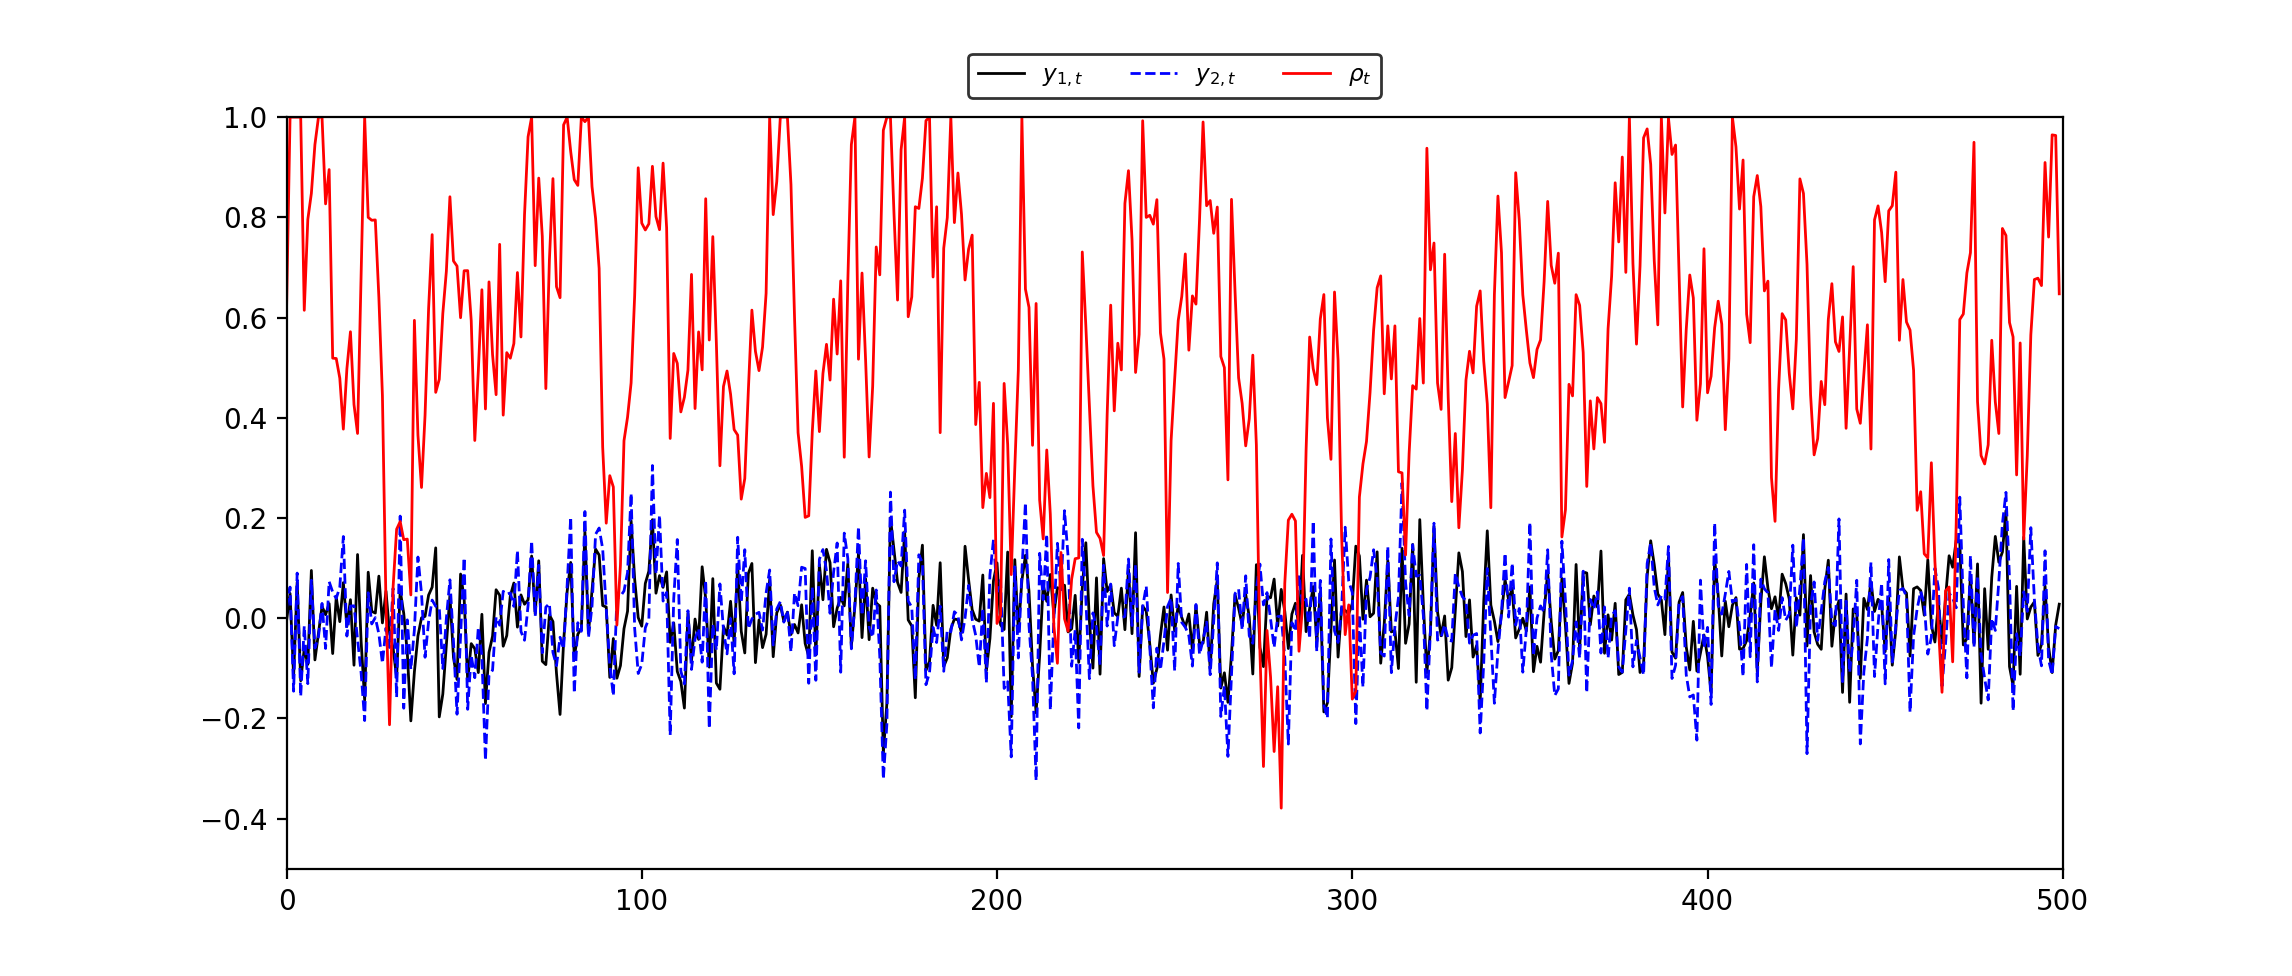
\includegraphics[scale=0.6]{simulation_assetpaths_with_stochastic_correlations.png}
	\caption{Simulated data and time-varying correlations from \eqref{eq:correlation_simulation}.}
	\label{fig:cholesky_simulation}
\end{figure}

\noindent
To assess some of the statistical properties when moving window estimates of correlation coefficient are used as proxies for true correlations in our supervised learning problem, we will denote the estimation uncertainty associated to these coefficients by the width of their $100(1-\eta)\%$ confidence intervals. These confidence intervals are estimated by application of a bootstrap resampling procedure with replacement: For all times $t = \{\Delta t, \Delta t +1, \dots, T\}$, for $\Delta t = \{3, 4, \dots, 100\}$\footnote{Time units for $\Delta_t$ correspond to three to one hundred market days. Given the information on this discrete set of datapoints, it is possible to analyse MSE behaviour.}, a $1000$ samples of size $\Delta t$ have been randomly selected\footnote{A thousand samples is assumed to be a sufficient number of samples to capture the uncertainty around the estimated values.}. For each subsample the correlation coefficient is estimated and, subsequently, the width of the $100(1-\eta)\%$  confidence interval is measured for each coefficient. The parameter $\eta$ is set to $0.01$ in this part of the analysis.    \\ 

\noindent
\textbf{Explain validation mode: sliding or expanding moving window.} \\

\noindent
For the implementation of nearest neighbor and random forest algorithms, we make use of a widely-used machine learning library for the Python programming language: Scikit-learn \citep{ref:Pedregosa2011}. \\ 

\iffalse
\noindent
\textit{Also: We will apply a walk forward validation such that we will retrain our learning algorithm as new data becomes available. Now do we use a Sliding or Expanding window? We need to decide whether the model will be trained on all data it has available or only on the most recent (1000) observations. Its a tough question: shorter windows increase your parameter risk while longer windows increase your model risk. A short data sample increases the chance that your parameter estimates are way off, conditional on your model specification. A longer data sample increases the chance that you are trying to stretch your model to cover more cases than it can accurately represent. If you were certain that the underlying data-generating process was stable, then the more data you have, the better. If not, then maybe not. In our case the data-generating process is stable. This however is not necessarily the case in real financial processes, which will be the focus in multivariate setting. Let's stick with expanding window for now. Especially since Rob Hyndman also  suggests to follow an expanding window procedure.} 
\fi

\section{Moving Window Estimates of Correlation}

\noindent
The accuracy of Pearson and Kendall estimates for time-varying correlation is compared by using mean squared error (MSE) between estimated and actual correlations. The variance of mean squared errors from Pearson estimates in Fig. \ref{fig:mse_pearson_kendall_bootstrap} is approximately 1.78e-3 while that of Kendall is approximately 1.59e-3, i.e. Kendall estimates are slightly less sensitive to the choice of window length compared to Pearson estimates but the difference seems negligible small or might even not be significant. Interestingly, it is observed that Kendall estimates for time-varying correlation have slightly higher MSE values for larger window lengths. A possible explanation for this observation is that the simulated asset returns follow a multivariate normal distribution, i.e. an elliptical distribution. Therefore, it makes sense that a linear correlation coefficient such as Pearson results in lower MSE values for most window lengths. Pearson can get unreliable in the presence of fat-tailed distributions, which is generally a property of real asset return data \citep{ref:Pozzi2012}. It will be interesting to verify whether Kendall is a better choice for approximation of true correlation in the case of real asset return data in Chapter \ref{chap:multivariate_analysis}.  \\

\noindent
Pearson and Kendall moving window estimates of time-varying correlation satisfy the positive semi-definiteness condition in the time-varying correlation matrix $R_t$ for all time $t$ under all choices of window length. Fig. \ref{fig:det_pearson_kendall} presents the obtained minimum determinants of $R_t$ for all choices of window length. In fact, \cite{ref:Pozzi2012} give proves that Pearson and Kendall correlation matrices generally are positive semi-definite matrices.     


\begin{figure}[H]
	\centering
	\begin{subfigure}[b]{0.49 \textwidth}
		\centering 
		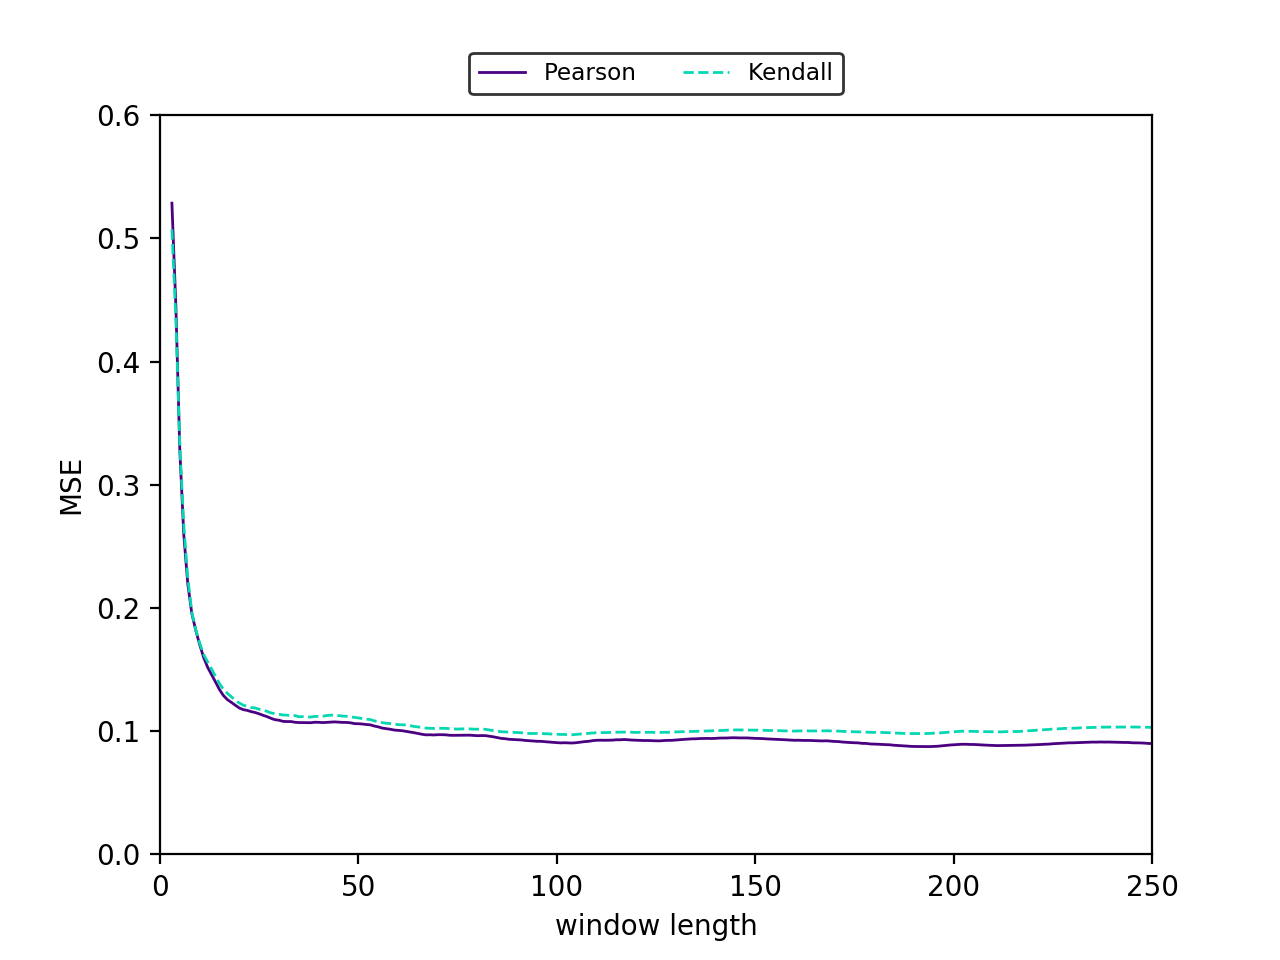
\includegraphics[width=\textwidth]{mse_pearson_kendall.png} 
		\caption{MSE for Pearson and Kendall Moving Window bootstrap estimates.}
		\label{fig:mse_pearson_kendall_bootstrap}
	\end{subfigure}
	\begin{subfigure}[b]{0.49 \textwidth}
		\centering 
		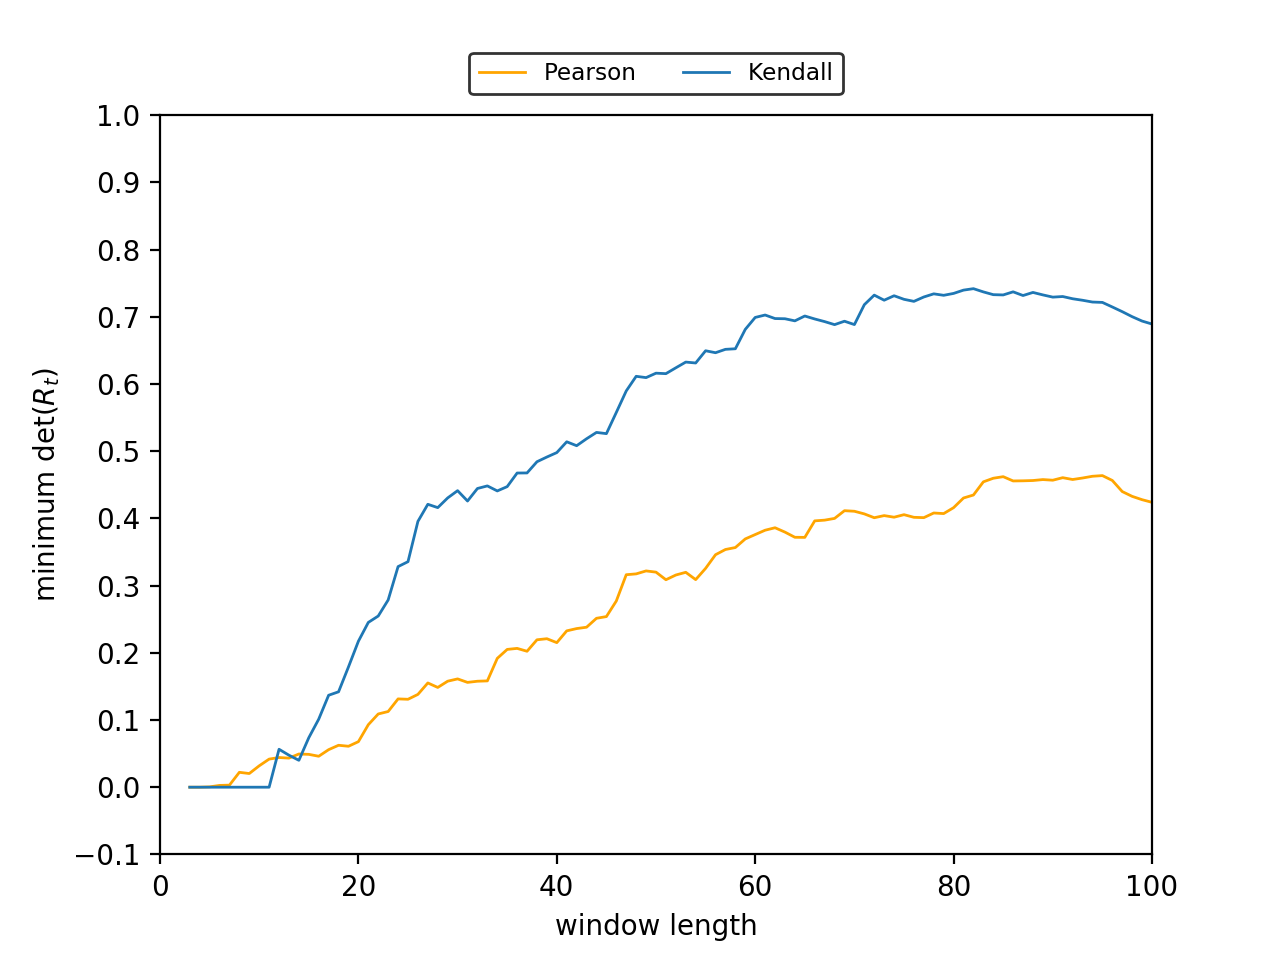
\includegraphics[width=\textwidth]{det_pearson_kendall} 
		\caption{Minimum det($R_t$) from Pearson and Kendall Moving Window bootstrap estimates.}
		\label{fig:det_pearson_kendall}
	\end{subfigure}
	\caption{Comparison MSE and minimum determinants for Pearson and Kendall Moving Window bootstrap estimates\protect\footnotemark.}
	\label{fig:mse_det_pearson_kendall_bootstrap}
\end{figure}


\footnotetext{For Pearson and Kendall correlation approximation using moving window estimates with window sizes 3 through 7 several bootstrapped samples return a standard deviation of zero. This results into NaN values for the associated estimated correlation coefficient as the covariance is divided by zero. These NaN values are excluded for calculation of the mean estimate of Pearson and Kendall correlation coefficient over the test set. Thus, as a result of a smaller number of bootstrapped samples used, estimation of Pearson and Kendall correlation coefficient using moving windows with small window sizes are less robust.} 


\noindent
Fig. \ref{fig:pearson21_bootstrap} and Fig. \ref{fig:kendall21_bootstrap} show that both Pearson moving window estimates and Kendall moving window estimates of correlation change substantially over time indicating the capture of changing correlation levels. Additionally, it is observed that the obtained 99\% confidence intervals around these estimates are rather wide, covering all values in the range $[-1,1]$, which imply that the uncertainty around the estimated values are high \citep{ref:Basturk2016}. \\

\noindent
\textbf{Say something on difference between smoothness/ peaks Pearson/Kendall estimates: potentially that kendall seems less volatile, which may be explained by the fact that Kendall is insensitive to outliers?} \\  


\begin{figure}[H]  % [h] parameter makes sure figures are located at 'this' location.
	\centering
	\begin{subfigure}[b]{0.49 \textwidth} % sum of widths should be less than text width if all one the same line
		\centering 
		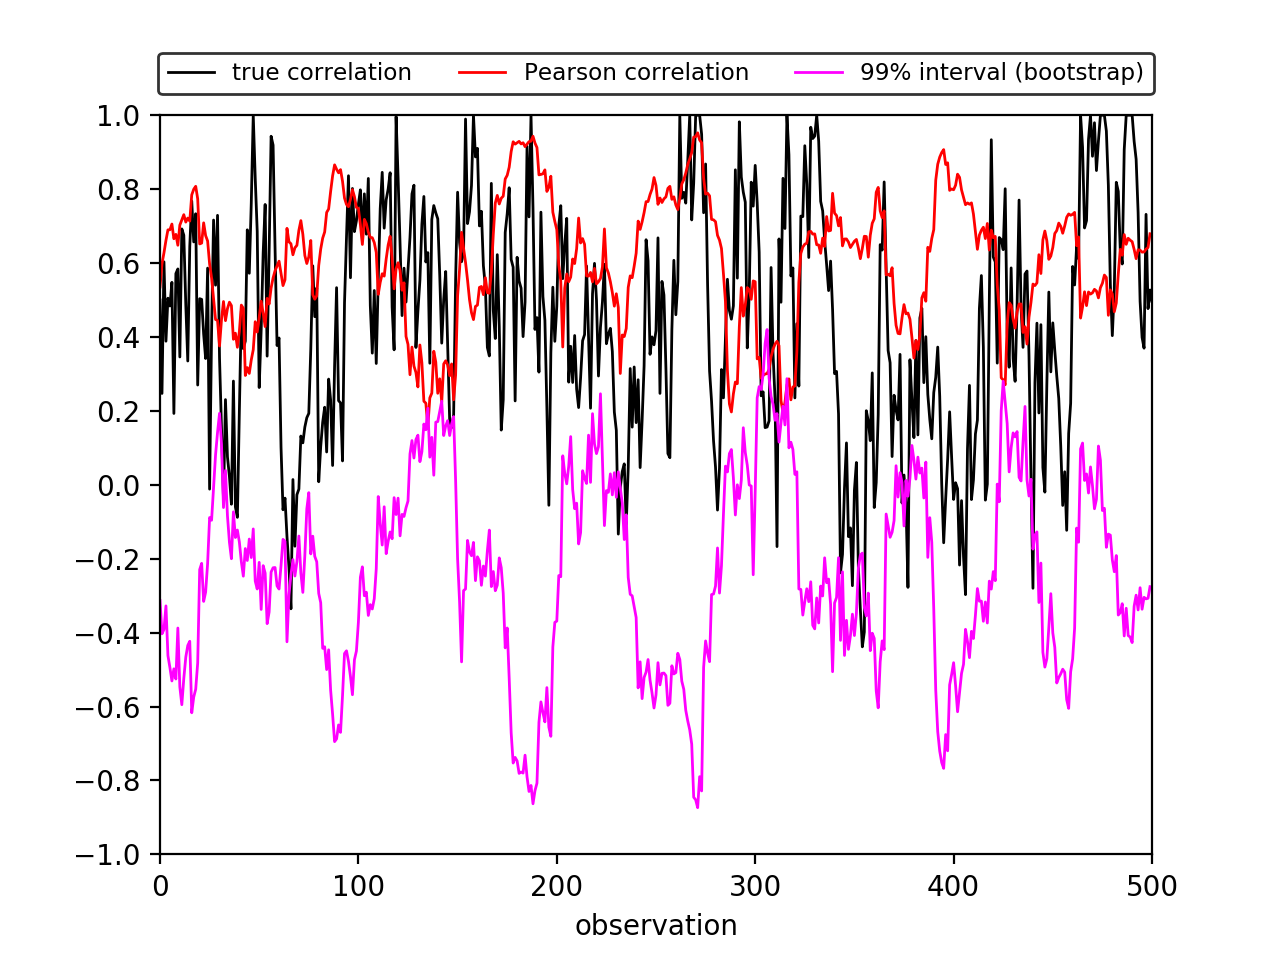
\includegraphics[width=\textwidth]{pearson_21_estimates_bootstrap.png} 
		\caption{Pearson estimates with window size 21.} 		
		\label{fig:pearson21_bootstrap}
	\end{subfigure} 
	\hfill
	\begin{subfigure}[b]{0.49 \textwidth}
		\centering 
		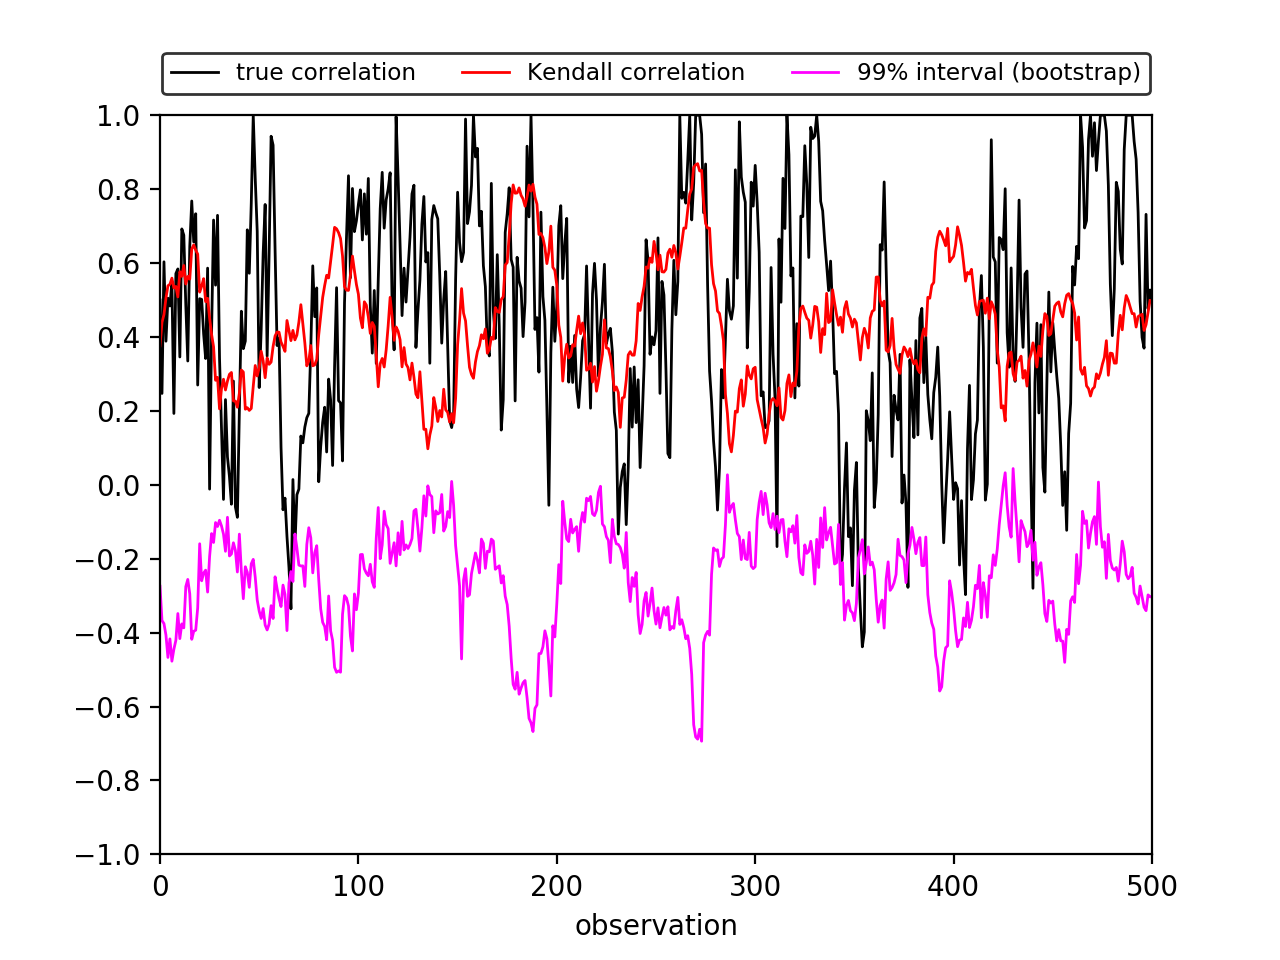
\includegraphics[width=\textwidth]{kendall_21_estimates_bootstrap.png} 
		\caption{Kendall estimates with window size 21.} 		
		\label{fig:kendall21_bootstrap}
	\end{subfigure}
	\hfill
	\begin{subfigure}[b]{0.49 \textwidth} 
		\centering
		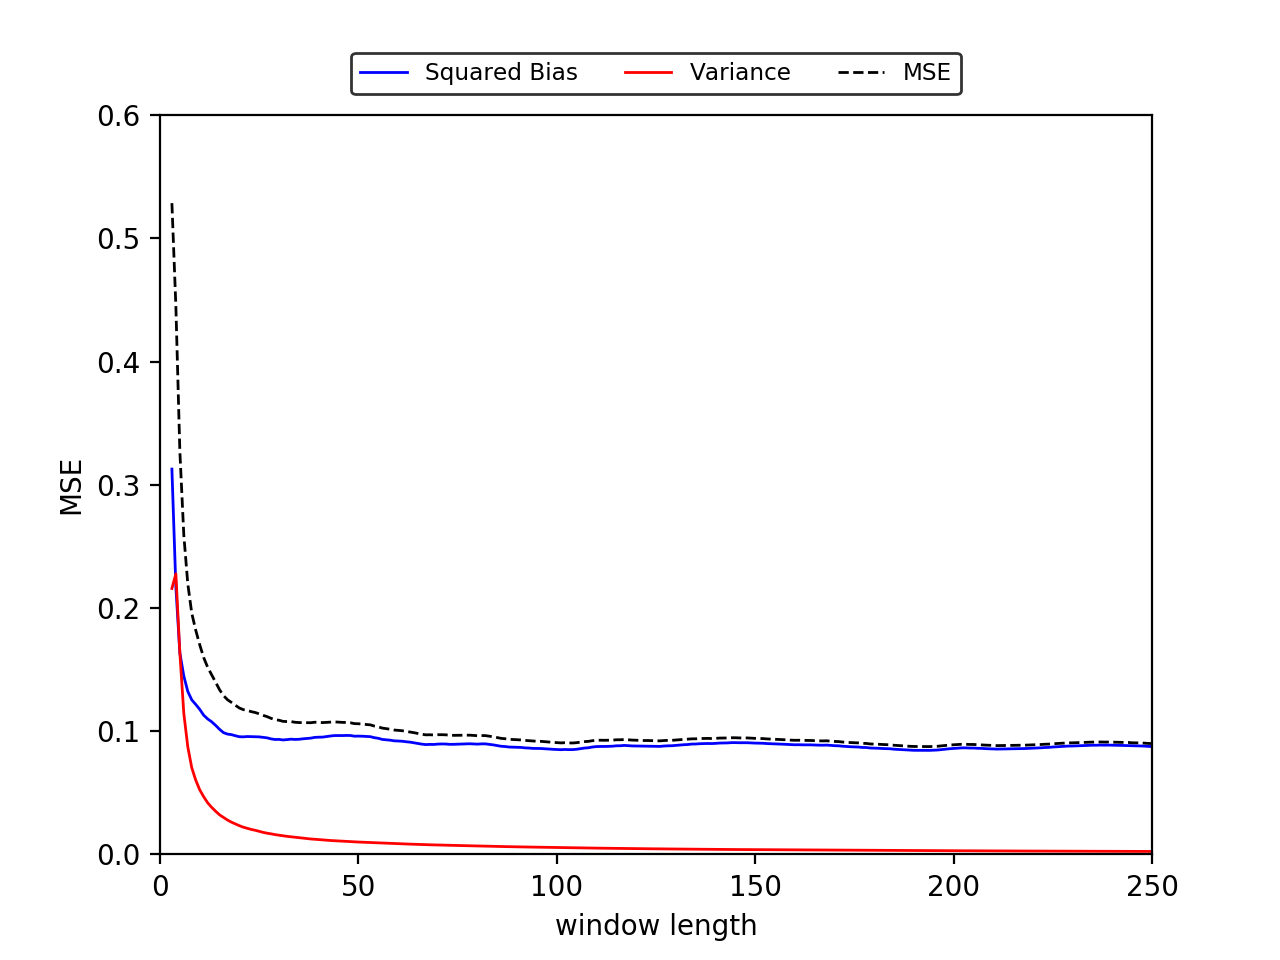
\includegraphics[width=\textwidth]{decom_mse_pearson.png}
		\caption{Bias-variance decomposition for Pearson estimates.}
		\label{fig:decom_mse_pearson}
	\end{subfigure}
	\hfill
	\begin{subfigure}[b]{0.49 \textwidth} 
		\centering
		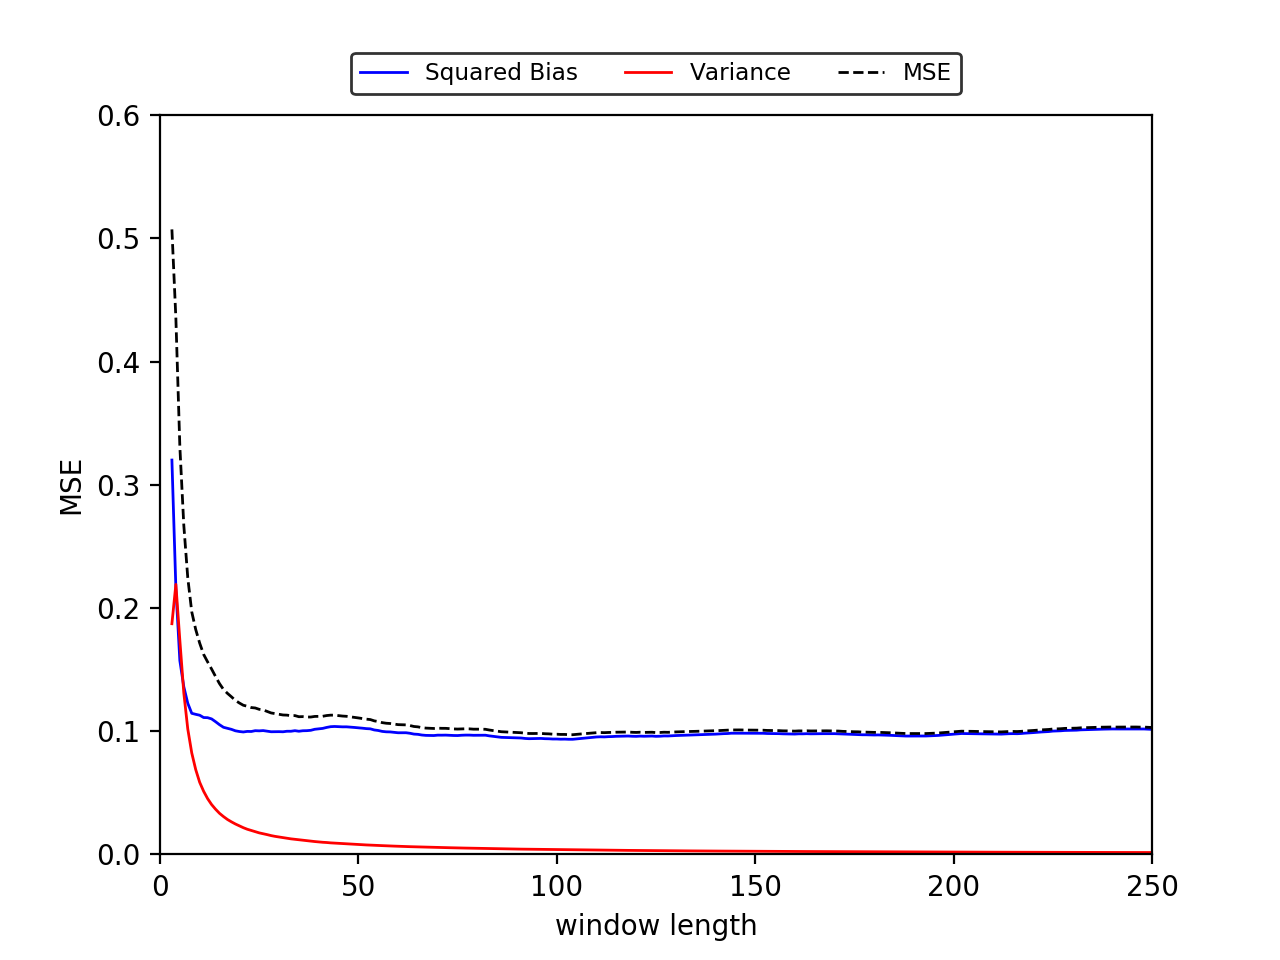
\includegraphics[width=\textwidth]{decom_mse_kendall.png}
		\caption{Bias-variance decomposition for Kendall estimates.}
		\label{fig:decom_mse_kendall}
	\end{subfigure}
	\caption{MSE for Pearson and Kendall Moving Window bootstrap estimates.}
	\label{fig:decom_mse_pearson_kendall_true}
\end{figure}

\noindent
Moreover, Pearson and Kendall estimates are very sensitive to the choice of the window length used for correlation estimates. This is illustrated by the bias-variance decomposition of the mean squared error (MSE) between estimated and actual correlations, shown in Fig. \ref{fig:decom_mse_pearson} and Fig. \ref{fig:decom_mse_kendall}. One can observe an inverse relationship between the choice of window length (i.e. the bootstrap sample size) and value of the variance term in the MSE decomposition. This is explained by the fact that as the bootstrap sample size increases with an increase of the window length, the standard error (i.e. the standard deviation of the sampling distribution) decreases. In other words, as the bootstrap sample size increases, the variability of sampling distribution decreases which would show through smaller 99\% confidence intervals. In these figures it is shown through a decrease in de variance term of the bias-variance decomposition of the mean squared error (MSE) between estimated and actual correlations. \\


\section{Learning with True Correlation for Response Variable and Proxies for Covariates} \label{sec:true_correlation}
"In this section, the input variables of the learning algorithms are approximations of actual (unobserved) correlation. Simulation experiments are used to study the effect using approximations of correlations as the input variables on the learning algorithm results, isolating this effect from the approximations of the response variable, which is illustrated in Section \ref{sec:proxy_correlation}. The simulation study will give insight into the (function) approximation capability of the learning algorithms, particularly in comparison with Pearson and Kendall moving window approximations. This will give us some initial information with respect to possible success of these algorithms in the task of modeling time-varying correlation." \\







%%%%%% NEAREST neighbor TRUE COR %%%%%%%%
\subsection{Nearest Neighbor} \label{sec:knn_true_cor}
In order to obtain time-varying correlations, $\rho_t$, with k-nearest multivariate neighbor algorithm, the data set is defined as in \eqref{eq:dataset}; covariates are constructed from lagged Pearson and Kendall moving window estimates and minimum and maximum log return of the previous time unit, denoted by $min_{i}(r_{i,t-1})$, and $max_{i}(r_{i,t-1})$, respectively.  \\

\subsubsection{Diagnosing the Generalization Error of Nearest Neighbors}
The accuracy of KNN estimates with Pearson and Kendall covariates for time-varying correlation is compared by using mean squared error (MSE) between estimated and actual correlations. MSE from KNN with Pearson and Kendall moving window estimates of correlation for covariates are shown in Fig. \ref{fig:mse_knn5_pearson_kendall_true}. Regardless of the choice of window length, MSE from KNN with Pearson and Kendall covariates are between 0.0939 and 0.1071, and 0.0929 and 0.1071, respectively. The variance of MSE from KNN estimates with Pearson covariates is approximately 6.07e-6 while that of KNN estimates with Kendall covariates is approximately 5.66e-6. KNN thus appears to be insensitive to the choice of window length, regardless whether the set of covariates is constructed from Pearson or Kendall moving window estimates of correlation. KNN's property of insensitivity to the choice of window length is preferred over Pearson and Kendall's property of being highly sensitive to the choice of the window length used for correlation estimates as depicted in Fig. \ref{fig:mse_pearson_kendall_bootstrap}.  \\

\noindent
Moreover, KNN estimates of time-varying correlation where the set of covariates is constructed from Pearson and Kendall moving window estimates and true correlation as response variable, satisfy the positive semi-definiteness condition in the time-varying correlation matrix $R_t$ for all time $t$ under all choices of window length. Fig. \ref{fig:det_knn5_pearson_kendall_true} presents the obtained minimum determinants of $R_t$ for all choices of window length.  
     
\begin{figure}[H]
	\centering
	\begin{subfigure}[b]{0.49 \textwidth} 
		\centering
		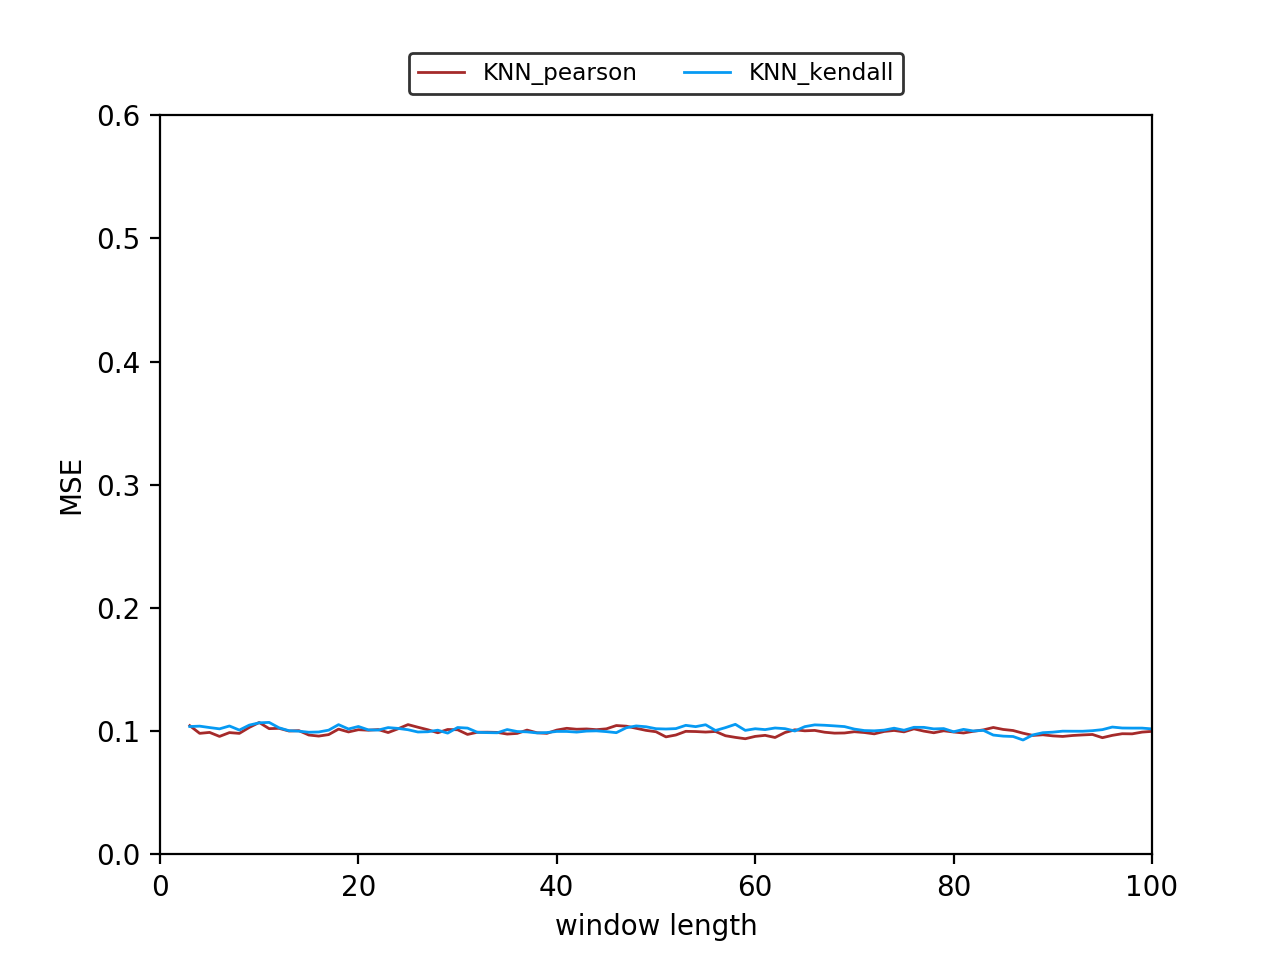
\includegraphics[width=\textwidth]{mse_knn5_pearson_kendall_true.png}
		\caption{MSE for KNN with covariates from Pearson and Kendall and true correlation.}
		\label{fig:mse_knn5_pearson_kendall_true}
	\end{subfigure}
	\hfill
	\begin{subfigure}[b]{0.49 \textwidth} 
		\centering
		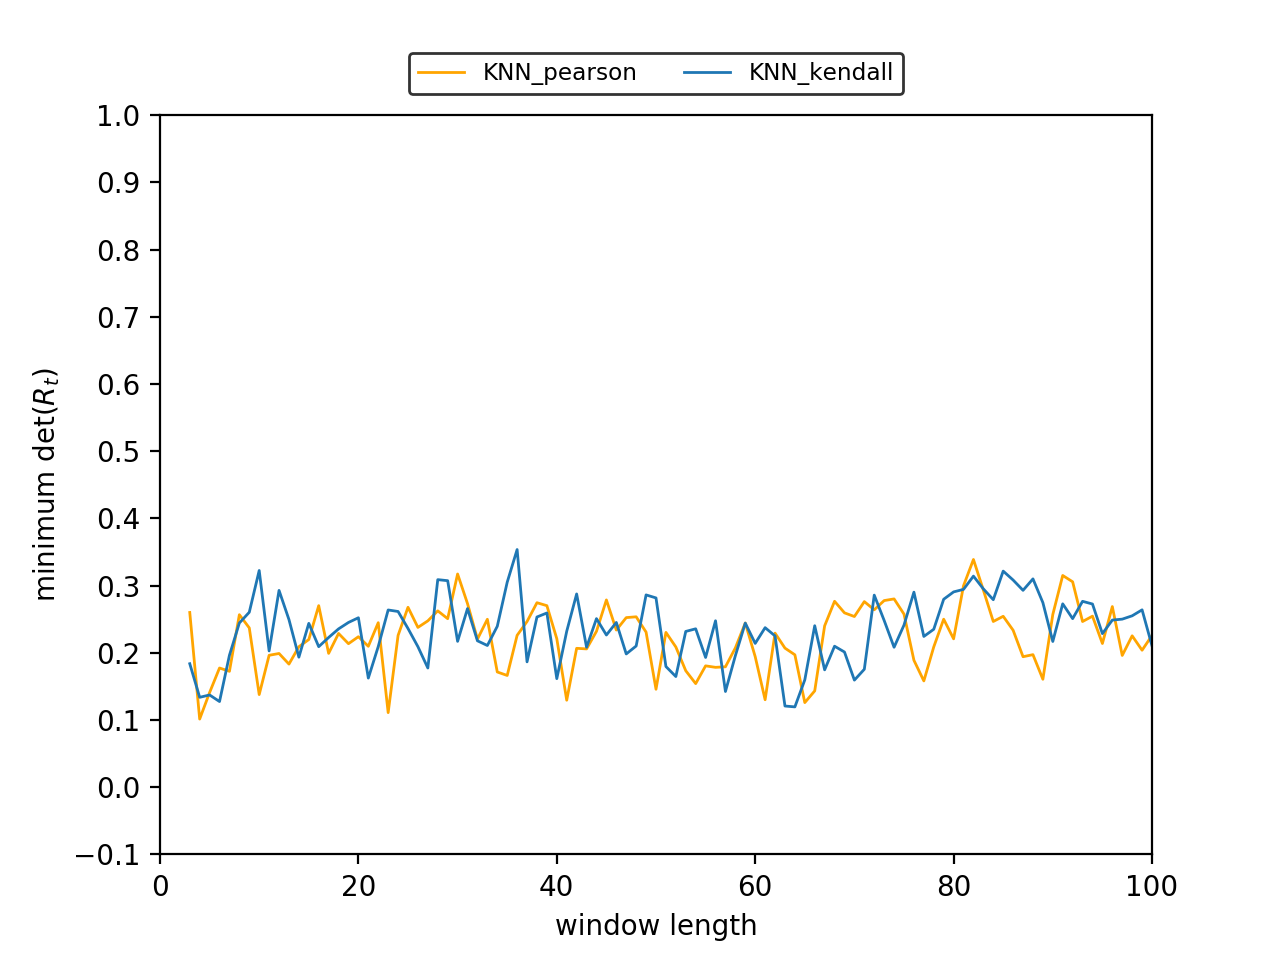
\includegraphics[width=\textwidth]{det_knn5_pearson_kendall_true}
		\caption{Minimum determinants for KNN with covariates from Pearson and Kendall and true correlation.}
		\label{fig:det_knn5_pearson_kendall_true}
	\end{subfigure}
	\caption{Comparison MSE and minimum determinants for KNN(n\_neighbors=5) with covariates from Pearson and Kendall and true correlation.}
	\label{fig:mse_det_knn5_pearson_kendall_true}
\end{figure}



\noindent
From visual inspection of the plots in Fig. \ref{fig:knn_pearson21_bootstrap_true} and Fig. \ref{fig:knn_kendall21_bootstrap_true} it seems that the uncertainty in the time-varying correlation $\rho_t$, which is illustrated by the $99\%$ confidence interval, is smaller for KNN estimates compared to Pearson and Kendall moving window estimates under the same window length of 21. KNN estimates of correlation with number of neighbors equal to 5 are, however, much more volatile. This may be a less desirable result as it is not expected that correlation between assets changes that drastically at each time unit. Rather, correlation is expected to vary gradually over time \citep{ref:Basturk2016}. It is observed though that, as with an increase in the choice of window length for Pearson and Kendall moving window estimates of correlation, an increase in the number of neighbors results in smoother KNN estimates of correlation. \\

\noindent
\textbf{Say something on the bias-variance decomposition of knn with pearson and kendall.} \\

\noindent
The MSE decompositions into bias and variance terms from KNN estimates of correlation are shown in Fig. \ref{fig:decom_mse_knn5_pearson_true} and Fig. \ref{fig:decom_mse_knn5_kendall_true}. These figures indicate that the KNN algorithm is considerably less sensitive to the choice of the window length for smaller window sizes when compared to Pearson and Kendall moving window estimates of correlation. The uncertainty around the estimated correlations appears to be marginally affected by the choice of the window length for all window sizes. This statement is supported by the fact that the variance as a function of the window length behaves like a (more or less) constant red line in these figures.   

\begin{figure}[H]  % [h] parameter makes sure figures are located at 'this' location.
	\centering
	\begin{subfigure}[b]{0.49 \textwidth} % sum of widths should be less than text width if all one the same line
		\centering 
		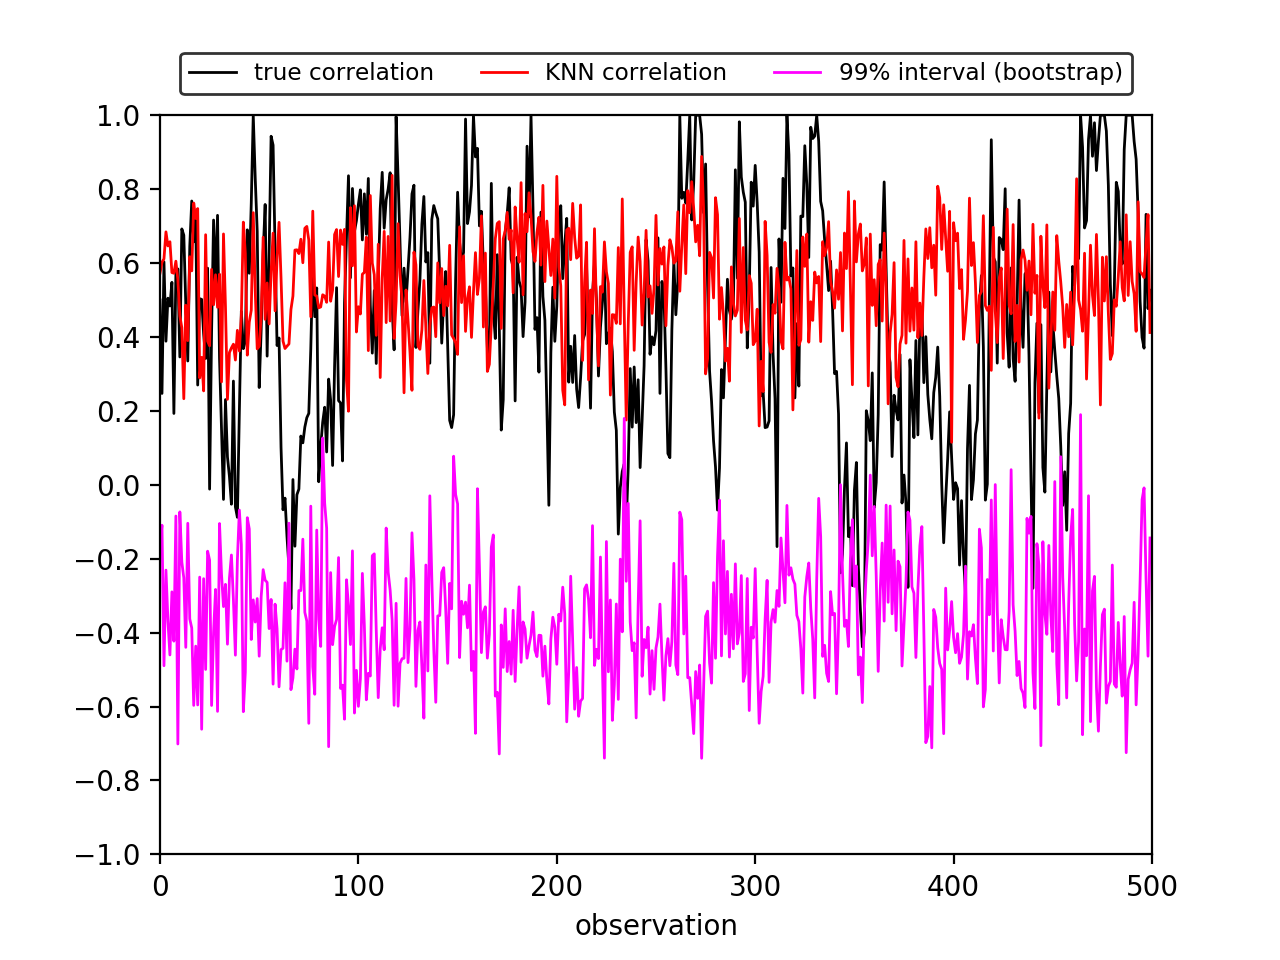
\includegraphics[width=\textwidth]{knn_pearson_21_estimates_bootstrap_true.png} 
		\caption{KNN estimates with window size 21, Pearson as covariate and true correlation.} 	
		\label{fig:knn_pearson21_bootstrap_true}
	\end{subfigure} 
	\hfill	
	\begin{subfigure}[b]{0.49 \textwidth} 
		\centering 
		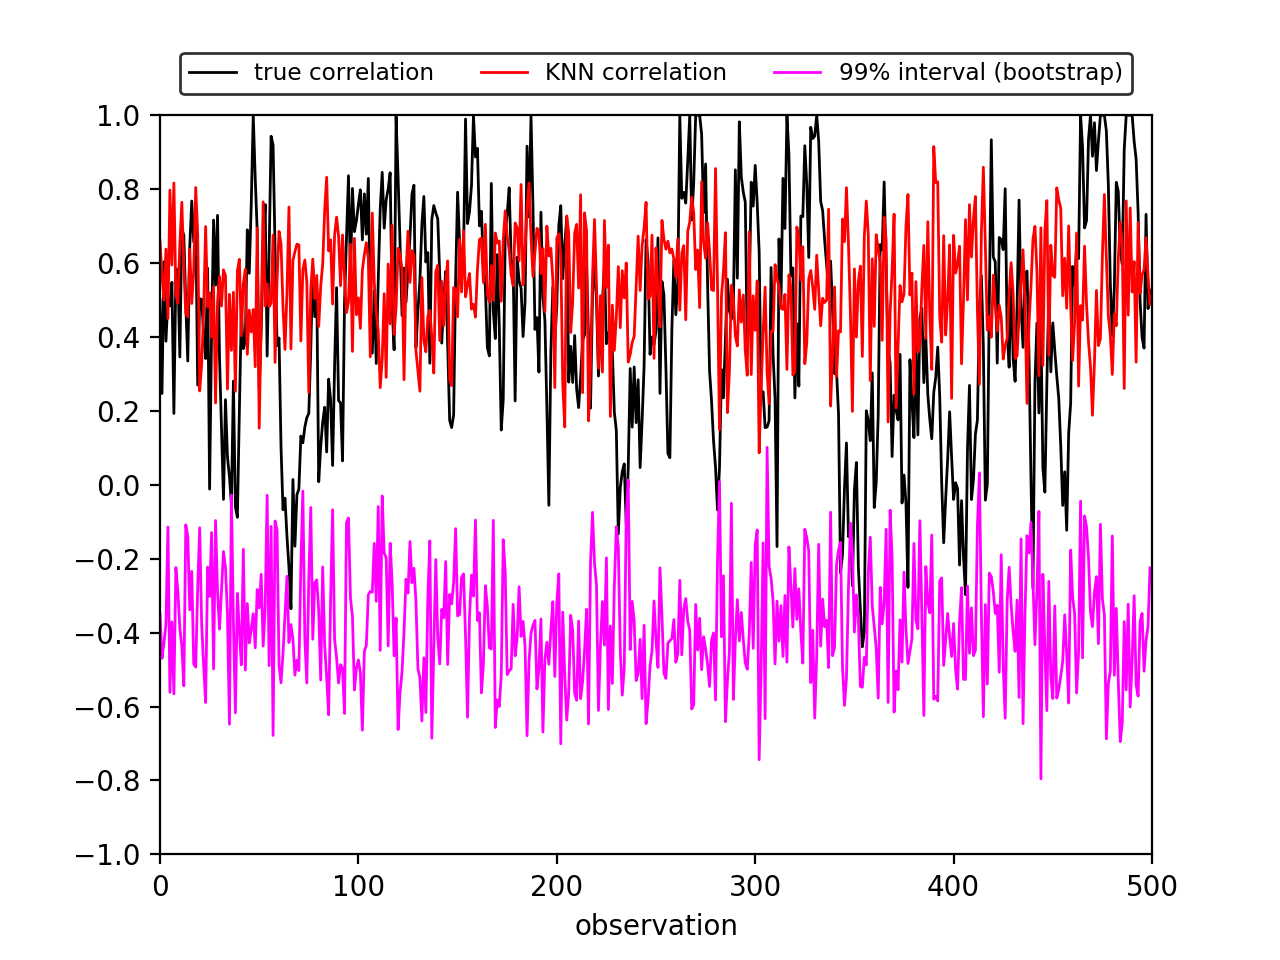
\includegraphics[width=\textwidth]{knn_kendall_21_estimates_bootstrap_true.png} 
		\caption{KNN estimates with window size 21, Kendall as covariate and true correlation.} 
		\label{fig:knn_kendall21_bootstrap_true}
	\end{subfigure} 
	\hfill	
	\begin{subfigure}[b]{0.49 \textwidth}
		\centering 
		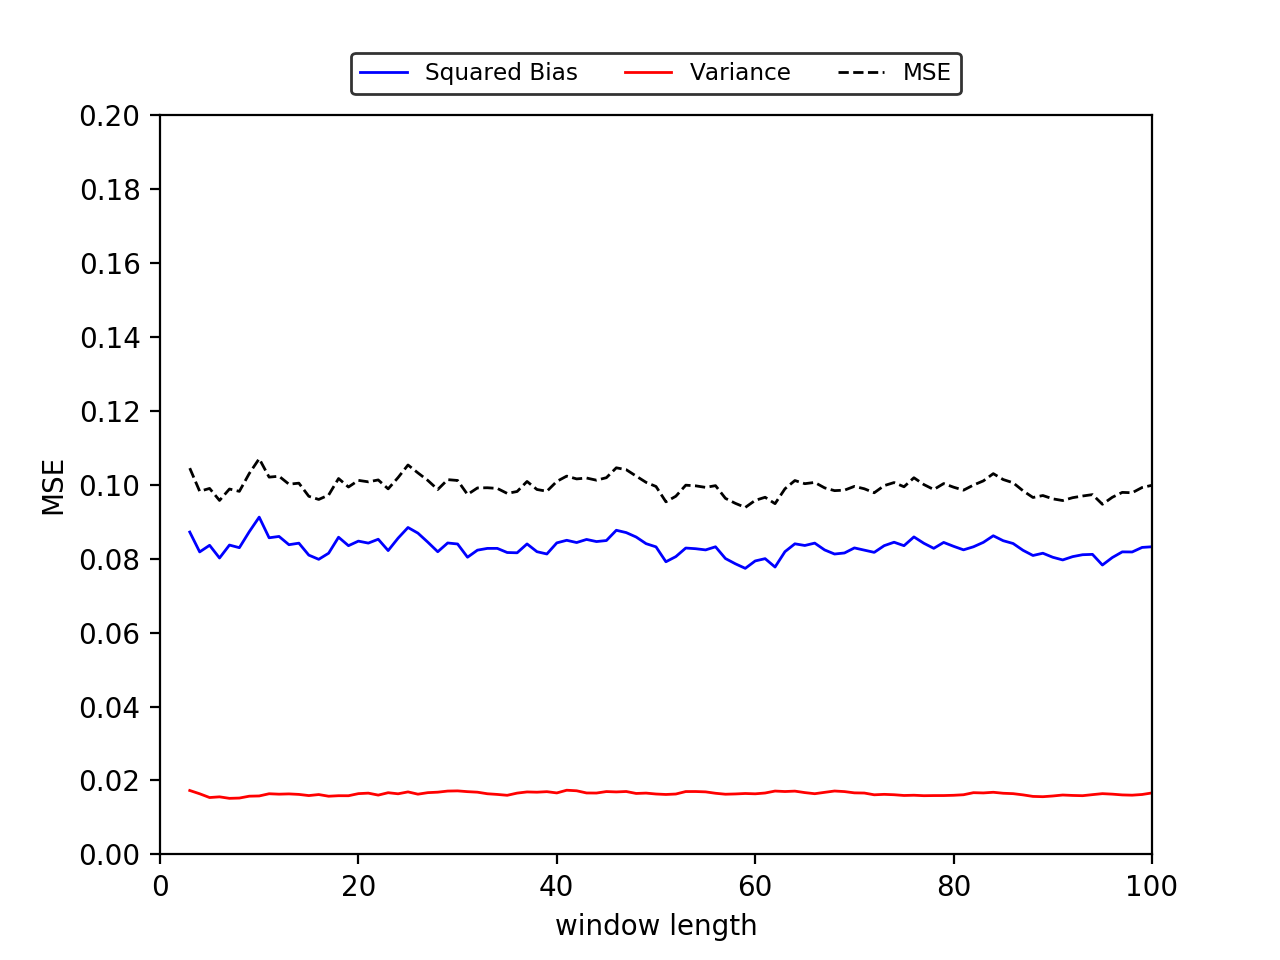
\includegraphics[width=\textwidth]{decom_mse_knn5_pearson_true.png} 
		\caption{Bias-variance decomposition for KNN estimates with Pearson as covariate and true correlation.} 	
		\label{fig:decom_mse_knn5_pearson_true}
	\end{subfigure}
	\hfill  
	\begin{subfigure}[b]{0.49 \textwidth}
		\centering 
		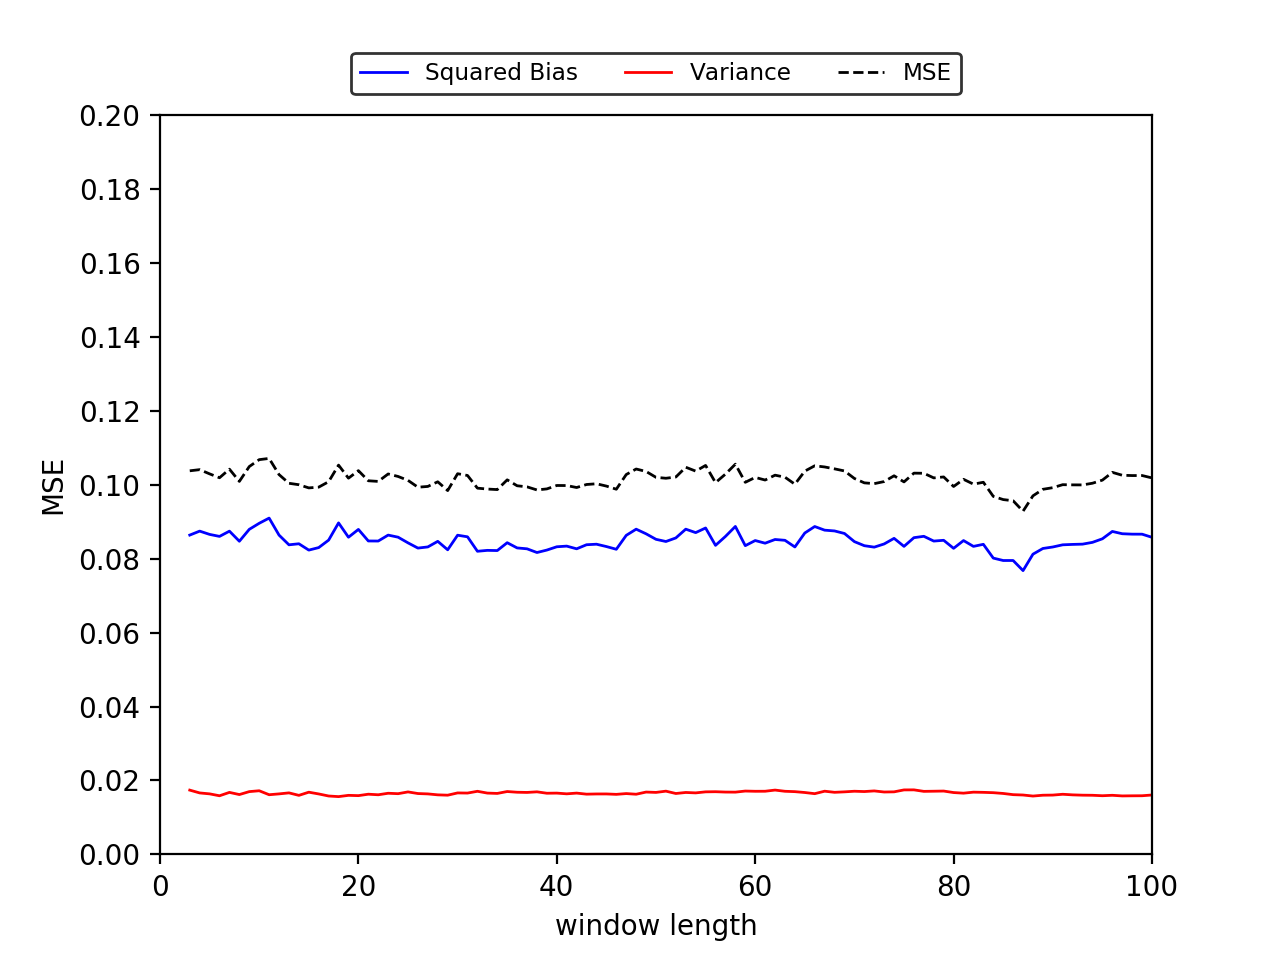
\includegraphics[width=\textwidth]{decom_mse_knn5_kendall_true.png} 
		\caption{Bias-variance decomposition for KNN estimates with Kendall as covariate and true correlation.} 
		\label{fig:decom_mse_knn5_kendall_true}
	\end{subfigure}
	\caption{MSE for KNN estimates with Pearson and Kendall Moving Window bootstrap estimates as covariates and true correlation.}
	\label{fig:decom_mse_knn5_pearson_kendall_true}
\end{figure}

\subsubsection{Alternative Parameterizations of Nearest Neighbor Algorithm}
Fig. \ref{fig:decom_mse_pearson_kendall_true} depicted an inverse relationship between the choice of the window length and the uncertainty around Pearson and Kendall moving window estimates of correlation. The KNN algorithm has a similar property: Simulation results in Tabel \ref{tab:mse_decomp_knn_pearson_kendall_true} show an inverse relationship between the choice of the number of nearest neighbors used in the estimation of correlations and the uncertainty around the estimated correlations, regardless whether Pearson or Kendall estimates are used for defining the set of covariates. It is clearly observed that an increase in the number of neighbors $k$ results in a decrease of the variance, and conversely. This observation is in line with our discussion on MSE decomposition for the KNN algorithm and Eq. \eqref{eq:mse_decomposition_knn} from Section \ref{sec:mse_decompose}. Additionally, it was stated that the higher the value of $k$, the lower the model complexity and, as such, the squared bias tends to increase with an increase in $k$. However, simulation results depicted in Tabel \ref{tab:mse_decomp_knn_pearson_kendall_true} indicate no increase in squared bias with an increase in $k$ up to $k=800$. The first increase in squared bias is observed when the number of neighbors is approximately 900. For all $k$ smaller than 900 a decrease in squared bias is observed with an increase in $k$. This statement is more clearly shown through a geometrical representation of the MSE decomposition as a function of the number of neighbors for $k \in \{5, 10, 25, 50, 100\}$ in Fig. \ref{fig:knn5_pearson_kendall_sens_analysis_true}. \\  




%% TABLE
\begin{table}[H]
\centering
\captionsetup[subtable]{position=below}
%\captionsetup[table]{position=below}
\begin{subtable}{0.49\linewidth}
\centering
\begin{tabular}{r  c  c  c} 
\toprule
\multicolumn{1}{ r }{\textbf{k}} &
\multicolumn{1}{ c }{\textbf{Squared Bias}} &
\multicolumn{1}{ c }{\textbf{Variance}} &
\multicolumn{1}{ c }{\textbf{MSE}} \\
\midrule 

5                                     & 0.0913                         & 0.0158                & 0.1071     \\
10                                   & 0.0831                         & 0.0087                & 0.0917     \\
25                                   & 0.0785 	                    & 0.0037                & 0.0821     \\
50                                   & 0.0781                         & 0.0018                & 0.0799     \\
100                                 & 0.0785                         & 9.23e-4               & 0.0794      \\
200                                 & 0.0776                         & 4.62e-4               & 0.0781      \\
400                                 & 0.0768                         & 2.31e-4               & 0.0770      \\
600                                 & 0.0757                         & 1.55e-4               & 0.0759     \\
800                                 & 0.0756                         & 1.18e-4               & 0.0757      \\
900				     & 0.0761			   & 1.06e-4              & 0.0760      \\
1000                               & 0.0767                         &  9.70e-5              & 0.0768     \\ [1ex]
\bottomrule
\end{tabular}
\caption{MSE for KNN estimates with window size 10, Pearson as covariate and true correlation.}
\label{tab:mse_decomp_knn_pearson_true}
\end{subtable}
\hfill
\begin{subtable}{0.49\linewidth}
\centering
\begin{tabular}{r  c  c  c} 
\toprule
\multicolumn{1}{ r }{\textbf{k}} &
\multicolumn{1}{ c }{\textbf{Squared Bias}} &
\multicolumn{1}{ c }{\textbf{Variance}} &
\multicolumn{1}{ c }{\textbf{MSE}} \\
\midrule 

5                                     & 0.0896                         &  0.0172               & 0.1068   \\
10                                   & 0.0828                         & 0.0092                & 0.0920   \\
25                                   & 0.0764	                   & 0.0038                & 0.0802    \\
50                                   &  0.0749                        & 0.0019               & 0.0769    \\
100                                 & 0.0749                         & 9.47e-4               & 0.0759    \\
200                                 &  0.0753                        & 4.69e-4              & 0.0757    \\
400                                 &  0.0750                        & 2.37e-4              & 0.0752    \\
600                                 & 0.0749                         & 1.59e-4             & 0.0750     \\
800                                 &   0.0750                       & 1.21e-4             & 0.0751     \\
900				     &  0.0757			   & 1.08e-4             & 0.0758     \\
1000                               &  0.0763                        & 9.80e-5             & 0.0764     \\  [1ex]
\bottomrule
\end{tabular}
\caption{MSE for KNN estimates with window size 10, Kendall as covariate and true correlation.}
\label{tab:mse_decomp_knn_kendall_true}
\end{subtable}
\caption{Mean Squared Error (MSE) decomposition as a function of the number of neighbors (k) for KNN with proxy for covariates and true correlation.}
\label{tab:mse_decomp_knn_pearson_kendall_true}
\end{table}

\noindent
Fig. \ref{fig:knn5_pearson_sens_analysis_true} and Fig. \ref{fig:knn5_kendall_sens_analysis_true}  depict geometrical representations of the simulation results for KNN estimates with Pearson and Kendall covariates (and true correlation), respectively. The MSE decomposition as a function of the number of neighbors for $k \in \{5, 10, 25, 50, 100\}$ clearly shows a decrease in the squared bias with an increase in $k$. Given
Eq. \eqref{eq:mse_decomposition_knn} and our discussion from Section \ref{sec:mse_decompose} one might have expected an increase in squared bias with an increase in $k$. A possible explanation for the behaviour depicted in Fig. \ref{fig:knn5_pearson_kendall_sens_analysis_true} may be that up to some $k$, an increase in $k$ implies additional neighbors containing informational value are used for the estimation of time-varying correlations. Logically, the inclusion of additional neighbors containing informational value results into more accurate estimates of correlation, i.e. a decrease in squared bias. As of some $k$, additional neighbors only add noise to the estimation process which results into increased squared bias.    

\begin{figure}[H]  % [h] parameter makes sure figures are located at 'this' location.
	\centering
	\begin{subfigure}[b]{0.49 \textwidth} % sum of widths should be less than text width if all one the same line
		\centering 
		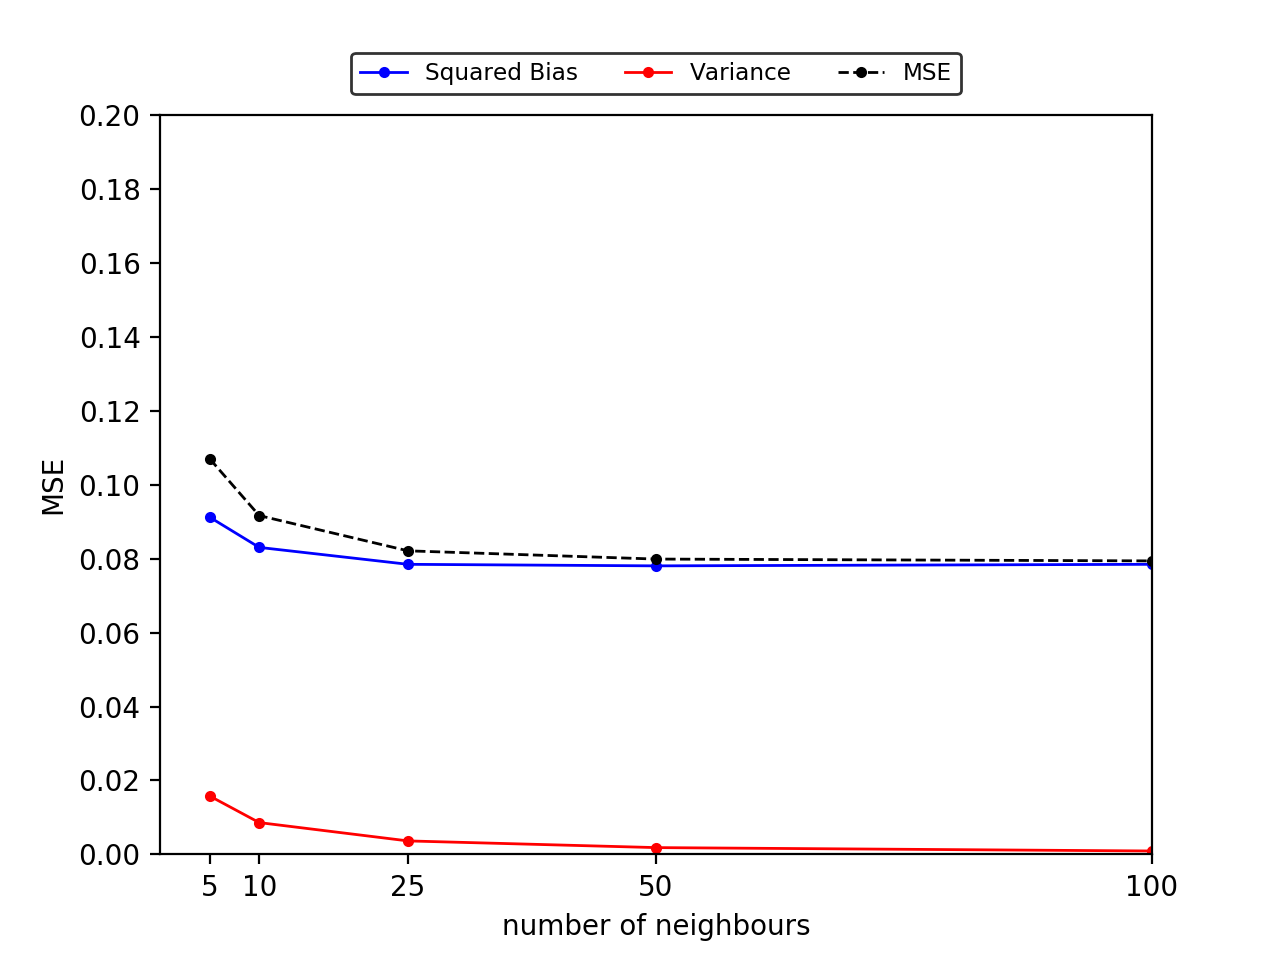
\includegraphics[width=\textwidth]{sens_analysis_mse_knn_pearson_true.png} 
		\caption{KNN estimates with window size 10, Pearson as covariate and true correlation.}
		\label{fig:knn5_pearson_sens_analysis_true}
	\end{subfigure} 
	\hfill	
	\begin{subfigure}[b]{0.49 \textwidth} 
		\centering 
		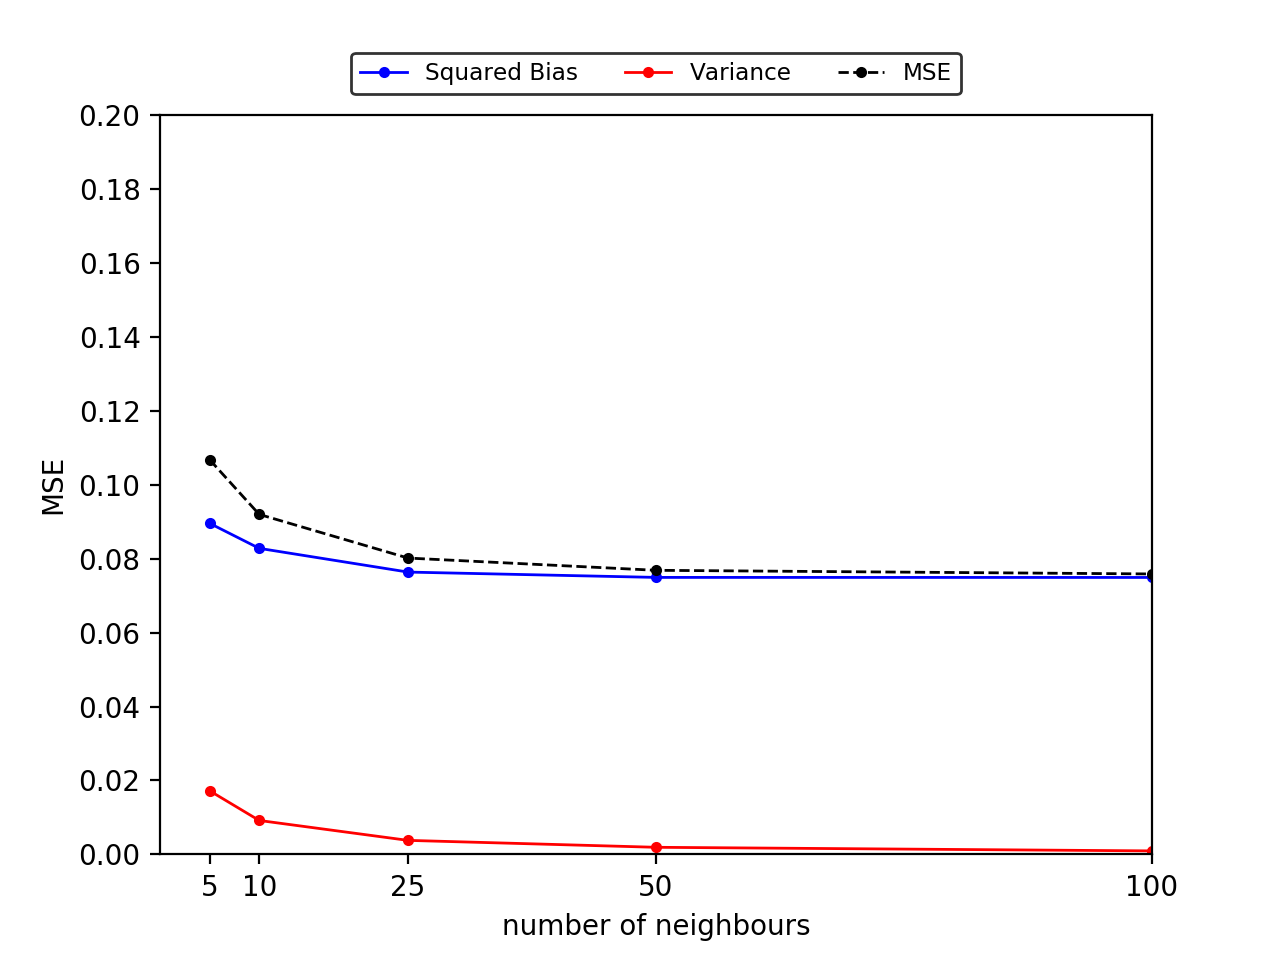
\includegraphics[width=\textwidth]{sens_analysis_mse_knn_kendall_true.png} 
		\caption{KNN estimates window size 10, Kendall as covariate and true correlation.} 
		\label{fig:knn5_kendall_sens_analysis_true}
	\end{subfigure} 
	\caption{MSE as function of number of neighbors for KNN estimates with Pearson and Kendall as covariates and true correlation.}
	\label{fig:knn5_pearson_kendall_sens_analysis_true}
\end{figure}

\noindent
Next, two more interesting parameterizations of the KNN learning algorithm are analysed. In both parameterizations, the set of neighbors used for point estimation of time-varying correlation is defined as the entire training set. However, in the first parameterizations, the KNN algorithm uses an uniformly weighted average of correlations, i.e. each of the neighbors contributing equally to the point estimate of time-varying correlation. In the second parameterizations, the KNN algorithm uses an inverse distance weighted average of correlations, as defined in \eqref{eq:IDWfunction}. The MSE decomposition of both parameterizations with Pearson covariates and true correlation is depicted in Fig. \ref{fig:decom_mse_knn_len_train_IDW_pearson_kendall_true}. It is clear that the variance terms becomes negligible small in case the set of neighbors used for point estimation of time-varying correlation is defined as the entire training set, regardless of the weighting function. The red line of the variance is barely observable in the bottom of Fig. \ref{fig:decom_mse_knn_len_train_pearson_true} and Fig. \ref{fig:decom_mse_knn_IDW_pearson_true}. This is in line with results depicted in Tabel \ref{tab:mse_decomp_knn_pearson_kendall_true} where the value of the variance term is negligible small for $k=1000$, regardless whether the set of covariates is constructed from Pearson or Kendall moving window estimates of correlation.    \\      

\noindent
\textbf{Comment on Figures containing correlation dynamics and state that it resembles assuming constant correlation when number of neighbours equals the trianing set, which is the exact concept we are trying to improve on with time-varying correlations. With an inverse distance weighting we do capture time-varying dynamics of correlation. Low volatility and smoothness and very small variance; properties that are preferred. Maybe too low volatility? Fine, then optimize over $k$, which is only one parameter and could be done by optimizing over some grid of values.}

\begin{figure}[H]  % [h] parameter makes sure figures are located at 'this' location.
	\centering
	\begin{subfigure}[b]{0.49 \textwidth}
		\centering 
		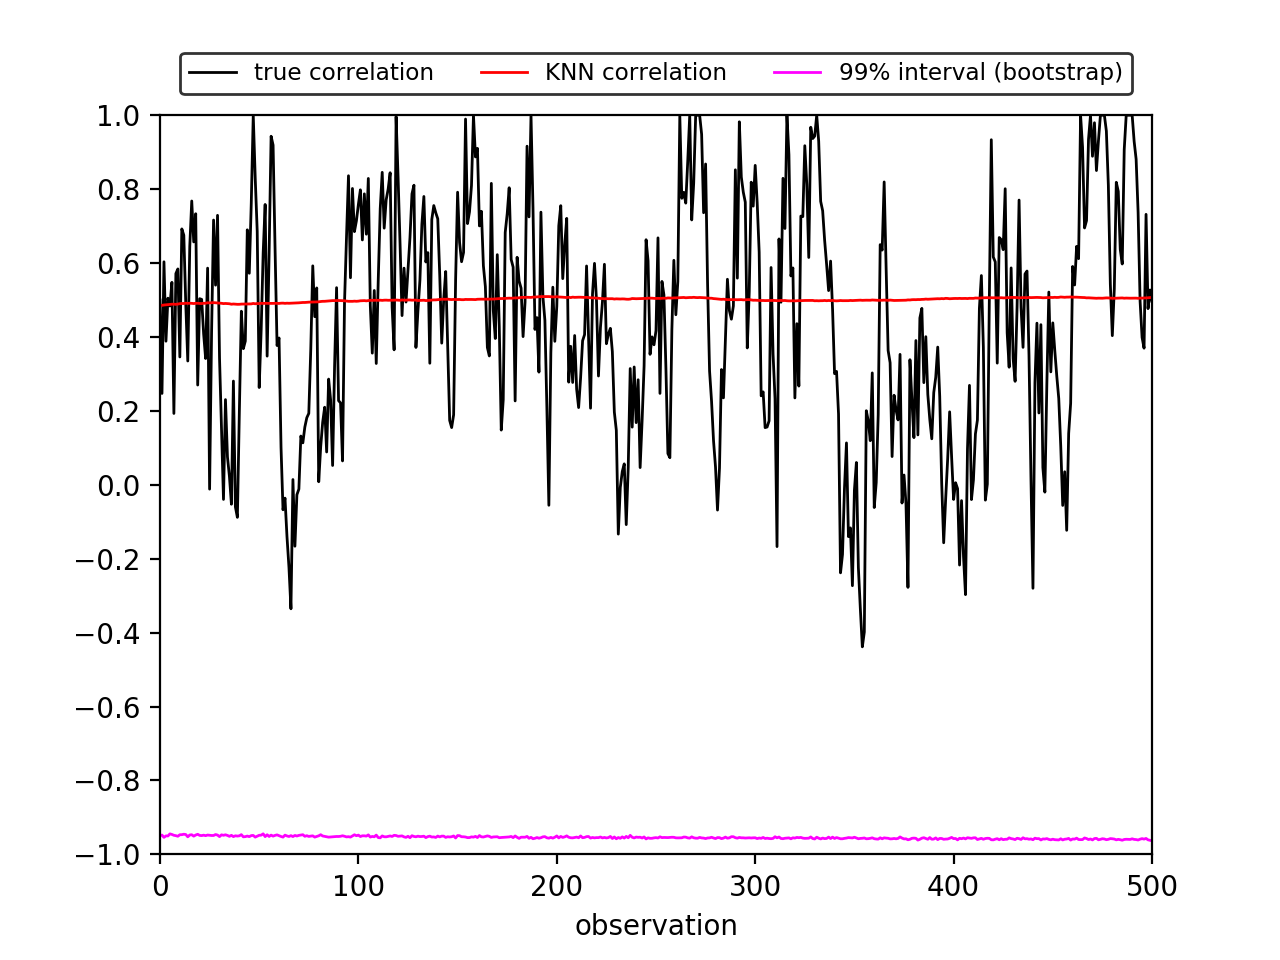
\includegraphics[width=\textwidth]{knn_pearson_21_len_train_estimates_bootstrap_true.png} 
		\caption{KNN estimates as uniformly weighted averages, with window size 21 and Pearson covariates.} 	
		\label{fig:knn_pearson21_len_train_bootstrap_true}
	\end{subfigure}
	\hfill  
	\begin{subfigure}[b]{0.49 \textwidth}
		\centering 
		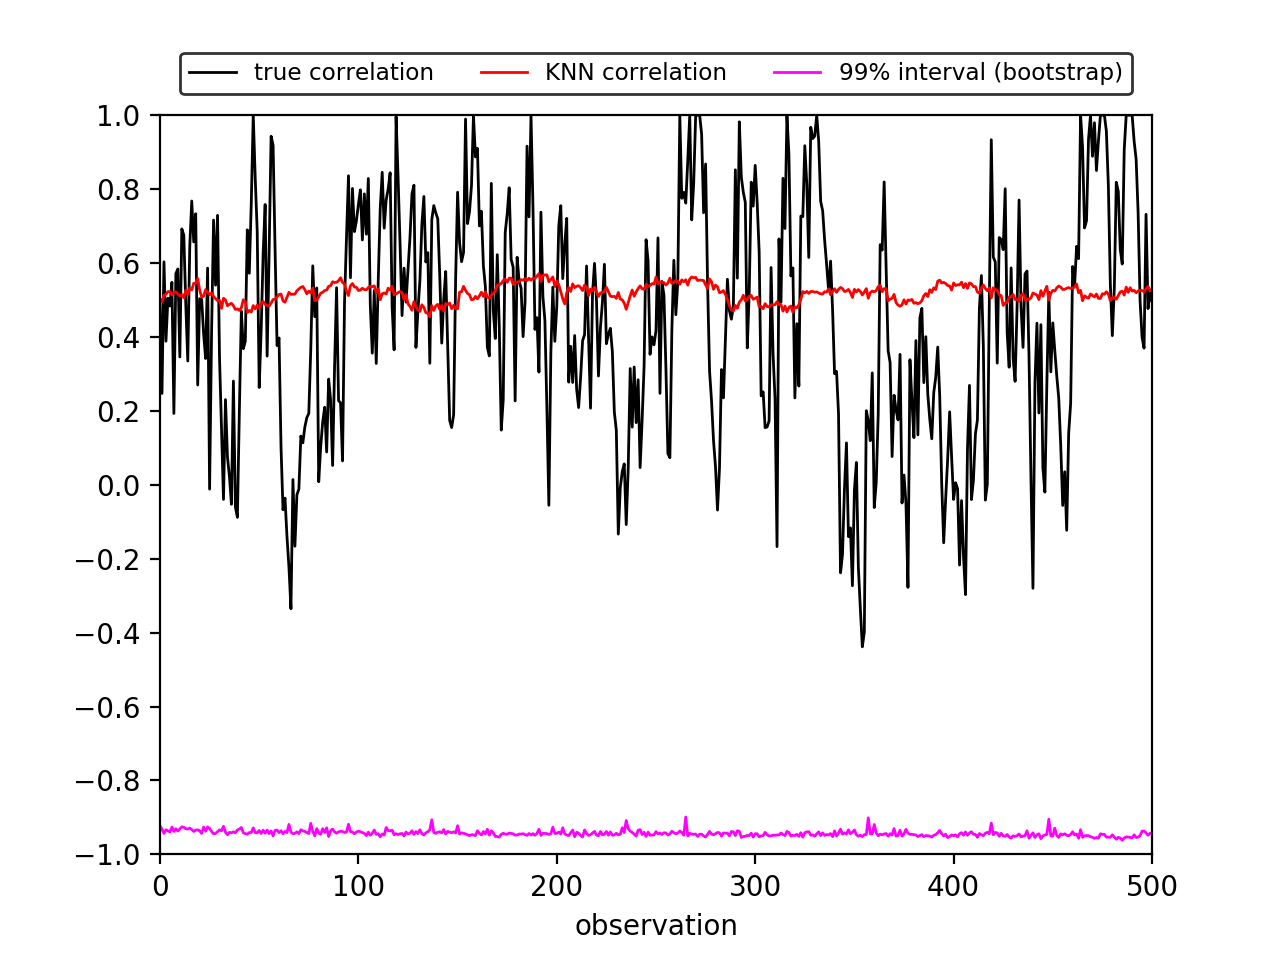
\includegraphics[width=\textwidth]{knn_pearson_21_IDW_estimates_bootstrap_true.png} 
		\caption{KNN estimates as inverse distance weighted averages, with window size 21 and Pearson covariates.} 
		\label{fig:knn_pearson21_IDW_bootstrap_true}
	\end{subfigure}

	\begin{subfigure}[b]{0.49 \textwidth}
		\centering 
		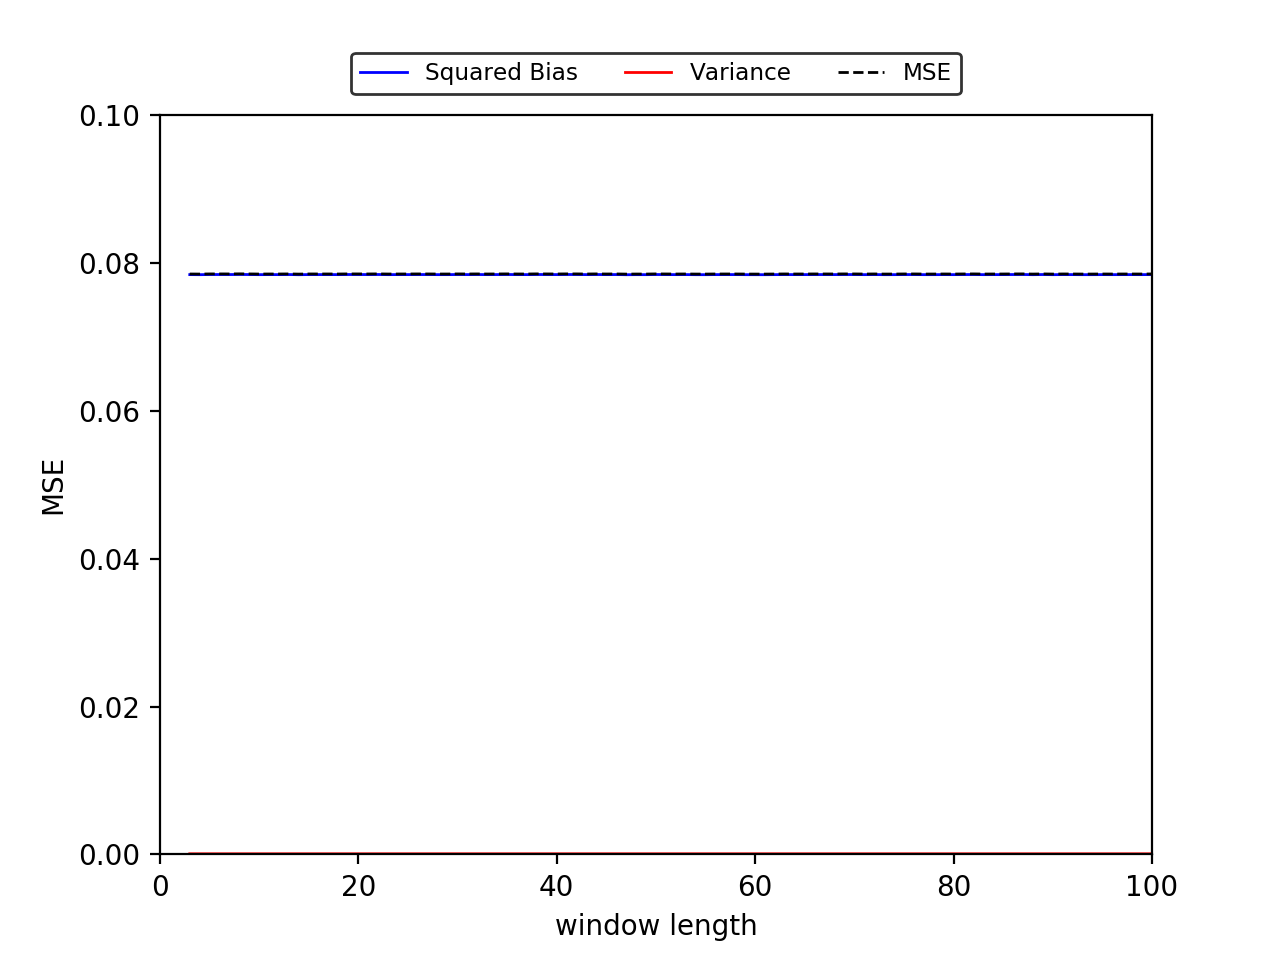
\includegraphics[width=\textwidth]{decom_mse_knn_len_train_pearson_true.png} 
		\caption{Bias-variance decomposition for KNN estimates constructed from uniformly weighted averages.} 	
		\label{fig:decom_mse_knn_len_train_pearson_true}
	\end{subfigure}
	\hfill  
	\begin{subfigure}[b]{0.49 \textwidth}
		\centering 
		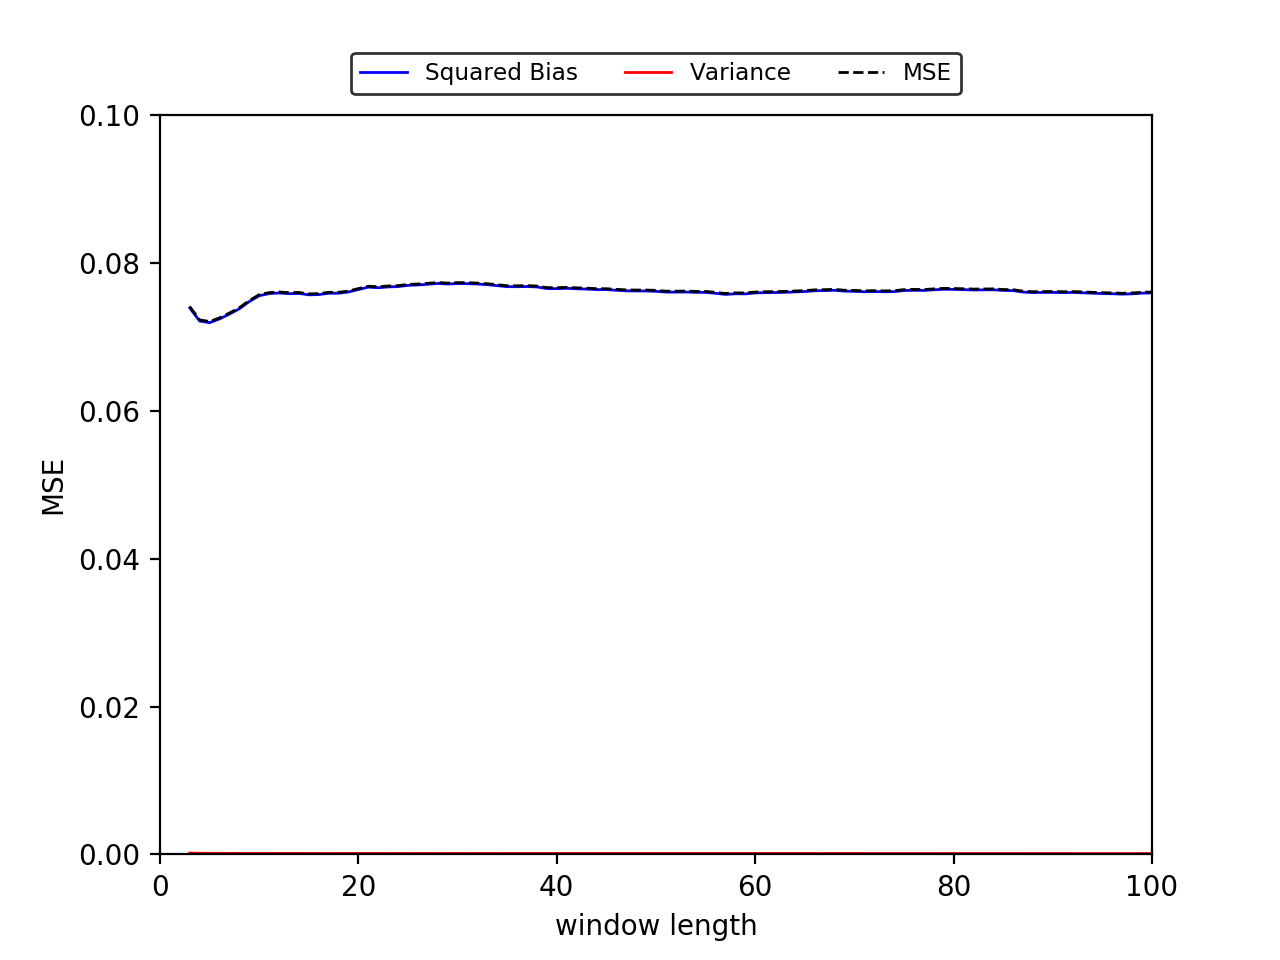
\includegraphics[width=\textwidth]{decom_mse_knn_IDW_pearson_true.png} 
		\caption{Bias-variance decomposition for KNN estimates constructed from inverse distance weighted averages.} 
		\label{fig:decom_mse_knn_IDW_pearson_true}
	\end{subfigure}
	\caption{MSE for KNN estimates with different weighting functions, Pearson Moving Window bootstrap estimates as covariates and true correlation.}
	\label{fig:decom_mse_knn_len_train_IDW_pearson_kendall_true}
\end{figure}

\noindent
The accuracy of the two different parameterizations is compared by using mean squared error (MSE) between estimated and actual correlations. In Fig. \ref{fig:decom_mse_knn_len_train_pearson_true}, MSE from KNN with an uniform weighting function is approximately 0.0785, regardless of the choice of window length and whether Pearson or Kendall moving window estimates are use for constructing the set of covariates. In Fig. \ref{fig:decom_mse_knn_IDW_pearson_true} MSE from KNN with an inverse distance weighting function is approximately between 0.0721 and 0.0774, and between 0.0727 and 0.0771 when Pearson and Kendall moving window estimates are used as covariates, respectively. This implies that slightly lower MSE values are obtained with an inverse distance weighting function as opposed to an uniform weighting function, which is line with our discussion from Section \ref{sec:knn}. It makes sense to have training instances with a higher amount of proximity to the test instance contribute more to the value of the response variable than training instances with a lower amount of proximity to the test instance. Moreover, Fig. \ref{fig:decom_mse_knn_len_train_IDW_pearson_kendall_true} shows that both parameterizations are insensitive to the choice of window length, regardless of the weighting function and choice of covariate. In fact, the variance of MSE from KNN with uniform weighting function and inverse distance weighting function are 5.00e-11 and 8.55e-7, respectively, i.e. hardly significantly different from one another. \\

\noindent
The alternative parameterizations of the KNN algorithm with approximated covariates and response variable also satisfy the positive semi-definiteness condition in the time-varying correlation matrix $R_t$ for all time $t$ under all choices of window length in the interval [0, 100]. Fig. \ref{fig:det_knn_IDW_pearson_kendall_true.png} presents the obtained minimum determinants of $R_t$ for all choices of window length under an inverse distance weighting function\footnote{Usage of an uniform distance weighting function results into an approximately constant minimum determinant of 0.74, for both Pearson and Kendall approximations.}.  \\ 

\noindent
This section is concluded with a comparison of the function approximation capabilities of the KNN algorithm and Pearson and Kendall moving window estimates. The comparison is based on MSE between estimated and actual correlations. Fig. \ref{fig:mse_knn5_idw_pearson_kendall_true} shows MSE from KNN with default parameterizations, i.e. number of neighbors equals 5, an alternative parameterizations with an inverse distance weighting function as well as Pearson and Kendall moving window estimates of time-varying correlations. According to MSE, parameterizations of the KNN algorithm where the number of neighbors is 5 or 10 perform better than those of Pearson and Kendall moving window estimates for small window sizes. Moreover, parameterizations of the KNN algorithm with an alternative distance weighting function and where the entire training data set is used for estimating correlation result in significantly smaller MSE compared to Pearson and Kendall moving window estimates for all window sizes. In fact, the simulation study shows that the KNN algorithm outperforms Pearson and Kendall moving window estimates of correlation for all window sizes when the number of neighbors $k \in \{25, 50, 100\}$ in addition to both alternative parameterizations. Finally, the variance of MSE from KNN estimates with default parameterizations and with an inverse distance weighting function in Fig. \ref{fig:mse_knn5_idw_pearson_kendall_true} are 6.07e-6 and 8.55e-7, respectively, while that of Pearson and Kendall moving window estimates are 0.0040 and 0.0037, respectively. \\


\begin{figure}[H]  % [h] parameter makes sure figures are located at 'this' location.
	\centering
	\begin{subfigure}[b]{0.49 \textwidth}
		\centering 
		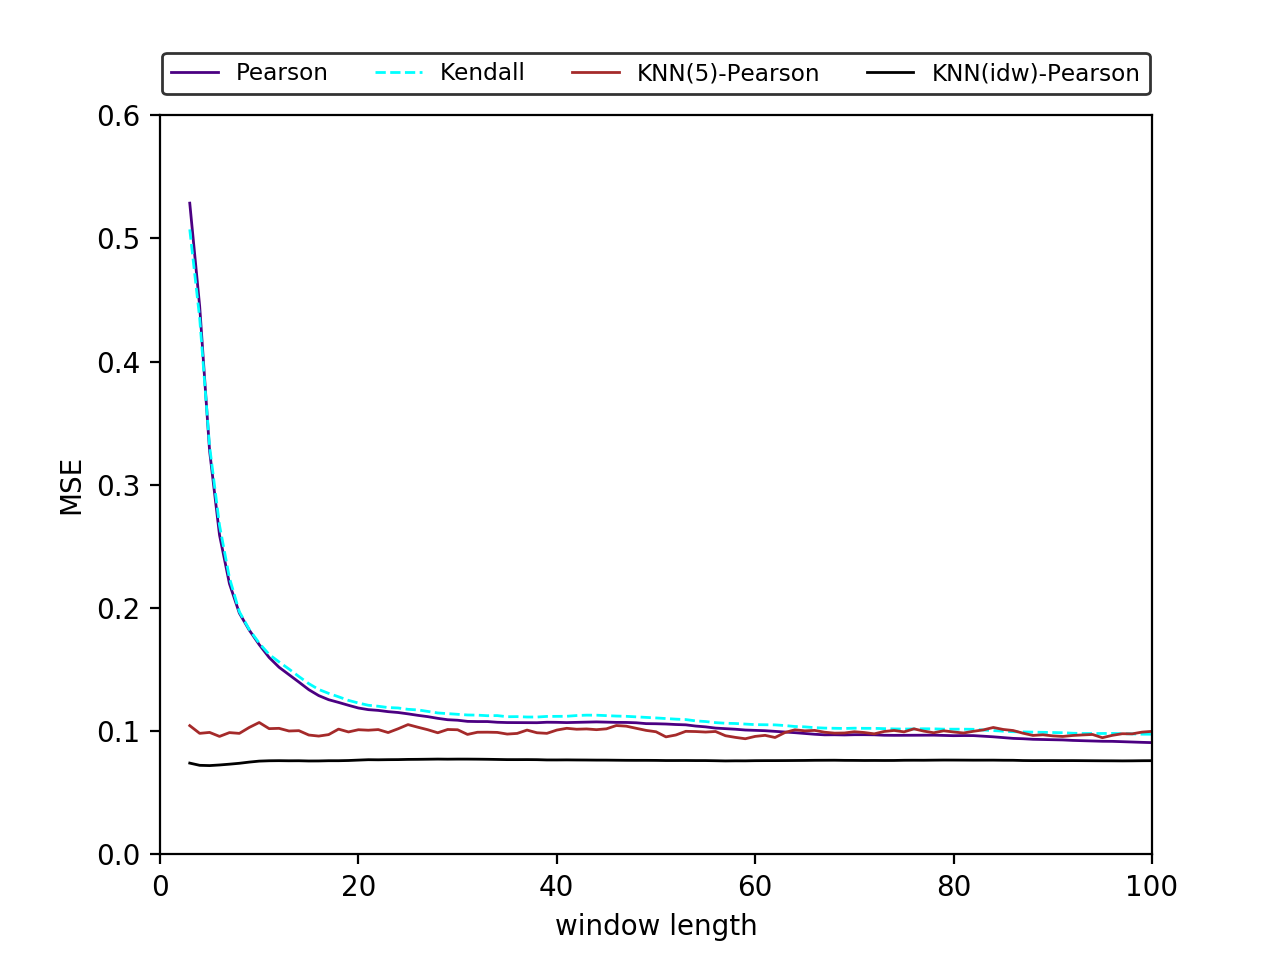
\includegraphics[width=\textwidth]{mse_knn5_idw_pearson_kendall_true} 
		\caption{MSE for KNN with Pearson covariates and true correlation, Pearson and Kendall Moving Window bootstrap estimates.}
		\label{fig:mse_knn5_idw_pearson_kendall_true}
	\end{subfigure}
	\hfill
	\begin{subfigure}[b]{0.49 \textwidth}
		\centering 
		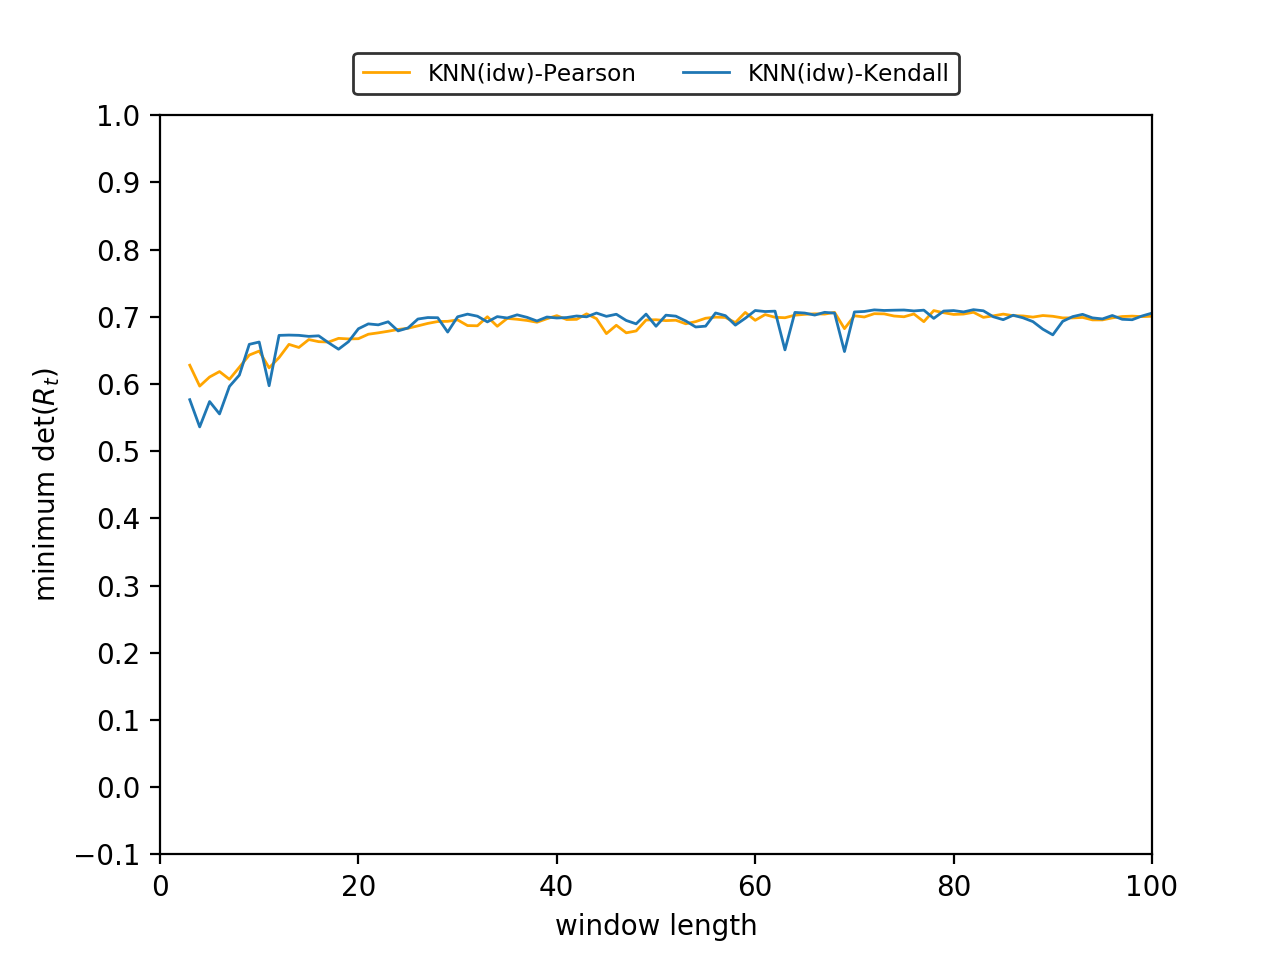
\includegraphics[width=\textwidth]{det_knn_IDW_pearson_kendall_true.png} 
		\caption{Minimum determinants for KNN estimates constructed from inverse distance weighting function, Pearson and Kendall covariates and true correlation.}
		\label{fig:det_knn_IDW_pearson_kendall_true.png}
	\end{subfigure}
	\caption{Comparison MSE and minimum determinants for KNN with true correlation, Pearson and Kendall Moving Window bootstrap estimates.}
	\label{fig:mse_det_knn5_idw_pearson_kendall_true}
\end{figure}


%%%%%%% RANDOM FOREST TRUE COR %%%%%%%%%%%%%%
\subsection{Random Forest}  \label{sec:rf_true_cor}
In order to obtain time-varying correlations, $\rho_t$, with random forests algorithm, the set of covariates is defined by lagged Pearson and Kendall moving window estimates and minimum and maximum asset return values from the last period, denoted by $min_{i}(r_{i,t-1})$, and $max_{i}(r_{i,t-1})$, respectively.  \\

\subsubsection{Diagnosing the Generalization Error of Random Forest}
The accuracy of RF estimates with Pearson and Kendall covariates for time-varying correlation is compared by using mean squared error (MSE) between estimated and actual correlations. MSE from RF with Pearson and Kendall moving window estimates of correlation for covariates are shown in Fig. \ref{fig:mse_rf10_pearson_kendall_true}. Regardless of the choice of window length, MSE from RF with Pearson and Kendall covariates are between 0.0847 and 0.0980, and 0.0830 and 0.0983, respectively. The variance of MSE from RF estimates with Pearson covariates is approximately 8.42e-6 while that of RF estimates with Kendall covariates is approximately 8.92e-6. Analogous to KNN estimates of correlation, RF thus appears to be rather insensitive to the choice of window length, regardless whether the set of covariates is constructed from Pearson or Kendall moving window estimates of correlation. \\

\noindent
Moreover, RF estimates of time-varying correlation where the set of covariates is constructed from Pearson and Kendall moving window estimates and true correlation as response variable satisfy the positive semi-definiteness condition in the time-varying correlation matrix $R_t$ for all time $t$ under all considered choices of window length. Fig. \ref{fig:det_rf10_pearson_kendall_true} presents the obtained minimum determinants of $R_t$ for all choices of window length.   

\begin{figure}[H]
	\centering
	\begin{subfigure}[b]{0.49 \textwidth} 
		\centering
		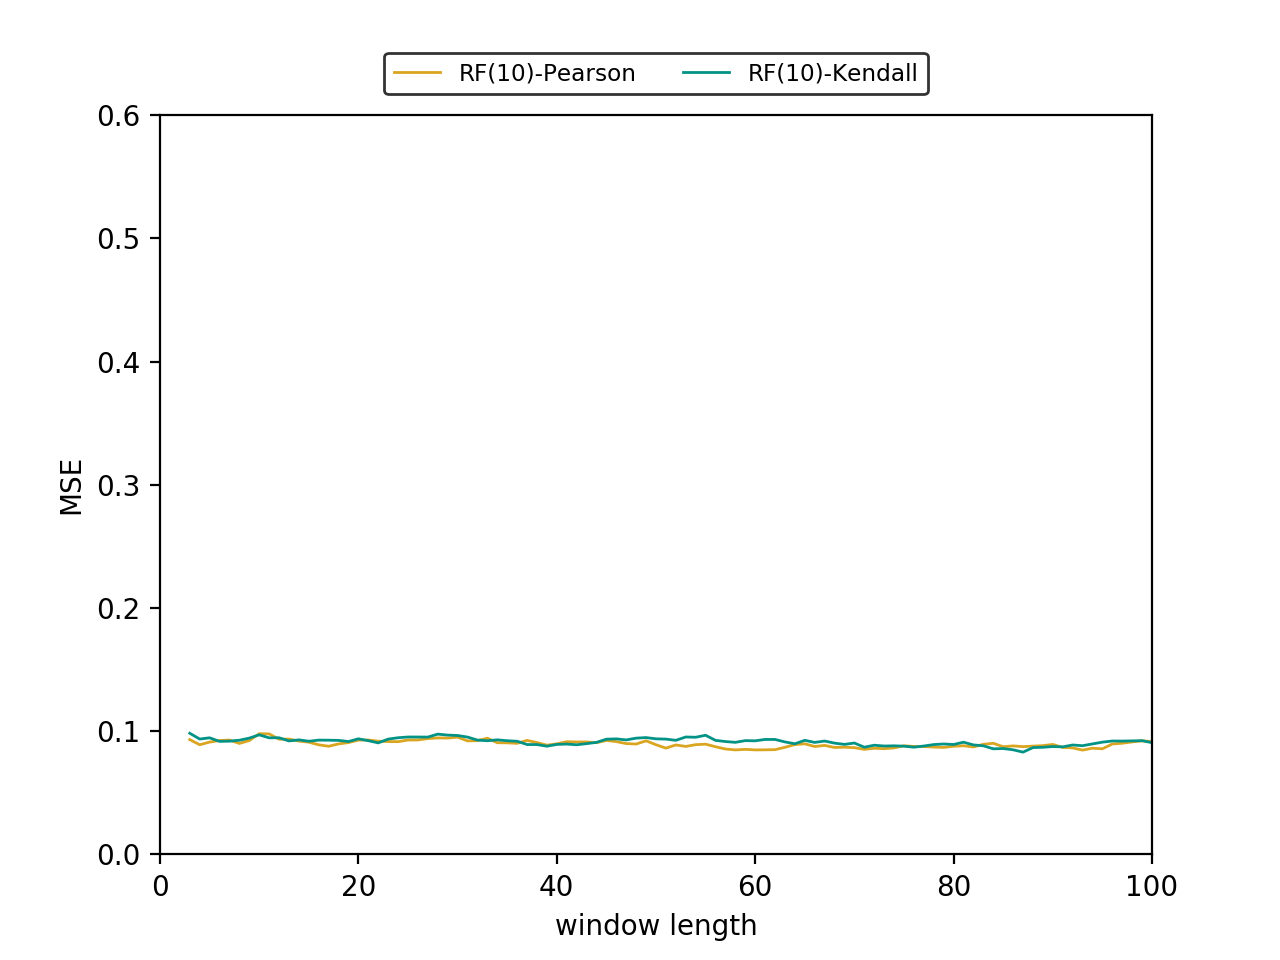
\includegraphics[width=\textwidth]{mse_rf10_pearson_kendall_true}
		\caption{MSE for RF with covariates from Pearson and Kendall and true correlation.}
		\label{fig:mse_rf10_pearson_kendall_true}
	\end{subfigure}
	\hfill
	\begin{subfigure}[b]{0.49 \textwidth} 
		\centering
		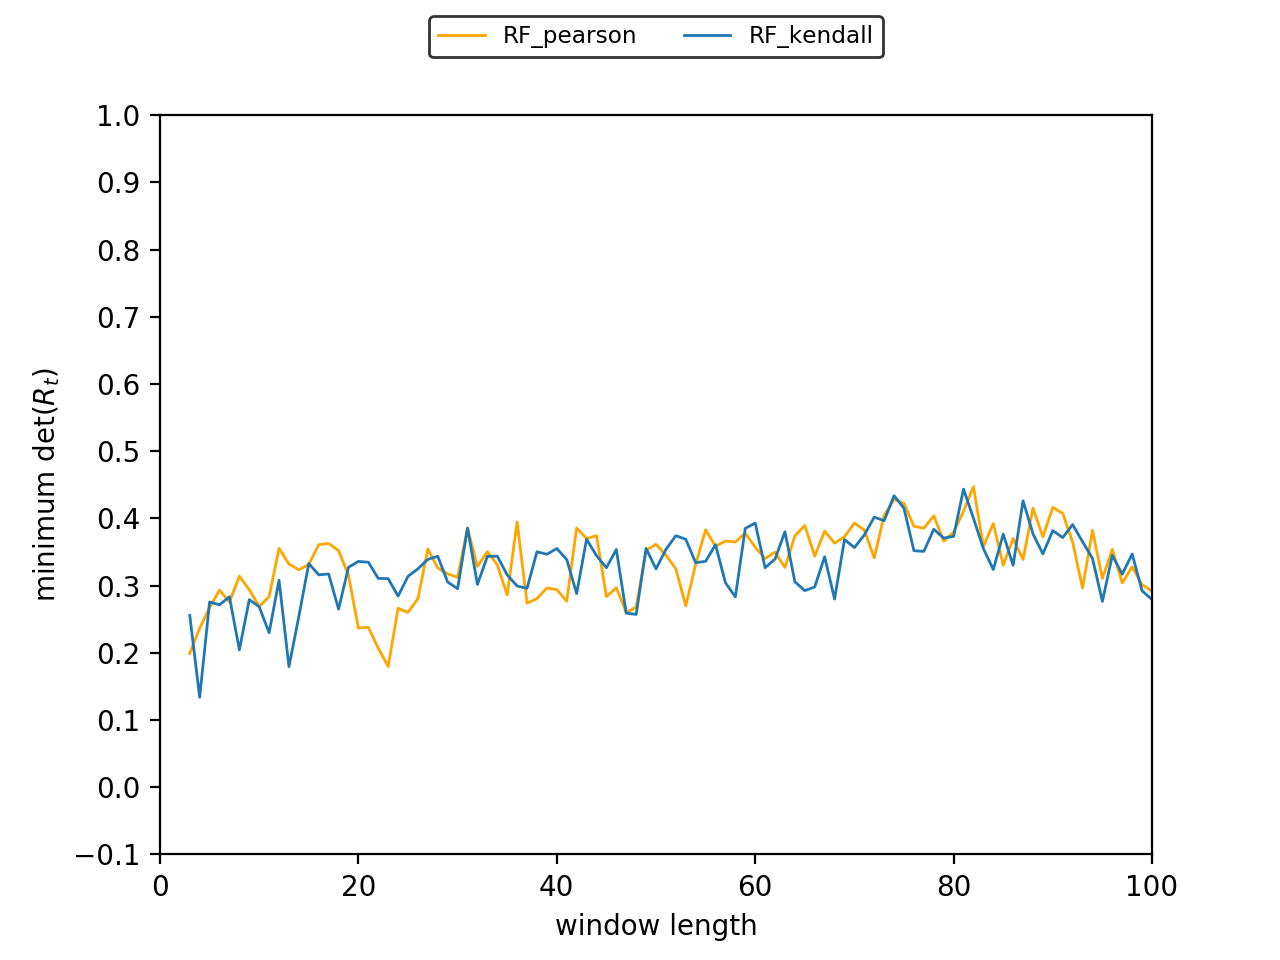
\includegraphics[width=\textwidth]{det_rf10_pearson_kendall_true}
		\caption{Minimum determinants for RF with covariates from Pearson and Kendall and true correlation.}
		\label{fig:det_rf10_pearson_kendall_true}
	\end{subfigure}
	\caption{Comparison MSE and minimum determinants for RF(n\_estimators=10) with covariates from Pearson and Kendall and true correlation.}
	\label{fig:mse_det_rf10_pearson_kendall_true}
\end{figure}

\noindent
From visual inspection of the plots in Fig. \ref{fig:rf_pearson21_bootstrap_true} and Fig. \ref{fig:rf_kendall21_bootstrap_true} it seems that the uncertainty in the time-varying correlation $\rho_t$, which is illustrated by the 99\% confidence interval, seems smaller for RF estimates compared to Pearson and Kendall moving window estimates under the same window length of 21. Analogous to KNN estimates of correlation, RF estimates of correlation with number of trees equal to 10 are much more volatile than Pearson and Kendall moving window estimates. This may be a less desirable result as it is not expected that correlation between assets changes that drastically at each time unit. Rather, correlation is expected to vary gradually over time \citep{ref:Basturk2016} \\

\noindent
The MSE decompositions into bias and variance terms from RF estimates of correlation are shown in Fig. \ref{fig:decom_mse_rf10_pearson_true} and Fig. \ref{fig:decom_mse_rf10_kendall_true}. These figures indicate that the RF algorithm is considerably less sensitive to the choice of the window length for smaller window sizes when compared to Pearson and Kendall moving window estimates of correlation depicted in Fig \ref{fig:mse_pearson_kendall_bootstrap}. The uncertainty around the estimated correlations appears to be marginally affected by the choice of the window length for all window sizes. This statement is supported by the fact that the variance as a function of the window length behaves like a (more or less) constant red line in these figures; a result analogous to KNN estimates of correlation.


\begin{figure}[H]  % [h] parameter makes sure figures are located at 'this' location.
	\centering
	\begin{subfigure}[b]{0.49 \textwidth} % sum of widths should be less than text width if all one the same line
		\centering 
		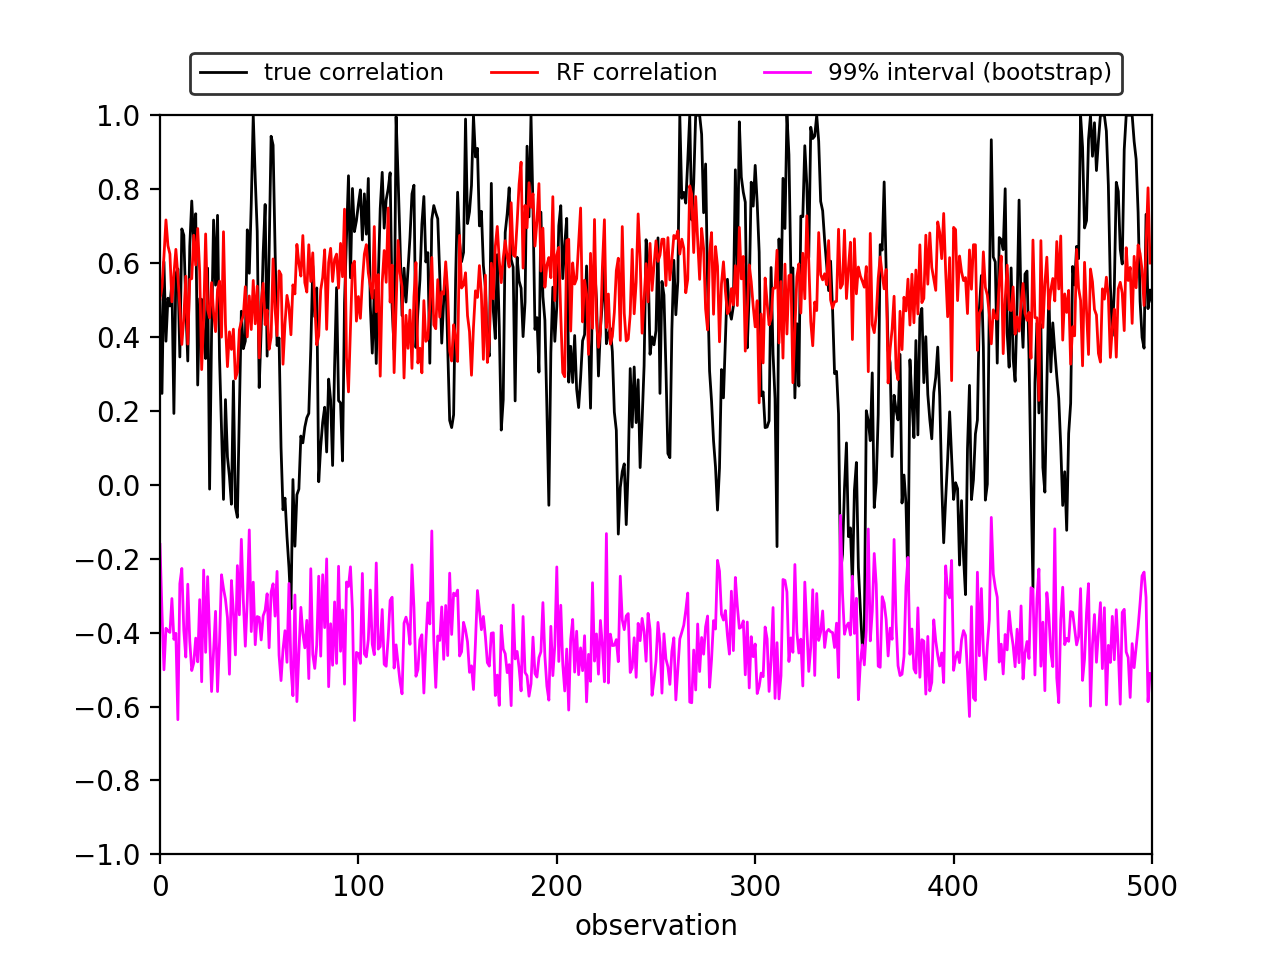
\includegraphics[width=\textwidth]{rf_pearson_21_estimates_bootstrap_true.png} 
		\caption{RF estimates with window size 21, Pearson as covariate and true correlation.} 	
		\label{fig:rf_pearson21_bootstrap_true}
	\end{subfigure} 
	\hfill	
	\begin{subfigure}[b]{0.49 \textwidth} 
		\centering 
		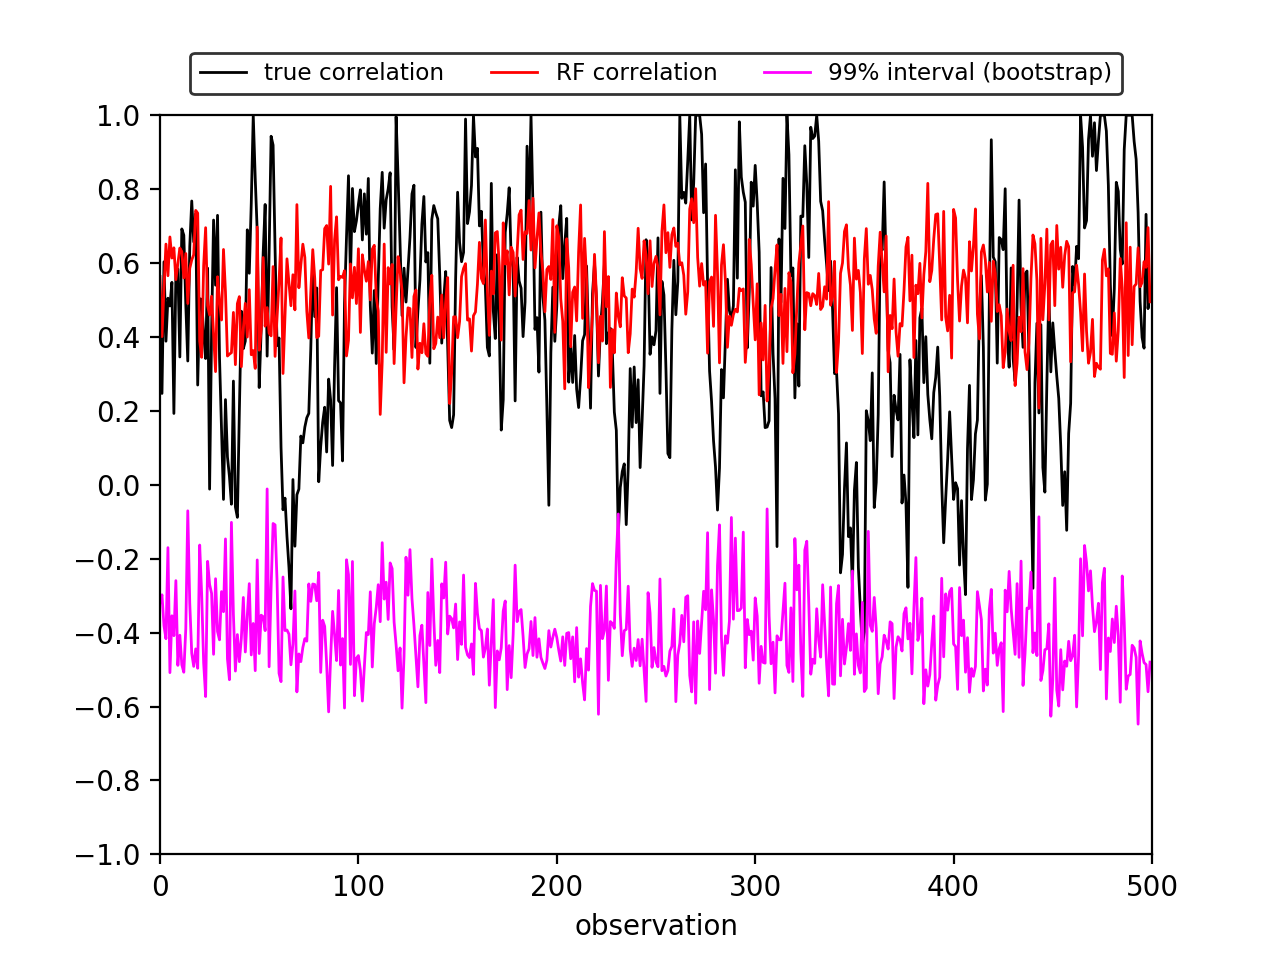
\includegraphics[width=\textwidth]{rf_kendall_21_estimates_bootstrap_true.png} 
		\caption{RF estimates with window size 21, Kendall as covariate and true correlation.} 
		\label{fig:rf_kendall21_bootstrap_true}
	\end{subfigure} 
	\hfill	
	\begin{subfigure}[b]{0.49 \textwidth}
		\centering 		
		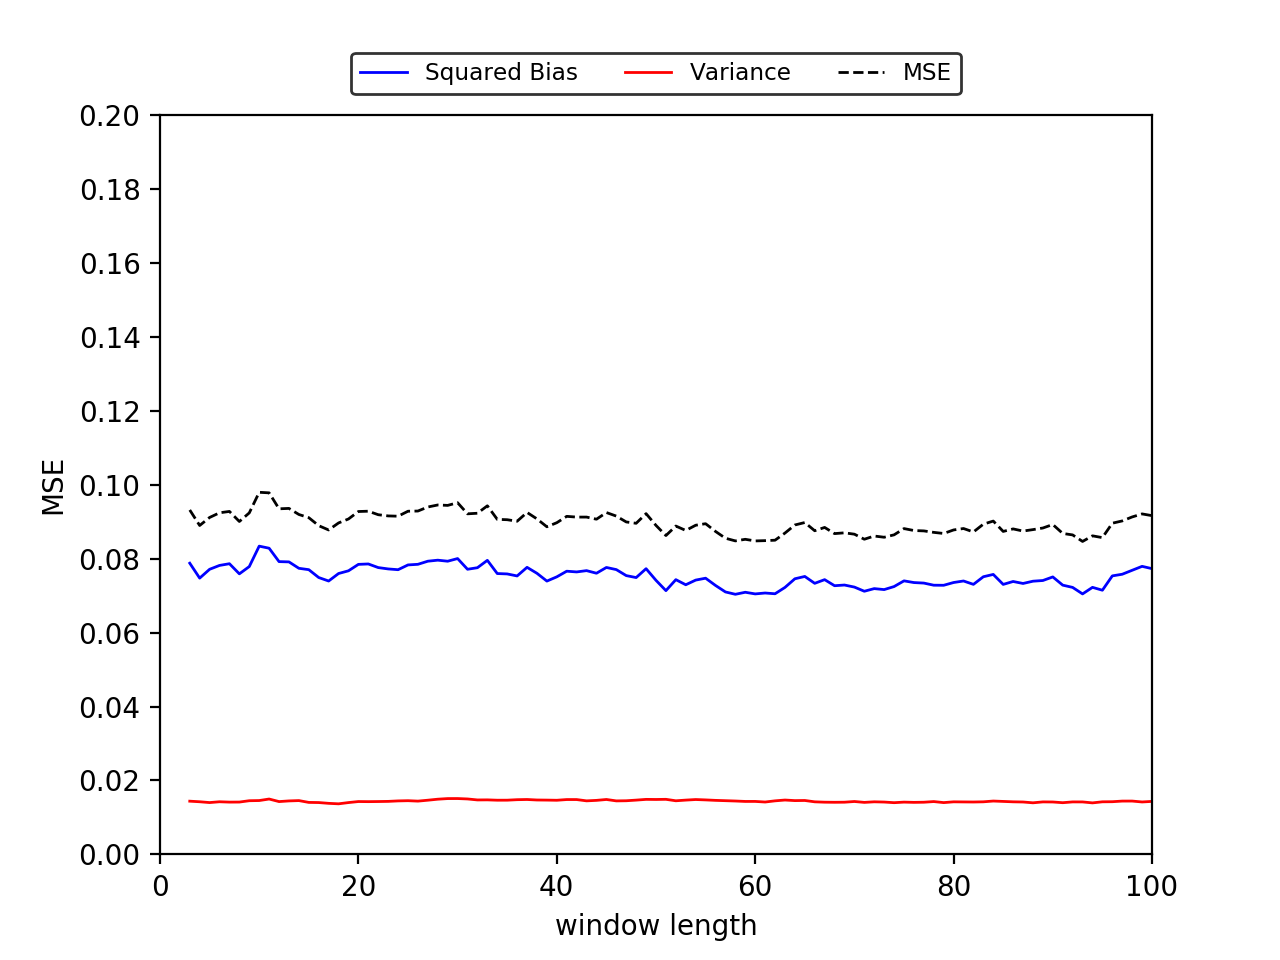
\includegraphics[width=\textwidth]{decom_mse_rf10_pearson_true.png} 
		\caption{Bias-variance decomposition for RF estimates with Pearson as covariate and true correlation.} 
		\label{fig:decom_mse_rf10_pearson_true}
	\end{subfigure}
	\hfill  
	\begin{subfigure}[b]{0.49 \textwidth}
		\centering 
		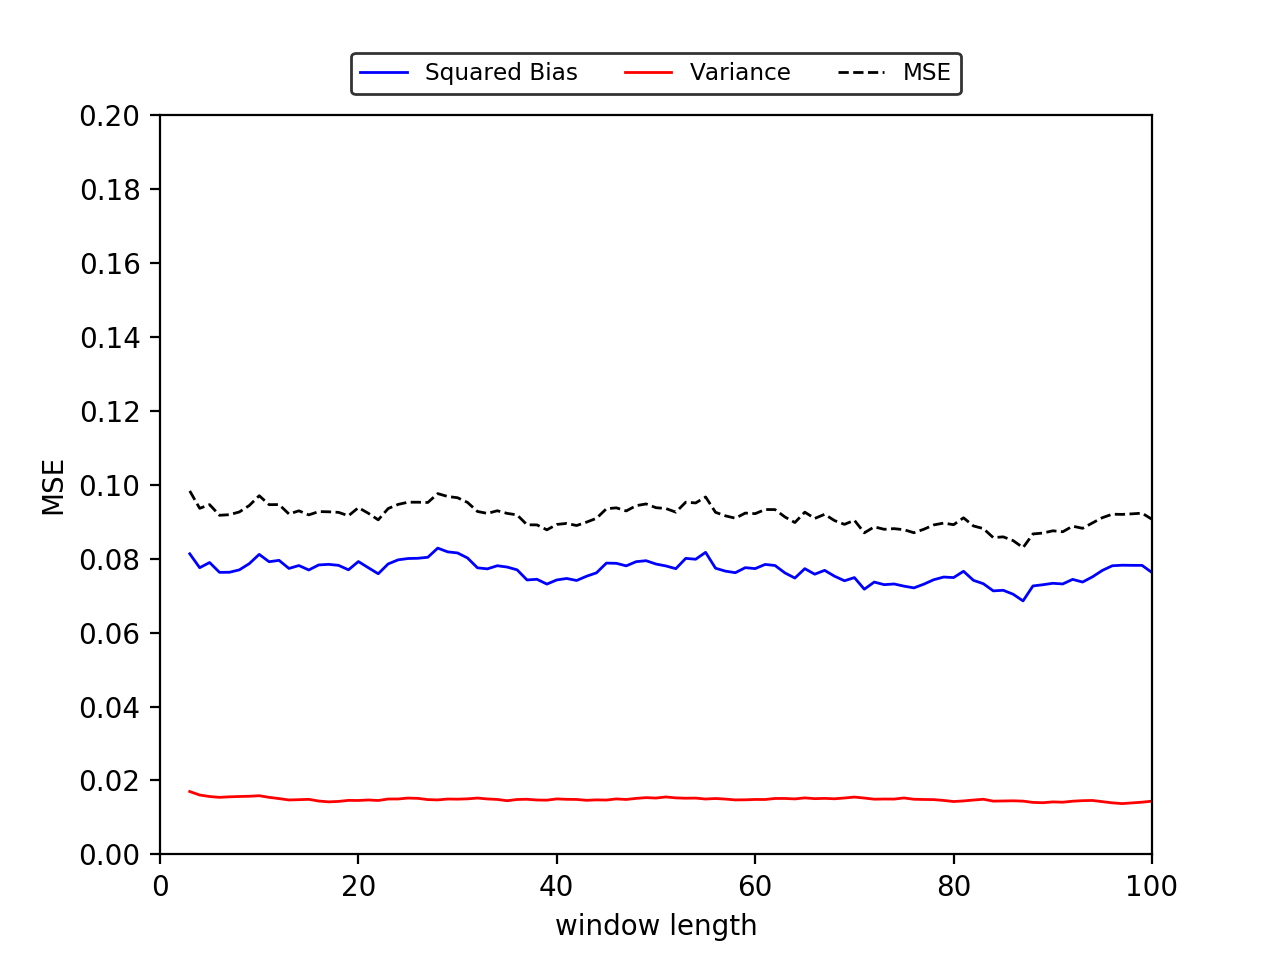
\includegraphics[width=\textwidth]{decom_mse_rf10_kendall_true.png} 
		\caption{Bias-variance decomposition for RF estimates with Kendall as covariate and true correlation.} 
		\label{fig:decom_mse_rf10_kendall_true}
	\end{subfigure}
	\caption{MSE for RF estimates with Pearson and Kendall Moving Window bootstrap estimates as covariates and true correlation.}
	\label{fig:decom_mse_rf10_pearson_kendall_true}
\end{figure}

\subsubsection{Alternative Parameterizations of Random Forest Algorithm}
\textbf{State that we take 100 bootstrapped samples instead of 1000 due to computational constraints. This number of bootstrapped samples will however be sufficient for illustrational purposes.} \\

\noindent
Simulation results in Tabel \ref{tab:mse_decomp_rf_pearson_kendall_true} show an inverse relationship between the choice of the number of estimators (trees) in the random forest used in the estimation of correlations and the uncertainty around the estimated correlations, regardless whether Pearson or Kendall estimates are used for defining the set of covariates. It is clearly observed that an increase in the number of estimators results in a decrease of the variance, and conversely. This observation is in line with our discussion on MSE decomposition for the RF algorithm and Eq. \eqref{eq:variance_rf} from Section \ref{sec:mse_decompose}. For this particular dataset it is observed that the point of diminishing reduction in variance is reached around 300 trees. An increase in number of trees after that does not significantly reduces the variance. \\  




%% TABLE
\begin{table}[H]
\centering
\captionsetup[subtable]{position=below}
%\captionsetup[table]{position=below}
\begin{subtable}{0.49\linewidth}
\centering
\begin{tabular}{r  c  c  c} 
\toprule
\multicolumn{1}{ r }{\textbf{Trees}} &
\multicolumn{1}{ c }{\textbf{Squared Bias}} &
\multicolumn{1}{ c }{\textbf{Variance}} &
\multicolumn{1}{ c }{\textbf{MSE}} \\
\midrule 

10                                   &   0.0839                       & 0.0144                & 0.0983      \\
100                                 & 0.0839                         & 0.0077               & 0.0916       \\
300                                 & 0.0837                         & 0.0071               & 0.0908      \\
600                                 & 0.0841                         & 0.0070               & 0.0911     \\
1000                               & 0.0837                         &  0.0069              & 0.0906     \\ [1ex]

\bottomrule
\end{tabular}
\caption{MSE for RF estimates with window size 10, Pearson as covariate and true correlation.}
\label{tab:mse_decomp_rf_pearson_true}
\end{subtable}
\hfill
\begin{subtable}{0.49\linewidth}
\centering
\begin{tabular}{r  c  c  c} 
\toprule
\multicolumn{1}{ r }{\textbf{Trees}} &
\multicolumn{1}{ c }{\textbf{Squared Bias}} &
\multicolumn{1}{ c }{\textbf{Variance}} &
\multicolumn{1}{ c }{\textbf{MSE}} \\
\midrule 

10                                   & 0.0817                         & 0.0158               &  0.0976     \\
100                                 & 0.0815                         & 0.0088               & 0.0903      \\
300                                 & 0.0813                         & 0.0082               & 0.0895      \\
600                                 & 0.0817                         & 0.0082               & 0.090     \\
1000                               &  0.0814                         &  0.0080             & 0.0894     \\ [1ex]

\bottomrule
\end{tabular}
\caption{MSE for RF estimates with window size 10, Kendall as covariate and true correlation.}
\label{tab:mse_decomp_rf_kendall_true}
\end{subtable}
\caption{Mean Squared Error (MSE) decomposition as a function of the number of estimators (trees) for RF with proxy for covariates and true correlation.}
\label{tab:mse_decomp_rf_pearson_kendall_true}
\end{table}

\noindent
\textbf{Insert sensitivity  analysis where MSE is a function of number of covariates used in the tree construction process of random forest algorithm.}  \\


\noindent
This section is concluded with a comparison of the function approximation capabilities of the RF algorithm and Pearson and Kendall moving window estimates. The comparison is based on MSE between estimated and actual correlations. Fig. \ref{fig:mse_rf10_pearson_kendall_comp_true.png} shows MSE from RF with default parameterization, i.e. number of estimators equals 10, as well as Pearson and Kendall moving window estimates of time-varying correlations. According to MSE, default parameterizations of the RF algorithm where the random forest is constructed from 10 estimators (trees) results in significantly smaller MSE compared to Pearson and Kendall moving window estimates for all window sizes. Finally, the variance of MSE from RF estimates with default parameterization and Pearson and Kendall approximations of true correlation in Fig. \ref{fig:mse_rf10_pearson_kendall_comp_true.png} are 8.42e-6 and 8.92e-6, respectively, while that of Pearson and Kendall moving window estimates are 0.0040 and 0.0037, respectively. \\


\begin{figure}[H]
	\centering
	\begin{subfigure}[b]{0.49 \textwidth} 
		\centering
		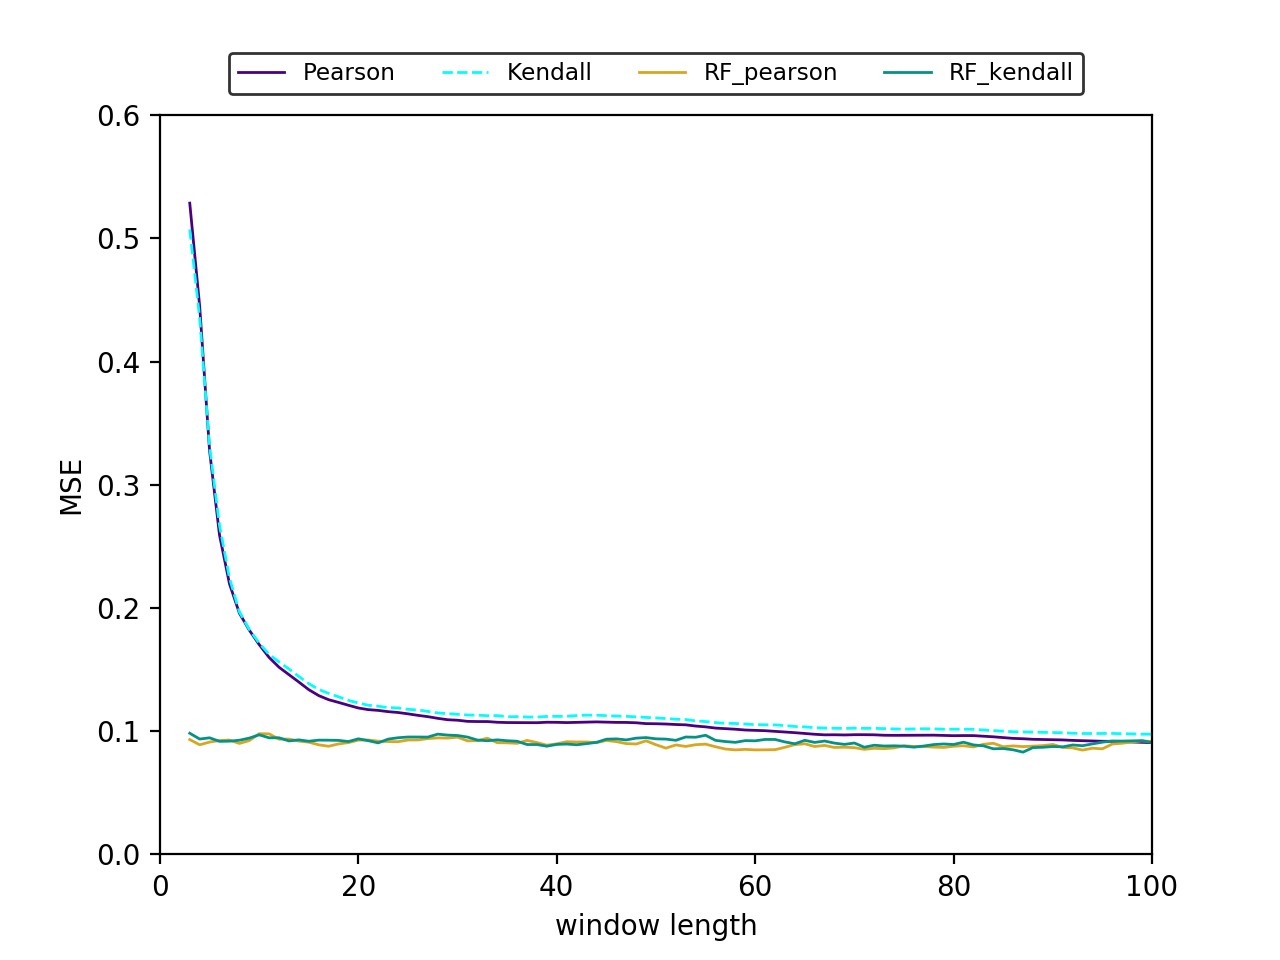
\includegraphics[width=\textwidth]{mse_rf10_pearson_kendall_comp_true.png}
		%\caption{MSE for RF with covariates from Pearson and Kendall and true correlation.}
		%\label{fig:mse_rf10_pearson_kendall_comp_true.png}
	\end{subfigure}
	\caption{Comparison MSE for RF(n\_estimators=10) with true correlation, Pearson and Kendall Moving Window bootstrap estimates.}
	\label{fig:mse_rf10_pearson_kendall_comp_true.png}
\end{figure}

\noindent
\textbf{Perhaps add RF(n\_estimators=100) to show that this parameterization performs even better due to variance reduction. Maybe mentioning this with reference to the sensitivity analysis is also sufficient.} 






%%%%%%%%%%%%%%%%%%%%%%%%%%%%%%%%%%%%%
%%%%%%%%%% Proxies for Correlation %%%%%%%%%%%%%%%%
%%%%%%%%%%%%%%%%%%%%%%%%%%%%%%%%%%%%%%
\section{Learning with Proxies for Response Variable and Covariates} \label{sec:proxy_correlation}
In this section, a more realistic approach is taken to the application of nearest neighbors and random forests algorithms for time-varying correlation estimation. Both the covariates and response variable are obtained from moving window estimation, as defined in \eqref{eq:mw_rho} and \eqref{eq:mw_kendall}. This is different from Sec. \ref{sec:true_correlation} where the response variable of the learning algorithms was defined as the true observed correlation (given by the simulated parameters). \textbf{Relate this section to the research question how learning algorithms perform/ behave when the response variable contains noise in the form of approximation error.} \\

\noindent
\textit{A fourth issue is the degree of noise in the desired output values (the supervisory target variables). If the desired output values are often incorrect (because of human error or sensor errors), then the learning algorithm should not attempt to find a function that exactly matches the training examples. Attempting to fit the data too carefully leads to overfitting. You can overfit even when there are no measurement errors (stochastic noise) if the function you are trying to learn is too complex for your learning algorithm. In such a situation, the part of the target function that cannot be modeled "corrupts" your training data - this phenomenon has been called deterministic noise. When either type of noise is present, it is better to go with a higher bias, lower variance estimator.}

%%%%%% NEAREST NEIGHBOR PROXY 	%%%%%%%%
\subsection{Nearest Neighbor} \label{sec:knn_proxy_cor}
In this section, results from application of the KNN algorithm will be compared to those obtained by Pearson and Kendall moving window estimation, as depicted in Fig. \ref{fig:decom_mse_pearson_kendall_true}. The uncertainty in the time varying-correlation $\rho_t$, which is illustrated by the 99\% confidence interval, is much smaller compared to MW, even though both the set of covariates and the response variable of the KNN algorithm are based on approximations of correlation instead of actual correlation. \\

\subsubsection{Diagnosing the Generalization Error of Nearest Neighbor}
The accuracy of KNN estimates with Pearson and Kendall moving window estimates for both covariates and response variable is compared by using mean squared error (MSE) between estimated and actual correlations. MSE from KNN with Pearson and Kendall moving window estimates of correlation is shown in Fig. \ref{fig:mse_knn5_pearson_kendall_proxy}. Regardless of the choice of window length, MSE from KNN with Pearson and Kendall covariates are between 0.0855 and 0.2555, and 0.0952 and 0.2223, respectively. The variance of MSE from KNN estimates with Pearson covariates is approximately 5.70e-4 while that of KNN estimates with Kendall covariates is approximately 2.96e-4. Recall that in Fig. \ref{fig:mse_knn5_pearson_kendall_true} KNN appeared to be insensitive to the choice of window length when true correlation is defined as the response variable. Interestingly, Fig. \ref{fig:mse_knn5_pearson_kendall_proxy} shows that MSE from KNN estimation with Pearson or Kendall approximations for the response variable varies substantially for smaller window sizes. Although, less variation is observed when compared with MSE from Pearson and Kendall moving window estimates depicted in Fig. \ref{fig:mse_pearson_kendall_bootstrap}. A possible explanation for this behaviour will be given towards the end of this section when comparing MSE between KNN estimates and Pearson and Kendall moving window estimates in more detail. \\

\noindent
Moreover, KNN estimates of time-varying correlation where the set of covariates is constructed from Pearson and Kendall moving window estimates and proxy correlation, satisfy the positive semi-definiteness condition in the time-varying correlation matrix $R_t$ for all time $t$ under all choices of window length. Fig. \ref{fig:det_knn5_pearson_kendall_proxy} presents the obtained minimum determinants of $R_t$ for all choices of window length.  
     
\begin{figure}[H]
	\centering
	\begin{subfigure}[b]{0.49 \textwidth} 
		\centering
		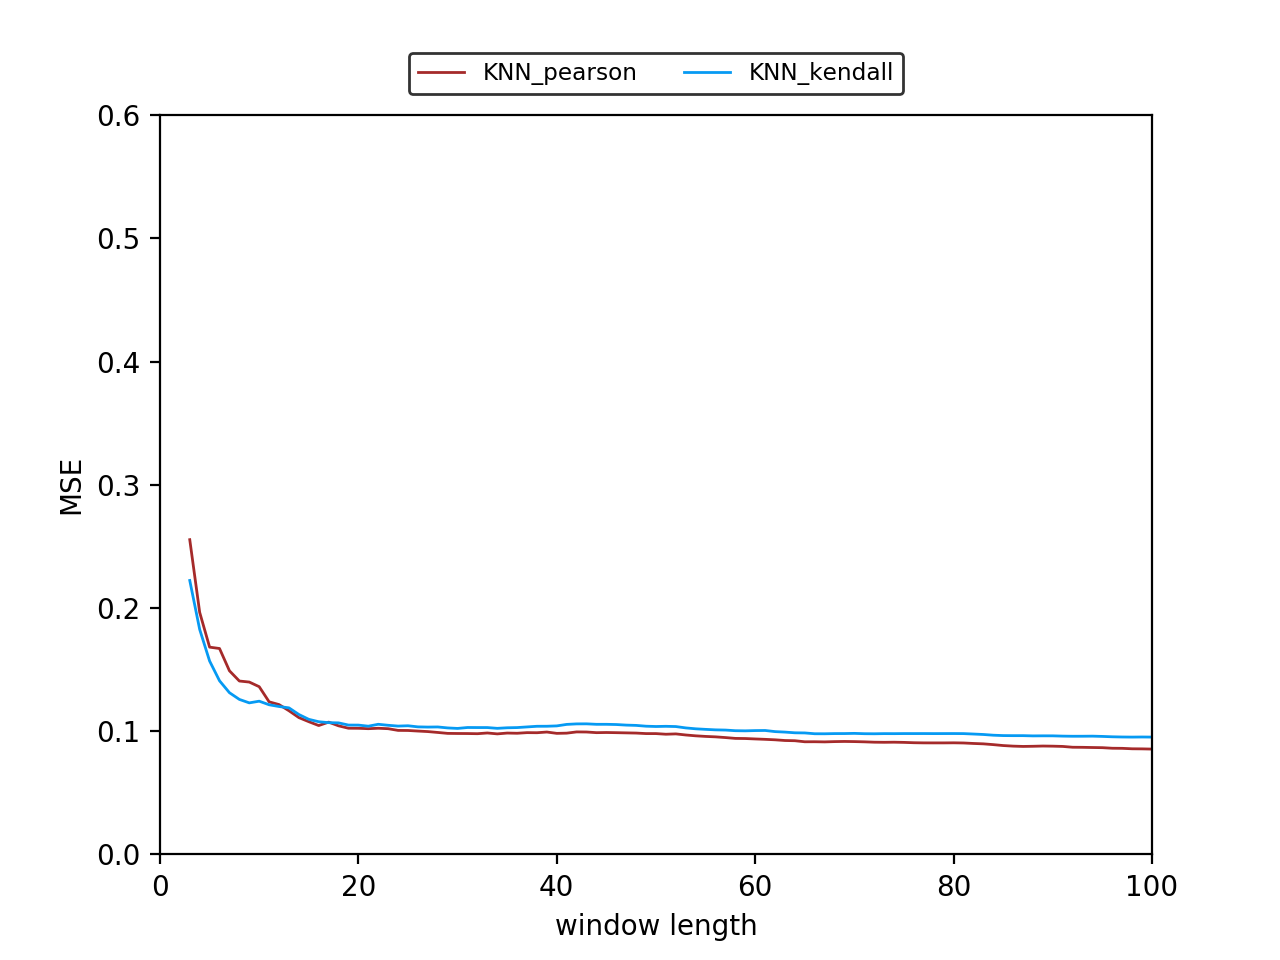
\includegraphics[width=\textwidth]{mse_knn5_pearson_kendall_proxy.png}
		\caption{MSE for KNN with covariates from Pearson and Kendall and proxy correlation.}
		\label{fig:mse_knn5_pearson_kendall_proxy}
	\end{subfigure}
	\hfill
	\begin{subfigure}[b]{0.49 \textwidth} 
		\centering
		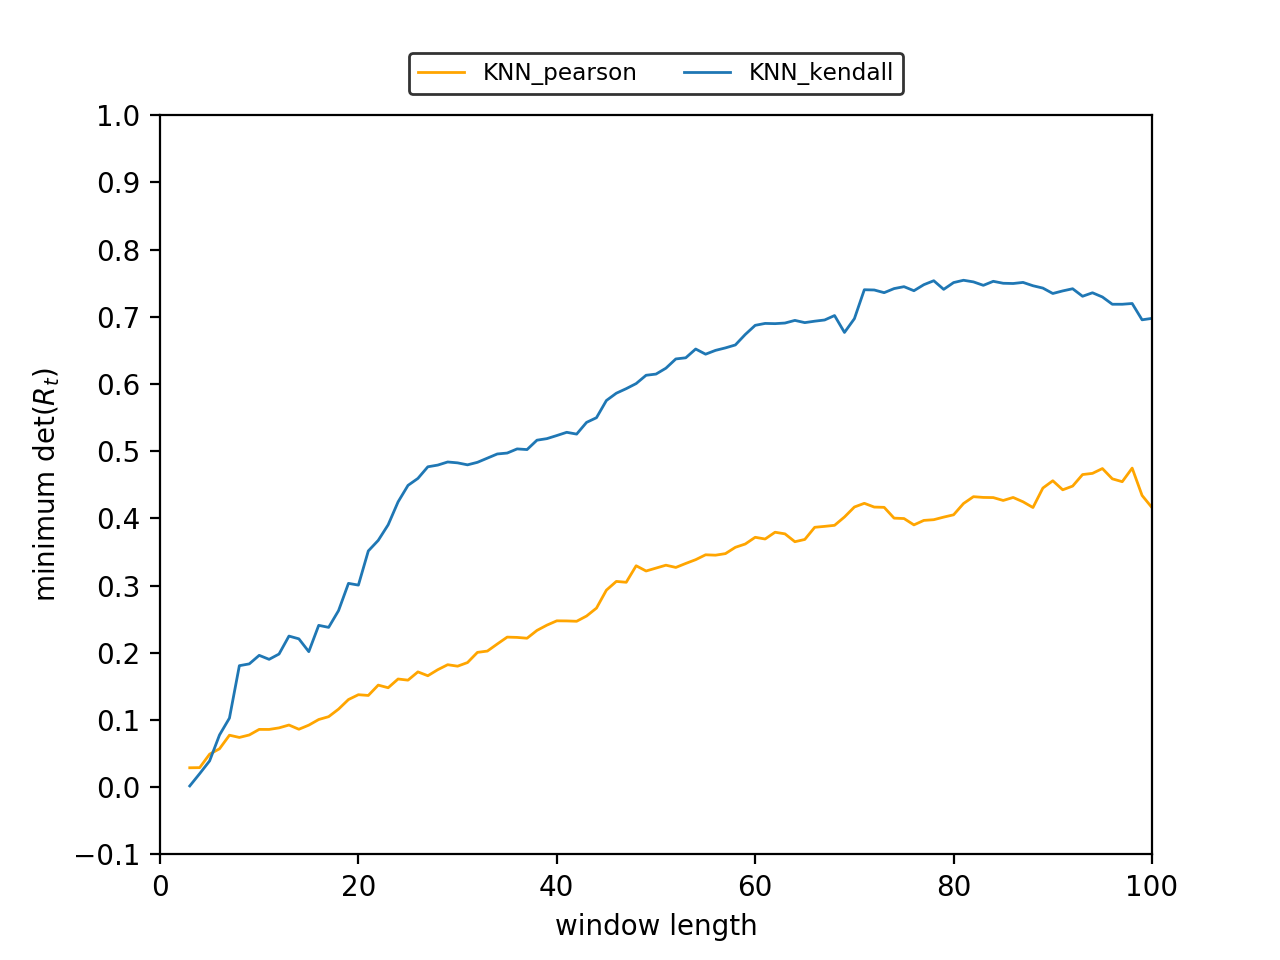
\includegraphics[width=\textwidth]{det_knn5_pearson_kendall_proxy}
		\caption{Minimum determinants for KNN with covariates from Pearson and Kendall and proxy correlation.}
		\label{fig:det_knn5_pearson_kendall_proxy}
	\end{subfigure}	
	\caption{Comparison MSE and minimum determinants for KNN(n\_neighbors=5) with covariates from Pearson and Kendall and proxy correlation.}
	\label{fig:mse_det_knn5_pearson_kendall_proxy}
\end{figure}

\noindent
From visual inspection of the plots in Fig. \ref{fig:knn_pearson21_bootstrap_proxy} and Fig. \ref{fig:knn_kendall21_bootstrap_proxy} it is clear that the uncertainty in the time-varying correlation $\rho_t$, 
which is illustrated by the $99\%$ confidence interval, is smaller for KNN estimates compared to Pearson moving window estimates and Kendall moving window estimates, even though both the set of covariates and the response variable of the KNN algorithm are based on approximations of correlation instead of actual correlation. These figures also show smaller uncertainty in the time-varying correlation $\rho_t$ when compared with KNN estimates with true correlation as the response variable, which are depicted in Fig. \ref{fig:decom_mse_knn5_pearson_kendall_proxy}. KNN estimates of correlation with true correlation as response variable in Fig. \ref{fig:knn_pearson21_bootstrap_proxy} and Fig. \ref{fig:knn_kendall21_bootstrap_proxy} are much more volatilte. KNN estimates with approximated correlation as response variable in Fig. \ref{fig:knn_pearson21_bootstrap_proxy} and Fig. \ref{fig:knn_kendall21_bootstrap_proxy}, however, follow the increases and decreases of the actual correlation smoother, with tighter confidence intervals. This is a more desirable result as it is not expected that correlation between assets changes that drastically at each time unit. \\


\noindent
The MSE decompositions into bias and variance terms from KNN estimates of correlation are shown in Fig. \ref{fig:decom_mse_knn_pearson_proxy} and Fig. \ref{fig:decom_mse_knn_kendall_proxy}. These figures indicate that the KNN algorithm with approximated output is more sensitive to the choice of the window length for smaller window sizes compared to KNN algorithm with true correlation depicted in Fig. \ref{fig:decom_mse_knn5_pearson_kendall_true}. This observation can be explained by error propagation: the effect of covariates' uncertainties (or errors) on the error of the function based on them. In the case when KNN algorithm uses proxies for response variables, the error associated with approximation of true correlation using moving window estimates is propagated to the output of the KNN algorithm. Fig. \ref{fig:decom_mse_knn_pearson_proxy} and Fig. \ref{fig:decom_mse_knn_kendall_proxy} show, however, that the KNN algorithm with approximated output is considerably less sensitive to the choice of the window length for smaller window sizes when compared to Pearson and Kendall moving window estimates of correlation depicted in Fig. \ref{fig:decom_mse_pearson} and Fig \ref{fig:decom_mse_kendall}, respectively. The KNN algorithm thus seems to mitigate the error propagation to some extend for smaller window sizes. This may be due to the fact that KNN, even with a small number of neighbors such as the default value of 5, estimates time-varying correlation using neighbors that contain additional informational value compared to the informational value in moving window estimates with small window sizes.      


\begin{figure}[H]  % [h] parameter makes sure figures are located at 'this' location.
	\centering
	\begin{subfigure}[b]{0.49 \textwidth} % sum of widths should be less than text width if all one the same line
		\centering 
		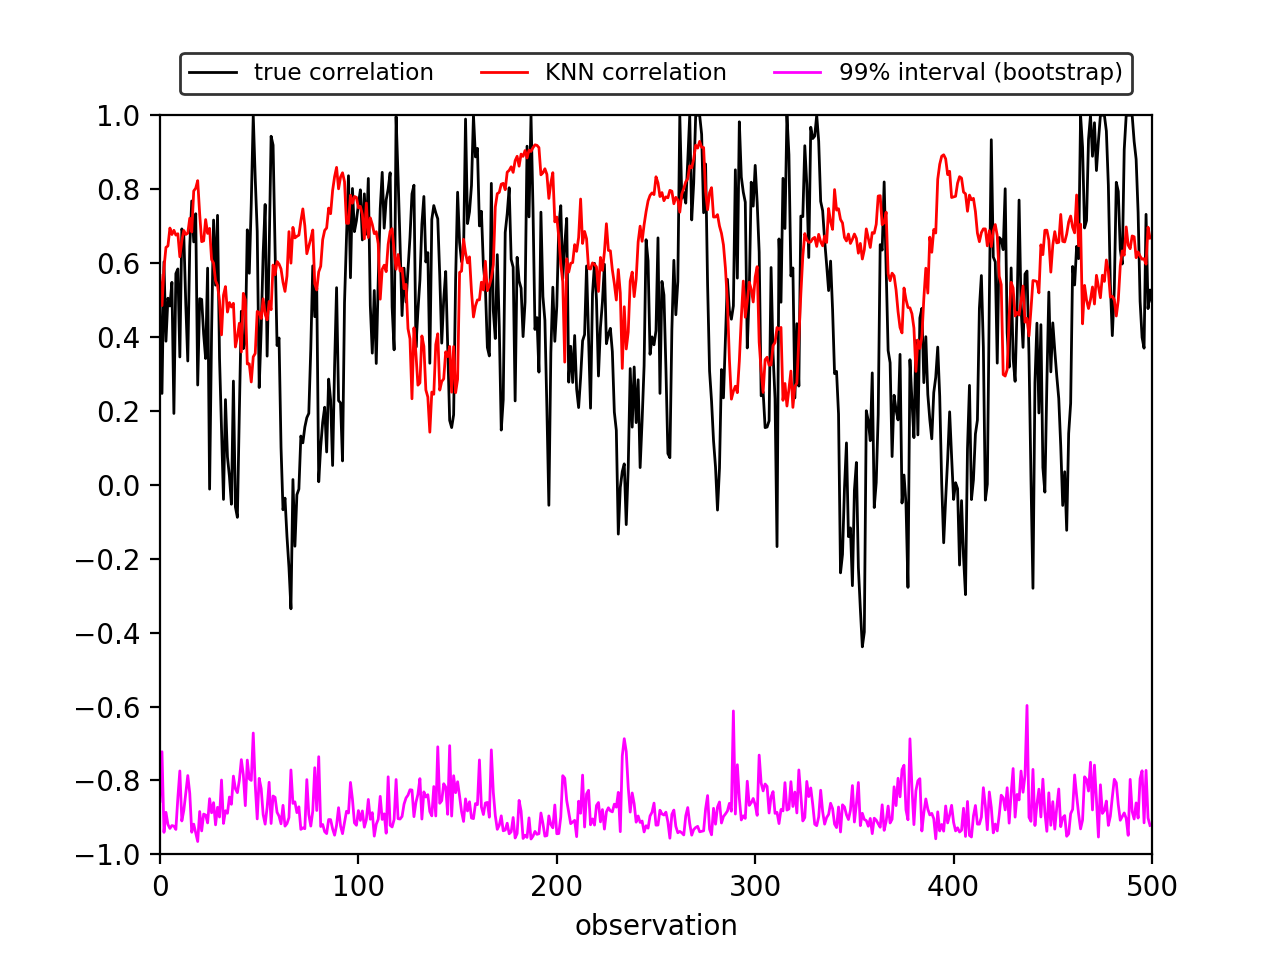
\includegraphics[width=\textwidth]{knn_pearson_21_estimates_bootstrap_proxy.png} 
		\caption{KNN estimates with window size 21, Pearson as covariate and proxy correlation.} 	
		\label{fig:knn_pearson21_bootstrap_proxy}
	\end{subfigure} 
	\hfill	
	\begin{subfigure}[b]{0.49 \textwidth} 
		\centering 
		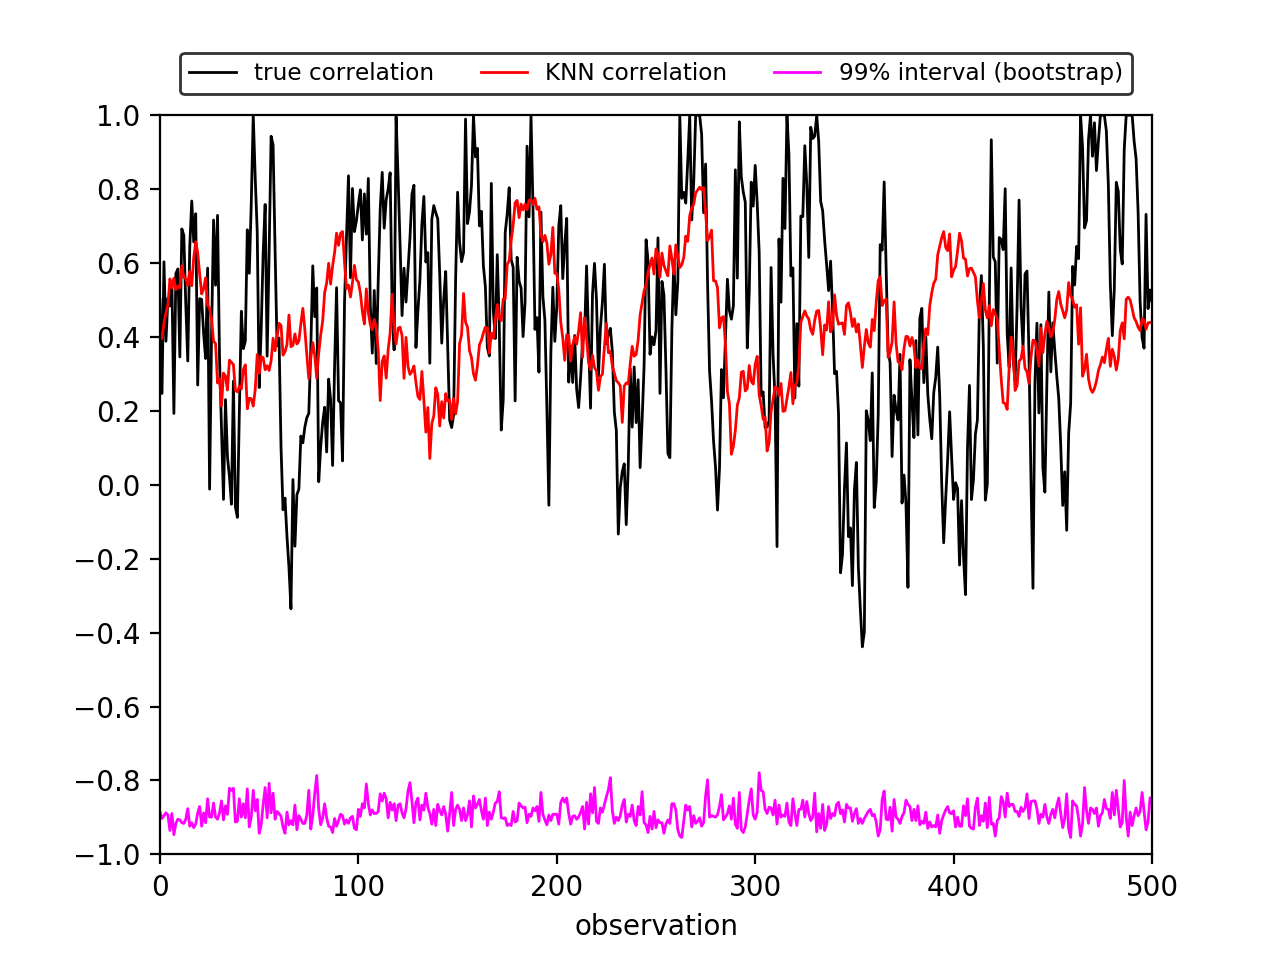
\includegraphics[width=\textwidth]{knn_kendall_21_estimates_bootstrap_proxy.png} 
		\caption{KNN estimates with window size 21, Kendall as covariate and proxy correlation.} 
		\label{fig:knn_kendall21_bootstrap_proxy}
	\end{subfigure} 
	\hfill	
	\begin{subfigure}[b]{0.49 \textwidth}
		\centering 
		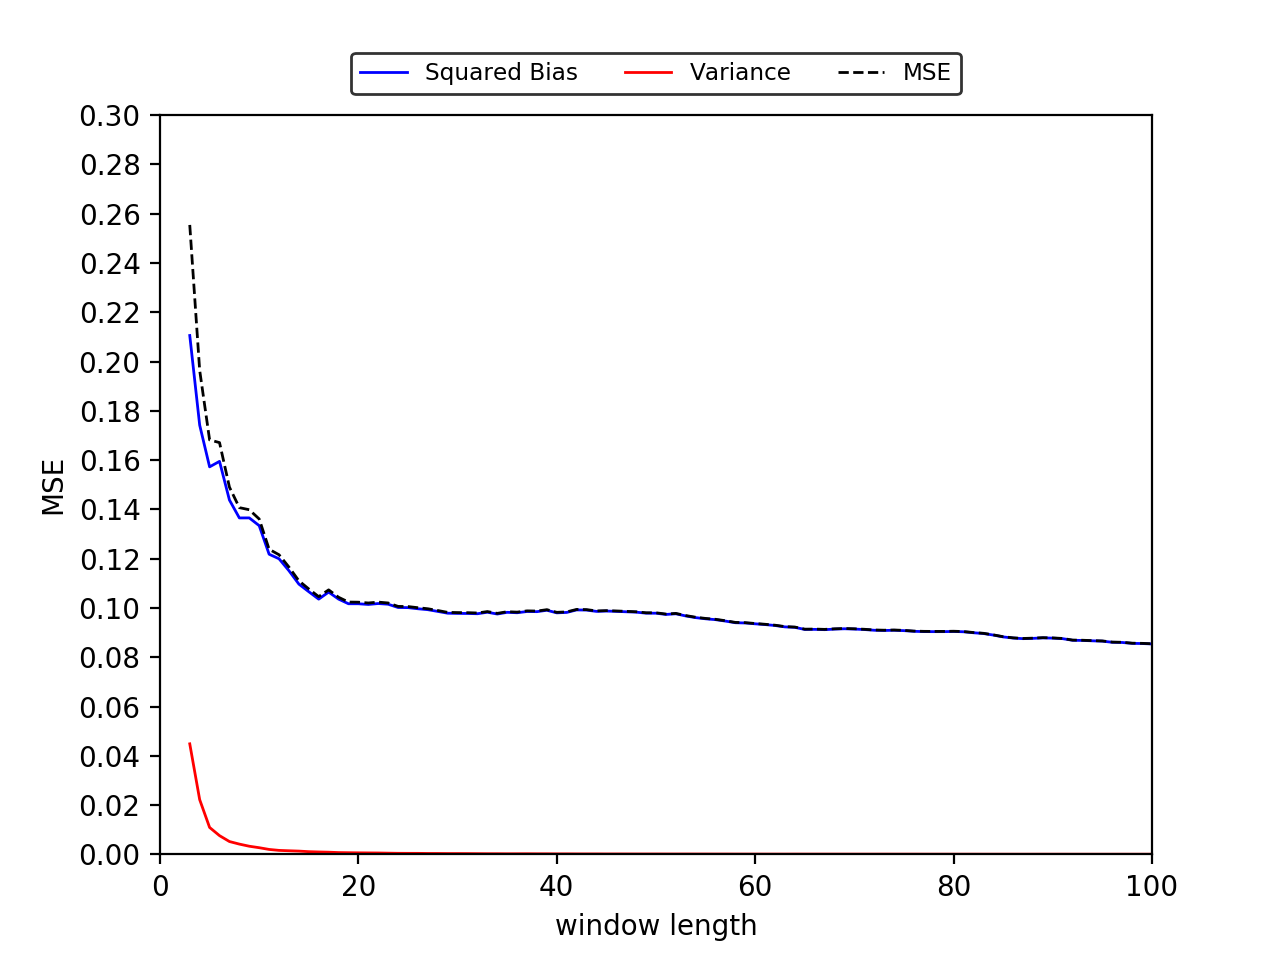
\includegraphics[width=\textwidth]{decom_mse_knn_pearson_proxy.png} 
		\caption{Bias-variance decomposition for KNN estimates with Pearson as covariate and proxy correlation.} 	
		\label{fig:decom_mse_knn_pearson_proxy}
	\end{subfigure}
	\hfill  
	\begin{subfigure}[b]{0.49 \textwidth}
		\centering 
		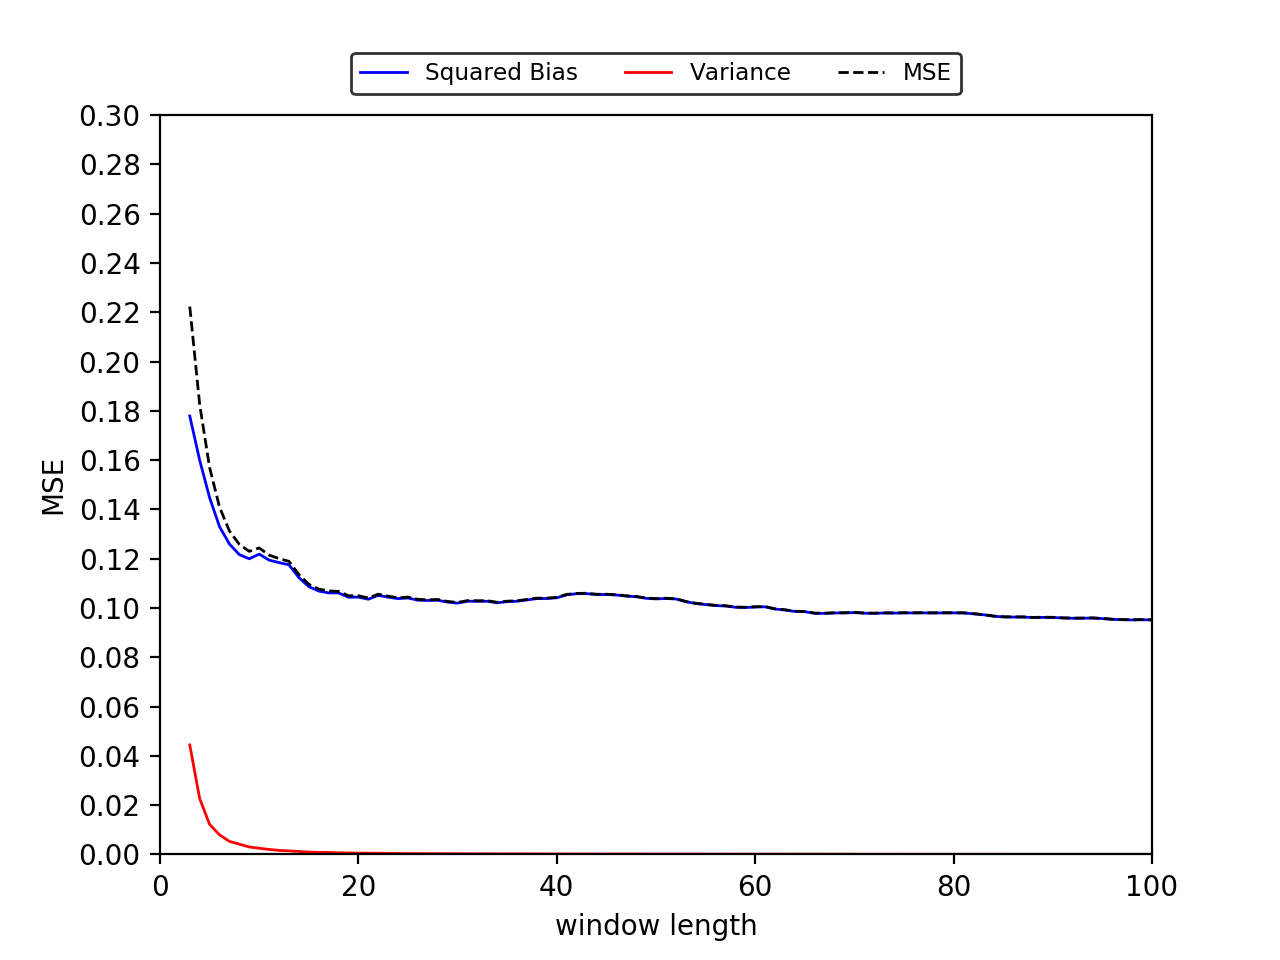
\includegraphics[width=\textwidth]{decom_mse_knn_kendall_proxy.png} 
		\caption{Bias-variance decomposition for KNN estimates with Kendall as covariate and proxy correlation.} 
		\label{fig:decom_mse_knn_kendall_proxy}
	\end{subfigure}
	\caption{MSE for KNN estimates with Pearson and Kendall Moving Window bootstrap estimates as covariates and proxy correlation.}
	\label{fig:decom_mse_knn5_pearson_kendall_proxy}
\end{figure}

\subsubsection{Alternative Parameterizations of Nearest Neighbor Algorithm}
Tabel \ref{tab:mse_decomp_knn_pearson_kendall_proxy} presents MSE decomposition as a function of number of neighbors $k$ for KNN estimates with approximations for both covariates and response variable. Similar results are observed for $k \in \{5, 10, 25, 50, 100\}$ when compared with KNN estimates with approximated covariates and true correlation in Tabel \ref{tab:mse_decomp_knn_pearson_kendall_true}; both squared bias and variance decrease with an increase in $k$, and conversely, regardless whether Pearson or Kendall estimates are used for defining the set of covariates. Given Eq. \eqref{eq:mse_decomposition_knn} and our discussion from Section \ref{sec:mse_decompose} one might have expected an increase in squared bias with an increase in $k$. A possible explanation for this behaviour may be that up to some $k$, an increase in $k$ implies additional neighbors containing informational value are used for the estimation of time-varying correlations. Logically, the inclusion of additional neighbors containing informational value results into more accurate estimates of correlation, i.e. a decrease in squared bias. As of some $k$, however, additional neighbors only add noise to the estimation process which results into increased squared bias. For KNN estimates with Kendall covariate and proxy correlation this is for $k = 900$ whereas squared bias still decreases for $k = 1000$ in the case of KNN estimates with Pearson covariate and proxy correlation. Given our discussion from Section \ref{sec:mse_decompose} and results from KNN estimates with approximated covariates and true correlation in Tabel \ref{tab:mse_decomp_knn_pearson_kendall_true}, one might have expected a continuing decrease in variance with an increase in $k$. Interestingly, Tabel \ref{tab:mse_decomp_knn_pearson_kendall_proxy} shows an increase in variance from $k = 800$ and $k = 900$ onwards for KNN estimates with Pearson and Kendall covariates, respectively.          


%% TABLE
\begin{table}[H]
\centering
\captionsetup[subtable]{position=below}
%\captionsetup[table]{position=below}
\begin{subtable}{0.49\linewidth}
\centering
\begin{tabular}{r  c  c  c} 
\toprule
\multicolumn{1}{ r }{\textbf{k}} &
\multicolumn{1}{ c }{\textbf{Squared Bias}} &
\multicolumn{1}{ c }{\textbf{Variance}} &
\multicolumn{1}{ c }{\textbf{MSE}} \\
\midrule 

5                                     & 0.1334                         & 0.0027                & 0.1361     \\
10                                   & 0.1319                         & 0.0015                & 0.1334     \\
25                                   & 0.1289 	                    & 6.64e-4                & 0.1295     \\
50                                   & 0.1268                         & 3.57e-4                & 0.1271     \\
100                                 & 0.1238                         & 1.95e-4               & 0.1240      \\
200                                 & 0.1169                         & 1.14e-4               & 0.1170      \\
400                                 & 0.1047                         & 7.80e-5               & 0.1048      \\
600                                 & 0.0946                         & 7.20e-5               & 0.0947     \\
800                                 & 0.0870                         & 7.50e-5               & 0.0870      \\
900				     & 0.0841			   & 8.00e-5              & 0.0842      \\
1000                               & 0.0827                         & 8.80e-5              & 0.0828     \\ [1ex]
\bottomrule
\end{tabular}
\caption{MSE for KNN estimates with window size 10, Pearson as covariate and correlation.}
\label{tab:mse_decomp_knn_pearson_proxy}
\end{subtable}
\hfill
\begin{subtable}{0.49\linewidth}
\centering
\begin{tabular}{r  c  c  c} 
\toprule
\multicolumn{1}{ r }{\textbf{k}} &
\multicolumn{1}{ c }{\textbf{Squared Bias}} &
\multicolumn{1}{ c }{\textbf{Variance}} &
\multicolumn{1}{ c }{\textbf{MSE}} \\
\midrule 

5                                     & 0.1219                         &  0.0025              & 0.1244   \\
10                                   & 0.1200                         & 0.0014               & 0.1214   \\
25                                   & 0.1183	                   & 5.98e-4              & 0.1189    \\
50                                   & 0.1168                        & 3.17e-4	       & 0.1171    \\
100                                 & 0.1148                         & 1.75e-4              & 0.1150    \\
200                                 & 0.1110                        & 1.02e-4              & 0.1110    \\
400                                 & 0.1042                        & 6.80e-5             & 0.1043   \\
600                                 & 0.0998                         & 6.00e-5             & 0.0998     \\
800                                 & 0.0969                         & 5.90e-5             & 0.0970    \\
900				     & 0.0969			   & 6.00e-5             & 0.0970     \\
1000                               & 0.0988                       & 6.30e-5             & 0.0988     \\  [1ex]
\bottomrule
\end{tabular}
\caption{MSE for KNN estimates with window size 10, Kendall as covariate and correlation.}
\label{tab:mse_decomp_knn_kendall_proxy}
\end{subtable}
\caption{Mean Squared Error (MSE) decomposition as a function of the number of neighbors (k) for KNN with approximations for both covariates and response variable.}
\label{tab:mse_decomp_knn_pearson_kendall_proxy}
\end{table}

\noindent
As in Section \ref{sec:knn_true_cor}, two more parameterizations of the KNN learning algorithm are analyzed where the set of neighbors used for point estimation of time-varying correlation is defined as the entire training set. The KNN algorithm uses an uniformly weighted average of correlations and an inverse distance weighted average of correlations, as defined in \eqref{eq:IDWfunction}, in the first and second parameterizations, respectively. However, the choice of an uniform distance weighting function results in approximately constant correlation, as depicted in Fig. \ref{fig:knn_pearson21_len_train_bootstrap_true} where the true correlation was considered as the response variable. The concept of assuming constant correlation is exactly what we are trying to improve on by considering correlation to be time-varying. As such, the remainder of this section will primarily focus on results from KNN estimates considering an inverse distance weighting function. \\
  
\noindent
Again, the accuracy of the two different parameterizations is compared by using mean squared error (MSE) between estimated and actual correlations. The MSE decomposition of KNN estimates under inverse distance weighting function and proxies for covariates and the response variable is depicted in Fig. \ref{fig:decom_mse_knn_IDW_pearson_kendall_proxy}. The variance term becomes negligible small in case the set of neighbors used for point estimation of time-varying correlation is defined as the entire training set. The red line of the variance is barely observable in the bottom of Fig. \ref{fig:decom_mse_knn_IDW_pearson_proxy}-\ref{fig:decom_mse_knn_IDW_kendall_proxy}. This is in line with results presented in Tabel \ref{tab:mse_decomp_knn_pearson_kendall_proxy} where the value of the variance term is negligible small for larger $k$, regardless whether the set of covariates is constructed from Pearson or Kendall moving window estimates of correlation. \\


\begin{figure}[H]  % [h] parameter makes sure figures are located at 'this' location.
	\centering
	\begin{subfigure}[b]{0.49 \textwidth}
		\centering 
		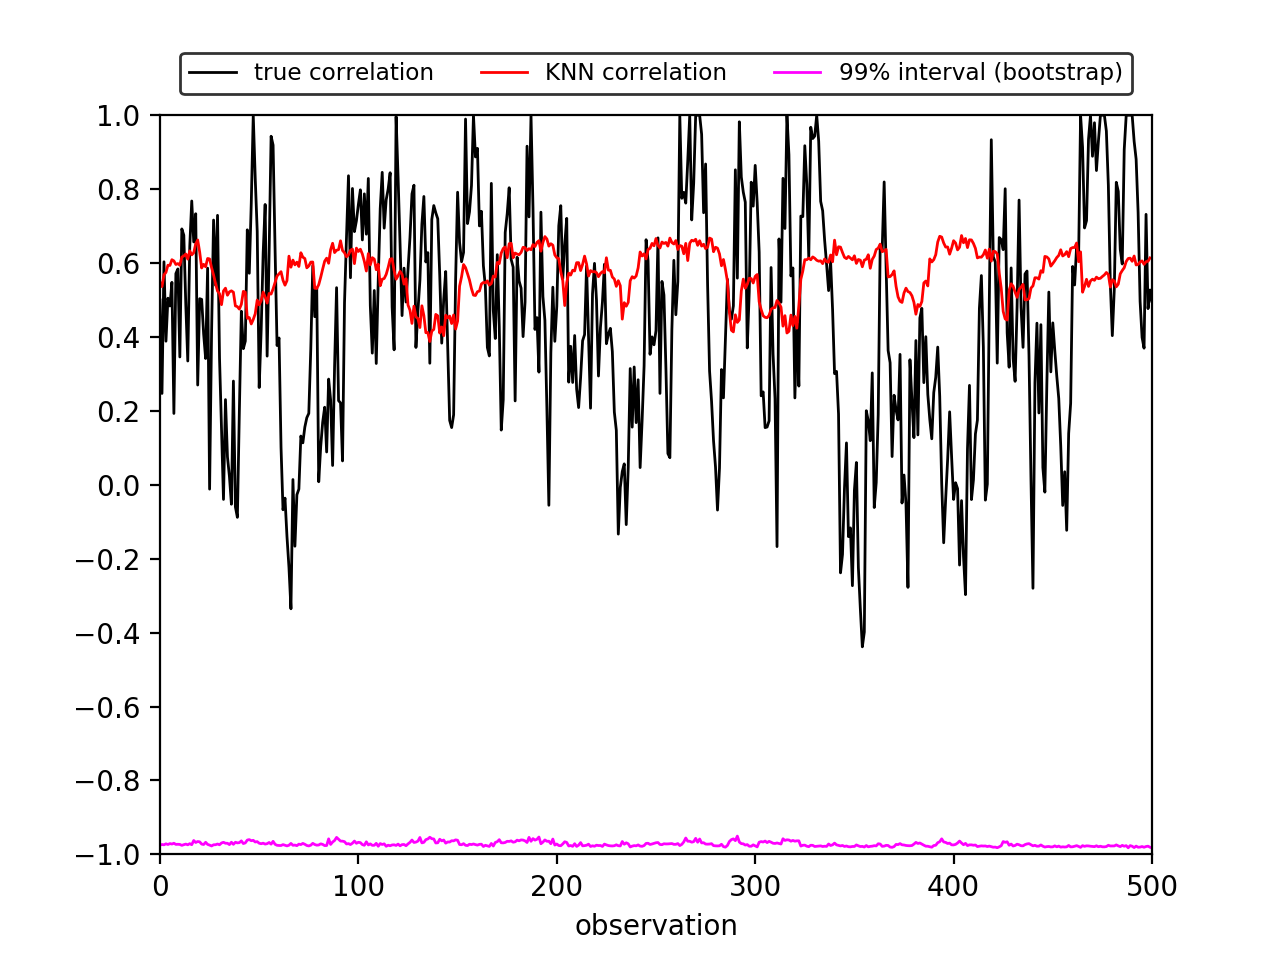
\includegraphics[width=\textwidth]{knn_pearson_21_IDW_estimates_bootstrap_proxy.png} 
		\caption{KNN estimates as inverse distance weighted averages, with window size 21 and Pearson covariates.} 	
		\label{fig:knn_pearson_21_IDW_estimates_bootstrap_proxy}
	\end{subfigure}
	\hfill  
	\begin{subfigure}[b]{0.49 \textwidth}
		\centering 
		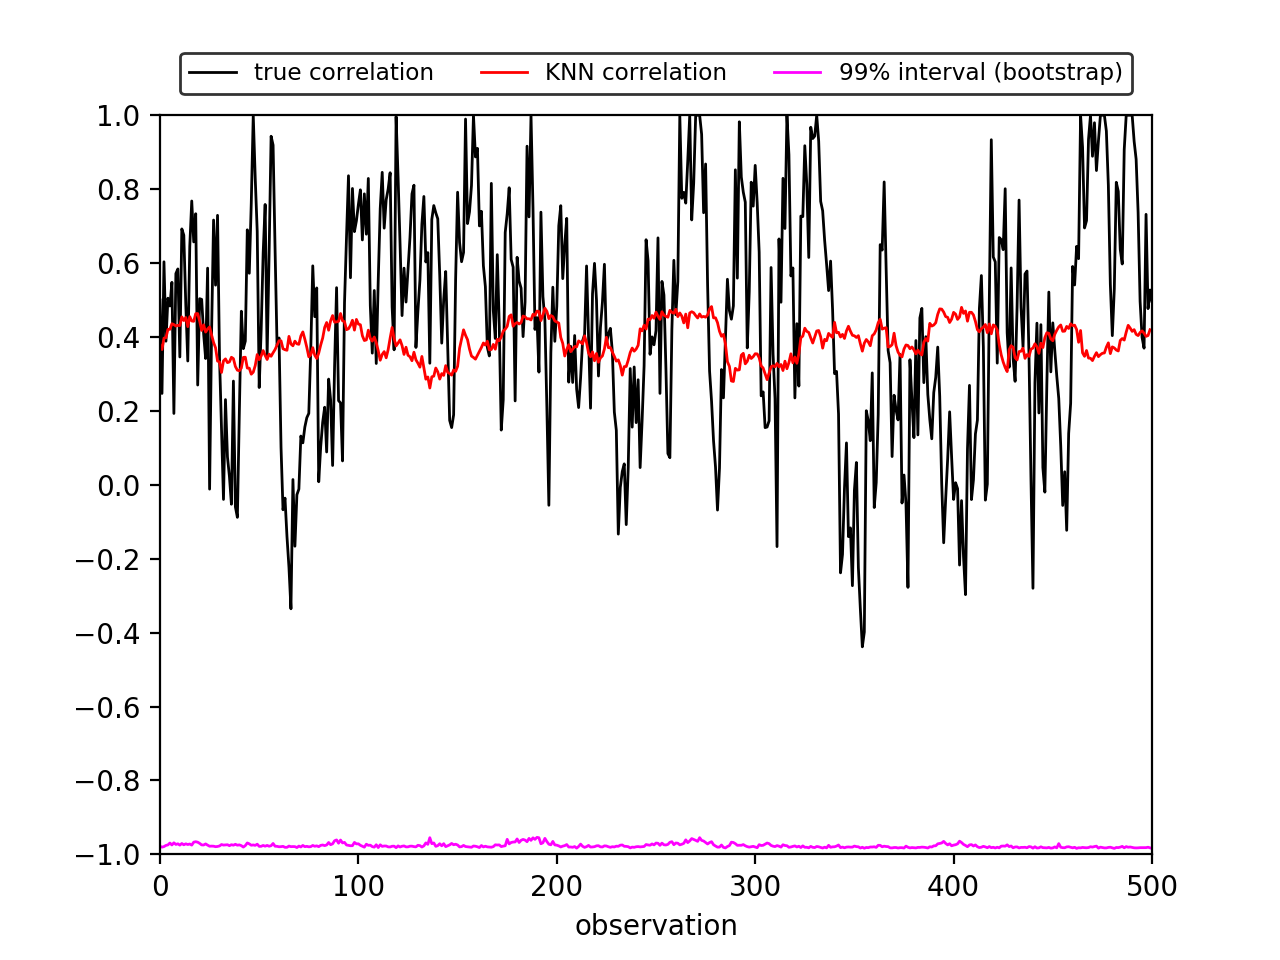
\includegraphics[width=\textwidth]{knn_kendall_21_IDW_estimates_bootstrap_proxy.png} 
		\caption{KNN estimates as inverse distance weighted averages, with window size 21 and Kendall covariates.} 
		\label{fig:knn_kendall_21_IDW_estimates_bootstrap_proxy}
	\end{subfigure}
	\hfill  
	\begin{subfigure}[b]{0.49 \textwidth}
		\centering 
		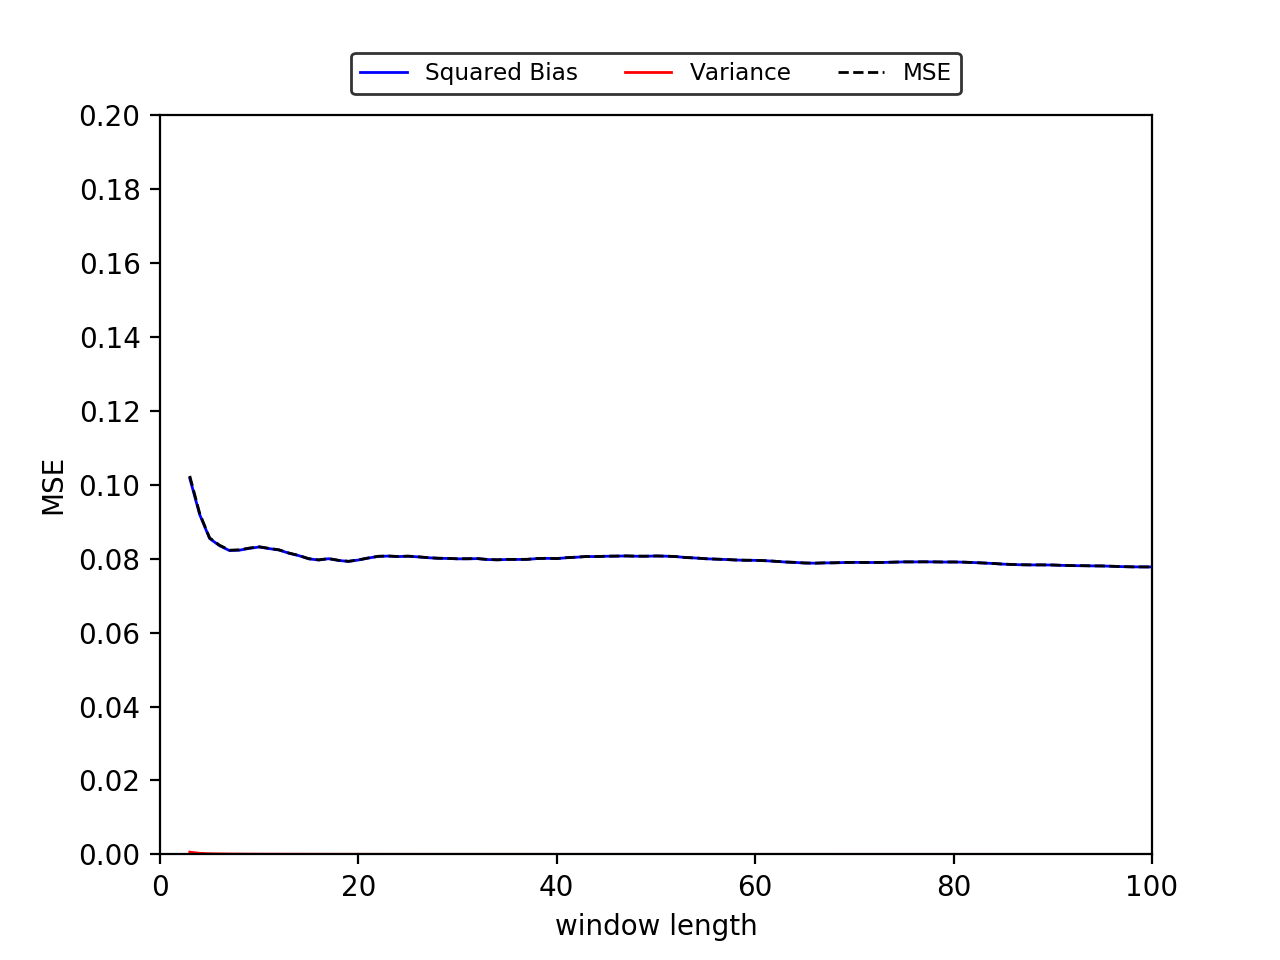
\includegraphics[width=\textwidth]{decom_mse_knn_IDW_pearson_proxy.png} 
		\caption{Bias-variance decomposition for KNN estimates constructed from inverse distance weighted averages and Pearson covariates.} 
		\label{fig:decom_mse_knn_IDW_pearson_proxy}
	\end{subfigure}
	\hfill  
	\begin{subfigure}[b]{0.49 \textwidth}
		\centering 
		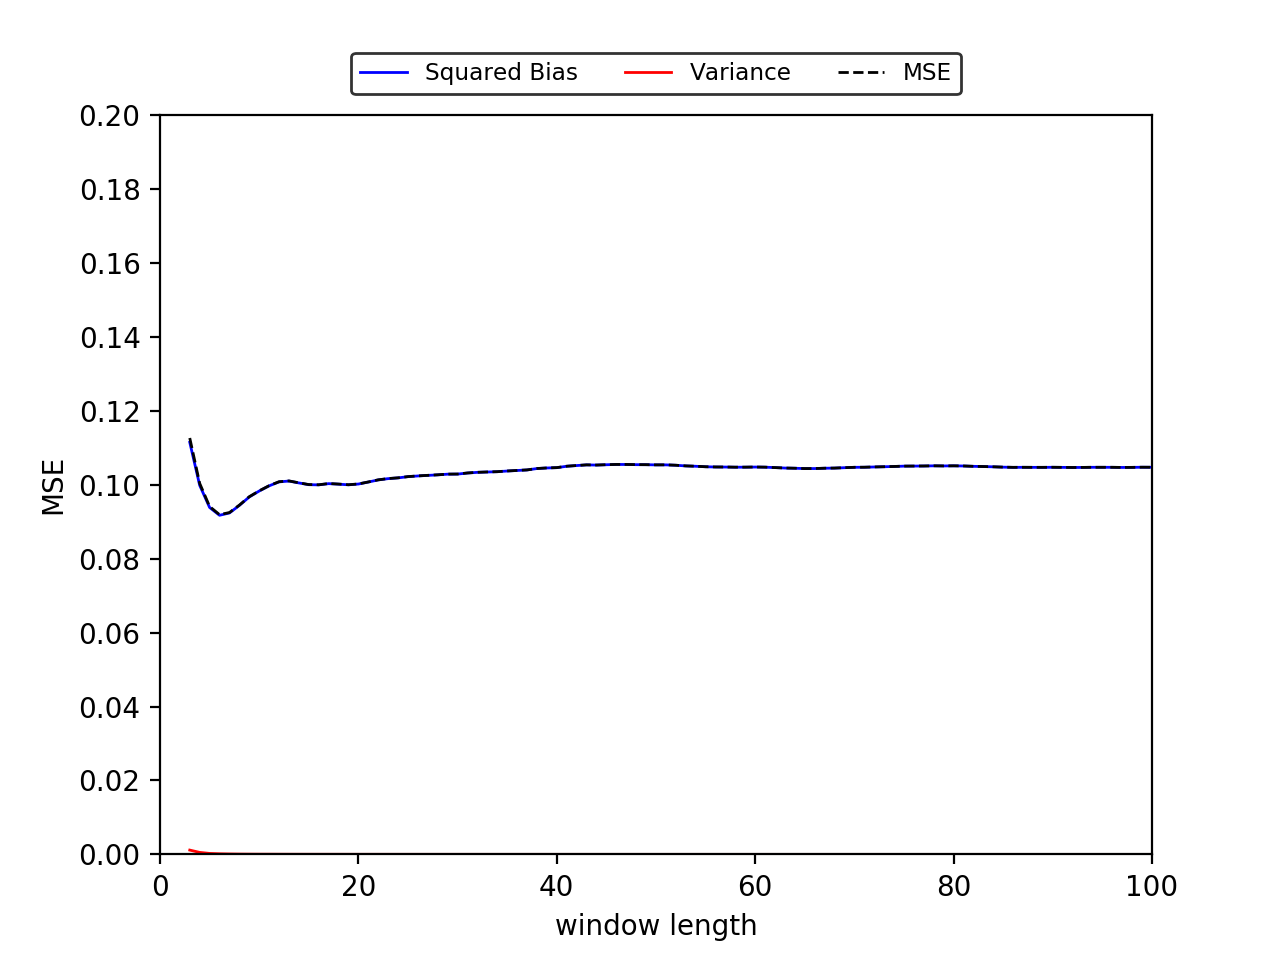
\includegraphics[width=\textwidth]{decom_mse_knn_IDW_kendall_proxy.png} 
		\caption{Bias-variance decomposition for KNN estimates constructed from inverse distance weighted averages and Kendall covariates.} 
		\label{fig:decom_mse_knn_IDW_kendall_proxy}
	\end{subfigure}
	\caption{MSE for KNN estimates with inverse weighting function, Pearson and Kendall Moving Window bootstrap estimates as covariates and response variable.}
	\label{fig:decom_mse_knn_IDW_pearson_kendall_proxy}
\end{figure}


\noindent
Regardless of the choice of window length, MSE from KNN with an uniform weighting function and the set of covariates and response variable constructed from Pearson and Kendall moving window estimates are approximately between 0.0774 and 0.0923, and 0.1054 and 0.1118, respectively. 
MSE from KNN with an inverse distance weighting function is approximately between 0.0778 and 0.1024, and between 0.0919 and 0.1127 when Pearson and Kendall moving window estimates are used as covariates and response variable, respectively. This implies that Pearson moving window estimates as covariates and approximation of true correlation in KNN seems more appropriate for the simulated data than Kendall moving window estimates, regardless of the weighting function; Fig. \ref{fig:decom_mse_knn_IDW_pearson_proxy} depicts a lower MSE for all window sizes compared with MSE in Fig. \ref{fig:decom_mse_knn_IDW_kendall_proxy}. An explanation for this observation is given along the same lines as for Pearson and Kendall moving window estimates in Section \ref{sec:true_correlation}; the simulated asset returns follow a multivariate normal distribution, i.e. an elliptical distribution. Therefore, it makes sense that lower MSE values are obtained when true correlation in KNN is approximated using a linear correlation coefficient such as Pearson. Moreover, the choice for an inverse distance weighting function seems to have no real performance advantage over an uniform weighting function when true correlation is approximated using moving window estimates and MSE serves as the performance measures MSE. Interestingly, this is in contrast with results obtained from KNN estimates with true correlation in Section \ref{sec:knn_true_cor}. More importantly however, using a uniform weighting function with the entire training set results in approximately constant correlation, which is the exact concept we are intending to improve with a more realistic assumption of time-varying correlation. The latter is better captured under an inverse distance weighting function. Finally, the variance of MSE from KNN with uniform weighting function and the set of covariates constructed from Pearson and Kendall moving window estimates are approximately 3.98e-6 and 9.26e-7, respectively. The variance of MSE from KNN with inverse distance weighting function and the set of covariates constructed from Pearson and Kendall moving window estimates are approximately 8.46e-6 and 8.61e-6, respectively. The difference in sensitivity to the choice of window length between the different parameterizations is negligible small if significant at all. \\


\noindent
The alternative parameterizations of the KNN algorithm with approximated covariates and response variable also satisfy the positive semi-definiteness condition in the time-varying correlation matrix $R_t$ for all time $t$ under all choices of window length in the interval [0, 100]. Fig. \ref{fig:det_knn_len_train_IDW_pearson_kendall_proxy} presents the obtained minimum determinants of $R_t$ for all choices of window length under the proposed alternative parameterizations.\\

\noindent 
Similar to Section \ref{sec:knn_true_cor}, this section is concluded with a comparison of the function approximation capabilities of the KNN algorithm and Pearson and Kendall moving window estimates. The comparison is based on MSE between estimated and actual correlations. Fig. \ref{fig:mse_knn5_IDW_pearson_kendall_proxy} shows MSE from KNN with default parameterizations, i.e. number of neighbors equals 5, an alternative parameterizations with an inverse distance weighting function and the full training set used for estimating time-varying correlations. Additionally Pearson and Kendall moving window estimates of time-varying correlations are shown. According to MSE, parameterizations of the KNN algorithm with approximated covariates and response variable performs significantly better than those of Pearson and Kendall moving window estimates for small window sizes. Moreover, parameterizations of the KNN algorithm with an alternative distance weighting function and full use of training data set results in significantly smaller MSE compared to Pearson and Kendall moving window estimates for all window sizes. Thus, similar to the analysis in Section \ref{sec:knn_true_cor}, KNN estimates with an increase in the number of neighbors have lower MSE, particularly for smaller window sizes. This result follows from the fact that time-varying correlations are then estimated using increased sample information, which positively contributes to accurately capturing time variation in correlations. Finally, the variance of MSE from KNN estimates with default parameterizations and with the combination of an inverse distance weighting function and use of full training set in Fig. \ref{fig:mse_knn5_IDW_pearson_kendall_proxy} are 5.70e-4 and 8.46e-6, respectively, while that of Pearson and Kendall moving window estimates are 0.0040 and 0.0037, respectively. In other words, the KNN algorithm with approximated covariates and response variable is significantly less sensitive to the choice of window length than Pearson and Kendall moving window estimates of correlation.  \\

\begin{figure}[H] 
	\centering
	\begin{subfigure}[b]{0.49 \textwidth}
		\centering 
		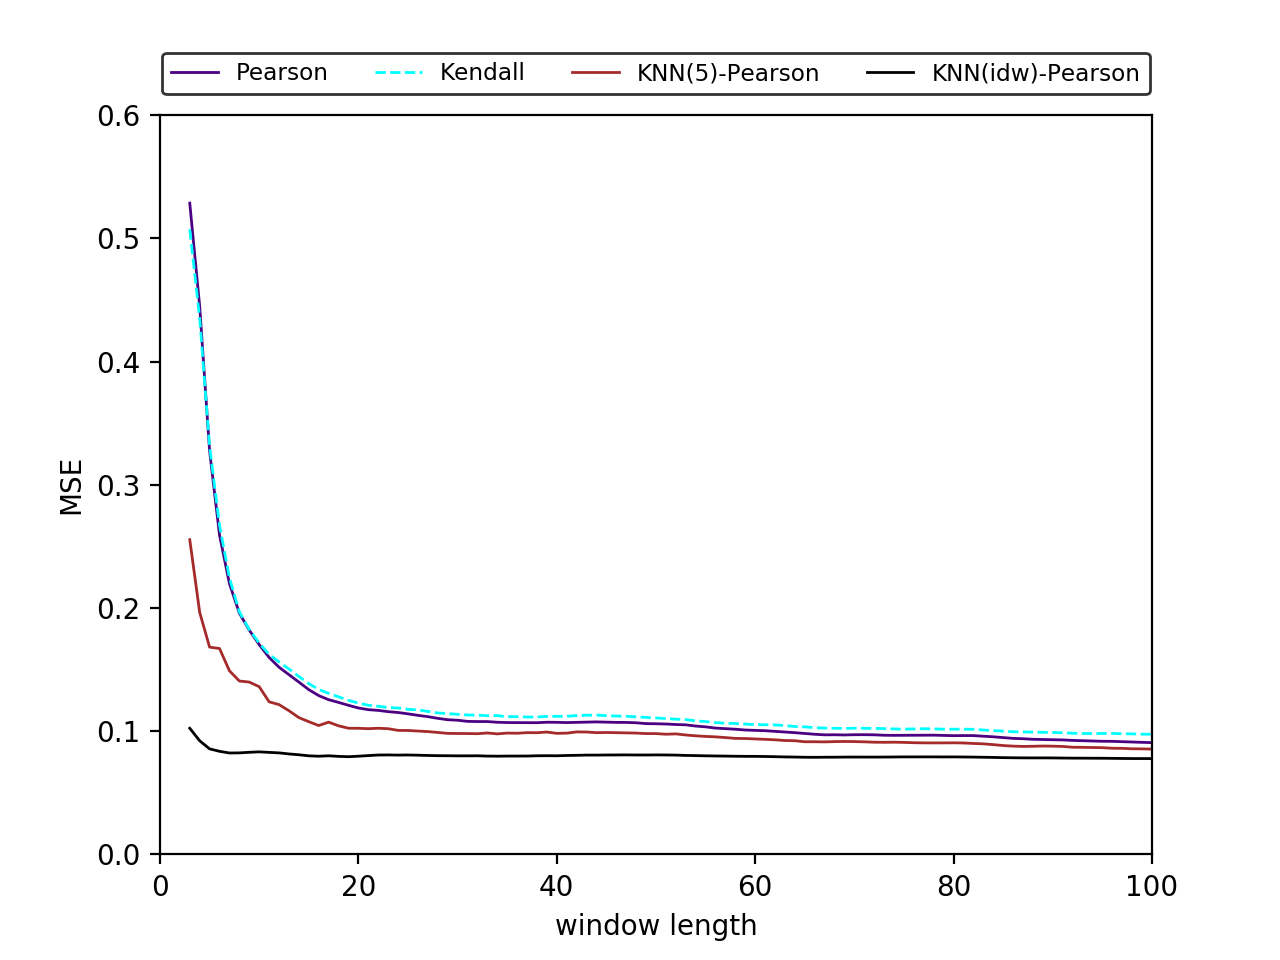
\includegraphics[width=\textwidth]{mse_knn5_IDW_pearson_kendall_proxy} 
		\caption{MSE for KNN with Pearson covariates and proxy correlation, Pearson and Kendall Moving Window bootstrap estimates.}
		\label{fig:mse_knn5_IDW_pearson_kendall_proxy}
	\end{subfigure}
	\hfill
	\begin{subfigure}[b]{0.49 \textwidth} 
		\centering
		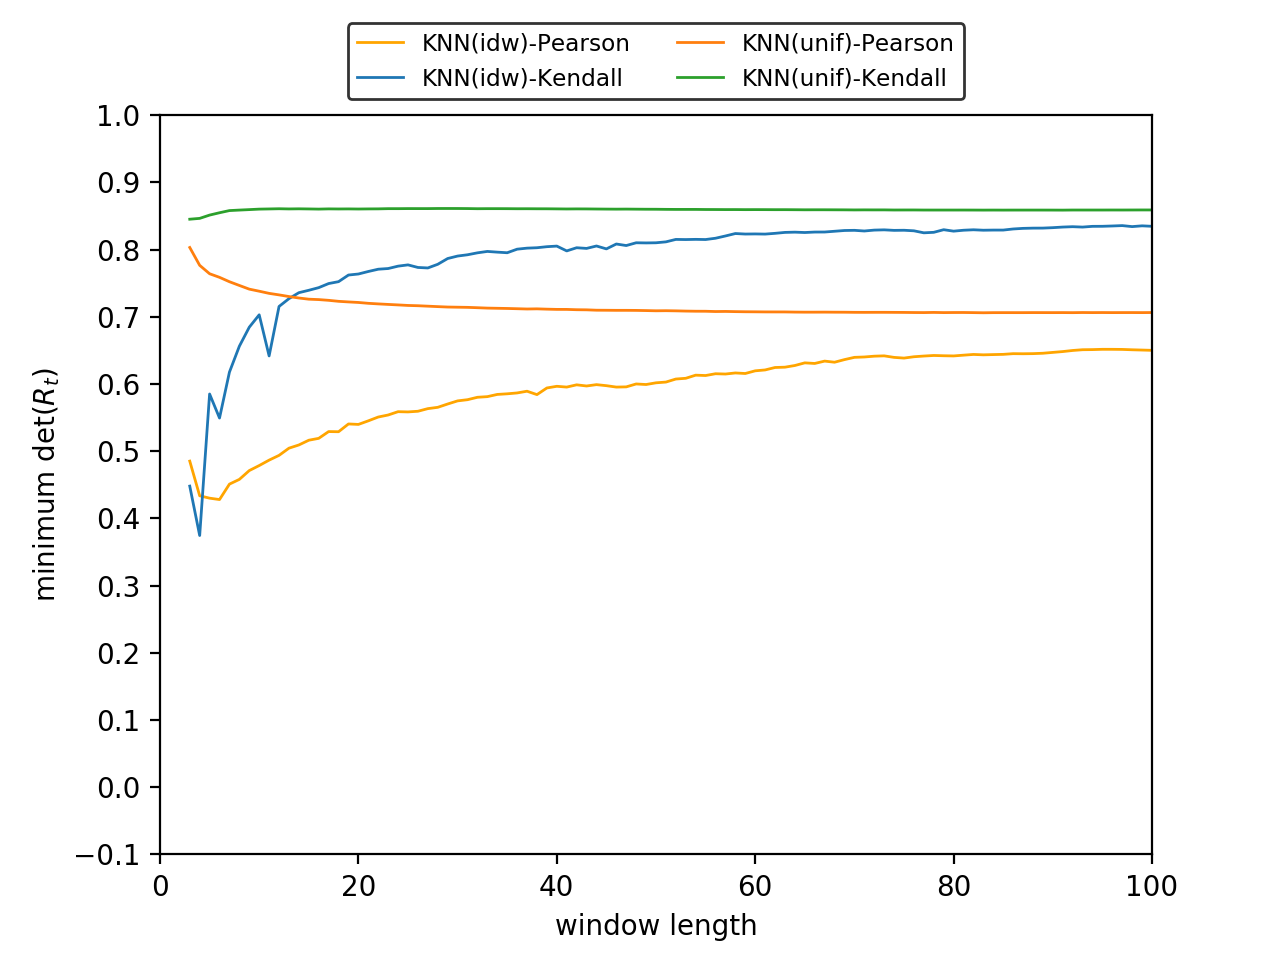
\includegraphics[width=\textwidth]{det_knn_IDW_len_train_pearson_kendall_proxy}
		\caption{Minimum determinants for KNN using uniform and inverse distance weighting function, Pearson and Kendall covariates and proxy correlation.}
		\label{fig:det_knn_len_train_IDW_pearson_kendall_proxy}
	\end{subfigure}	
	\caption{Comparison MSE and minimum determinants for KNN with Pearson covariates and proxy correlation, Pearson and Kendall Moving Window bootstrap estimates.}
	\label{mse_det_knn5_IDW_pearson_kendall_proxy}
\end{figure}







%%%%%%% RANDOM FOREST PROXY %%%%%%%%%%%%%%
\subsection{Random Forest} \label{sec:rf_proxy_cor}
In order to obtain time-varying correlations, $\rho_t$, with random forests algorithm, the set of covariates is defined by lagged Pearson and Kendall moving window estimates and minimum and maximum log return from the last period, denoted by $min_{i}(r_{i,t-1})$, and $max_{i}(r_{i,t-1})$, respectively.  \\

\subsubsection{Diagnosing the Generalization Error of Random Forest}
The accuracy of RF estimates with Pearson and Kendall covariates for time-varying correlation is compared by using mean squared error (MSE) between estimated and actual correlations. MSE from RF with Pearson and Kendall moving window estimates of correlation for covariates and as response variable are shown in Fig. \ref{fig:mse_rf10_pearson_kendall_proxy}. Regardless of the choice of window length, MSE from RF with Pearson and Kendall covariates are between 0.0868 and 0.2318, and 0.0946 and 0.2321, respectively. The variance of MSE from RF estimates with Pearson covariates is approximately 4.54e-4 while that of RF estimates with Kendall covariates is approximately 3.23e-4. Interestingly, Fig. \ref{fig:mse_rf10_pearson_kendall_proxy} shows that MSE from RF estimation with Pearson or Kendall approximations for the response variable varies substantially for smaller window sizes. Although, less variation is observed when compared with MSE from Pearson and Kendall moving window estimates depicted in Fig. \ref{fig:mse_pearson_kendall_bootstrap}. This observation is analogous to the comparison of KNN estimates of correlation for both true correlation and approximated correlation as response variable. \\

\noindent
Moreover, RF estimates of time-varying correlation where both the set of covariates and response variable is constructed from Pearson and Kendall moving window estimates satisfy the positive semi-definiteness condition in the time-varying correlation matrix $R_t$ for all time $t$ under all considered choices of window length. Fig. \ref{fig:det_rf10_pearson_kendall_proxy} presents the obtained minimum determinants of $R_t$ for all choices of window length. Although the minimum determinants for smaller window sizes approach 0, they remain nonnegative for all time $t$.

\begin{figure}[H]
	\centering
	\begin{subfigure}[b]{0.49 \textwidth} 
		\centering
		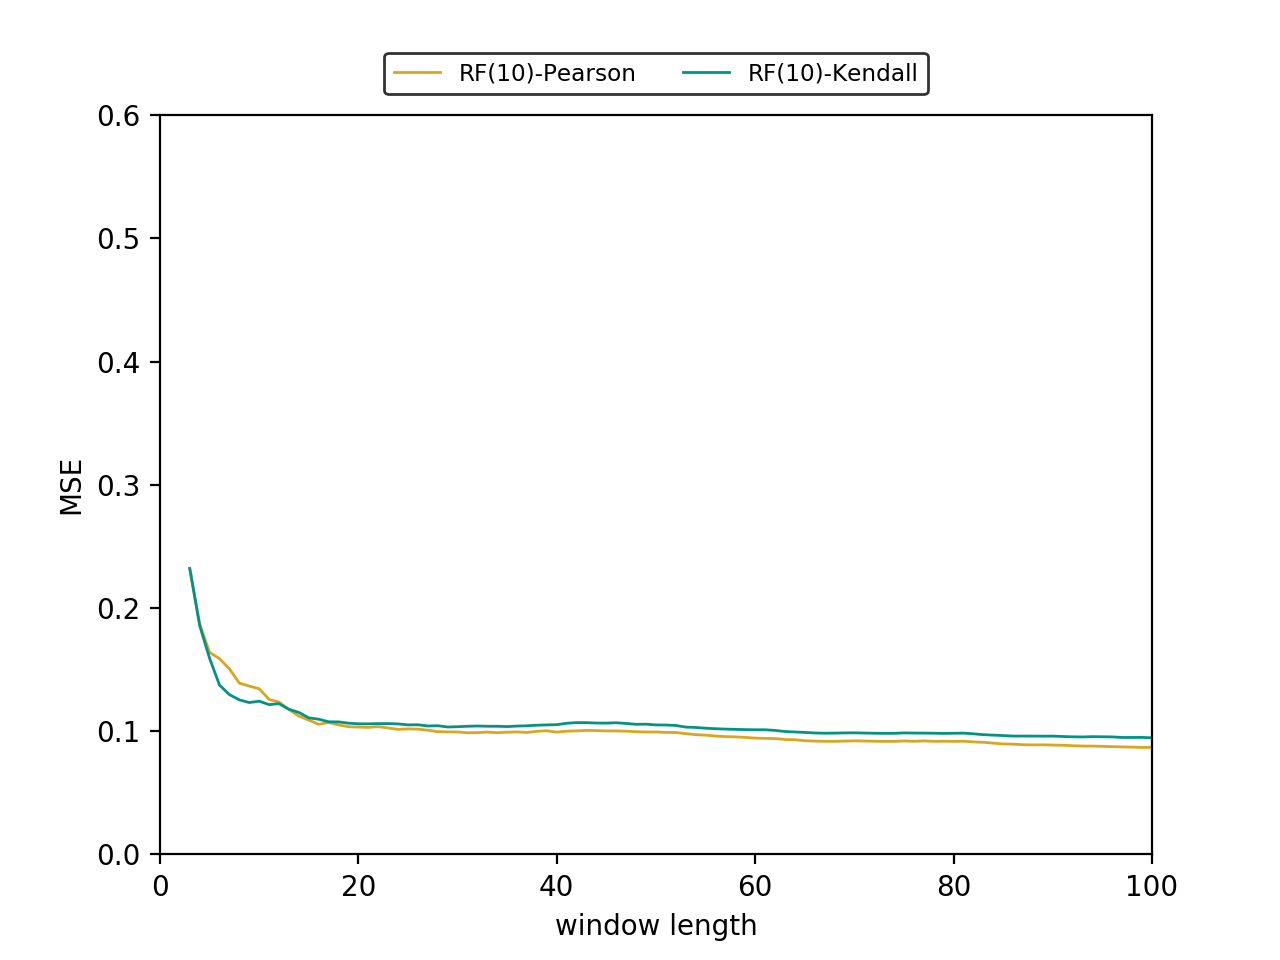
\includegraphics[width=\textwidth]{mse_rf10_pearson_kendall_proxy}
		\caption{MSE for RF with covariates from Pearson and Kendall and proxy correlation.}
		\label{fig:mse_rf10_pearson_kendall_proxy}
	\end{subfigure}
	\hfill
	\begin{subfigure}[b]{0.49 \textwidth} 
		\centering
		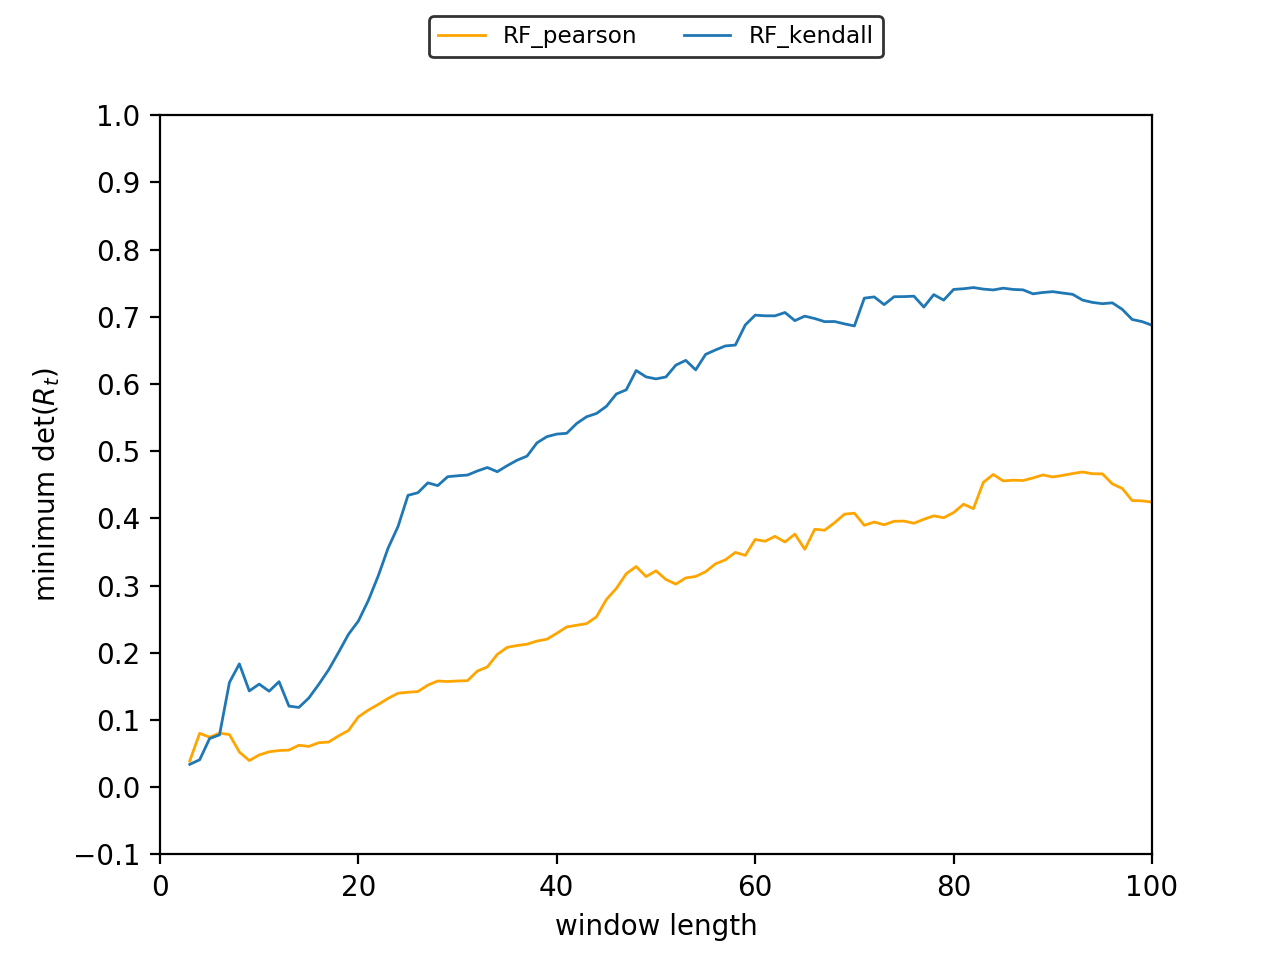
\includegraphics[width=\textwidth]{det_rf10_pearson_kendall_proxy}
		\caption{Minimum determinants for RF with covariates from Pearson and Kendall and proxy correlation.}
		\label{fig:det_rf10_pearson_kendall_proxy}
	\end{subfigure}
	\caption{Comparison MSE and minimum determinants for RF(n\_estimators=10) with covariates from Pearson and Kendall and proxy correlation.}
	\label{fig:mse_det_rf10_pearson_kendall_proxy}
\end{figure}

\noindent
A visual inspection of the plots in Fig. \ref{fig:rf_pearson21_bootstrap_proxy} and Fig. \ref{fig:rf_kendall21_bootstrap_proxy} results in an analysis that is analogous to the analysis of KNN estimates with approximations of correlation instead of actual correlation in Section \ref{sec:knn_proxy_cor}. It is clear that the uncertainty in the time-varying correlation $\rho_t$, which is illustrated by the 99\% confidence interval, is smaller for RF estimates compared to Pearson moving window estimates and Kendall moving window estimates, even though both the set of covariates and the response variable of the RF algorithm are based on approximations of correlation instead of actual correlation. These figures also show smaller uncertainty in the time-varying correlation $\rho_t$ when compared with RF estimates with true correlation as the response variable, which are depicted in Fig. \ref{fig:decom_mse_rf10_pearson_kendall_true}; RF estimates of correlation with true correlation as response variable in Fig. \ref{fig:rf_pearson21_bootstrap_true} and Fig. \ref{fig:rf_kendall21_bootstrap_true} are much more volatile. RF estimates with approximated correlation as response variable in Fig. \ref{fig:rf_pearson21_bootstrap_proxy} and Fig. \ref{fig:rf_kendall21_bootstrap_proxy} , however, follow the increases and decreases of the actual correlation smoother, with tighter confidence intervals. This is a more desirable result as it is not expected that correlation between assets changes that drastically at each time unit. \\

\noindent
The MSE decompositions into bias and variance terms from RF estimates of correlation are shown in Fig. \ref{fig:rf_pearson21_bootstrap_proxy} and Fig. \ref{fig:decom_mse_rf10_pearson_proxy}. These figures indicate that the RF algorithm with approximated output is more sensitive to the choice of the window length for smaller window sizes compared to RF algorithm with true correlation depicted in Fig. \ref{fig:decom_mse_rf10_pearson_kendall_true}. This observation is similar to the observation when comparing the KNN algorithm with different outputs and can be explained by error propagation: the effect of covariates' uncertainties (or errors) on the error of the function based on them. In the case when the RF algorithm uses proxies for response variables, the error associated with approximation of true correlation using moving window estimates is propagated to the output of the RF algorithm. Fig. \ref{fig:decom_mse_rf10_pearson_proxy} and Fig. \ref{fig:decom_mse_rf10_kendall_proxy} show, however, that the RF algorithm with approximated output is considerably less sensitive to the choice of the window length for smaller window sizes when compared to Pearson and Kendall moving window estimates of correlation depicted in Fig. \ref{fig:decom_mse_pearson}  and Fig \ref{fig:decom_mse_kendall}, respectively. Thus, analogous to the KNN algorithm with approximated covariates and response variable, the RF algorithm seems to mitigate the error propagation to some extend for smaller window sizes. A lower bias compared to Pearson and Kendall moving window estimates of correlation implies random forests may be a more suitable model for modeling time-varying correlations. Additionally, lower variance is observed when compared with Pearson and Kendall moving window estimates of correlation. This can be accredited to the the bootstrap aggregating method underlying the RF algorithm.       



\begin{figure}[H]  % [h] parameter makes sure figures are located at 'this' location.
	\centering
	\begin{subfigure}[b]{0.49 \textwidth} % sum of widths should be less than text width if all one the same line
		\centering 
		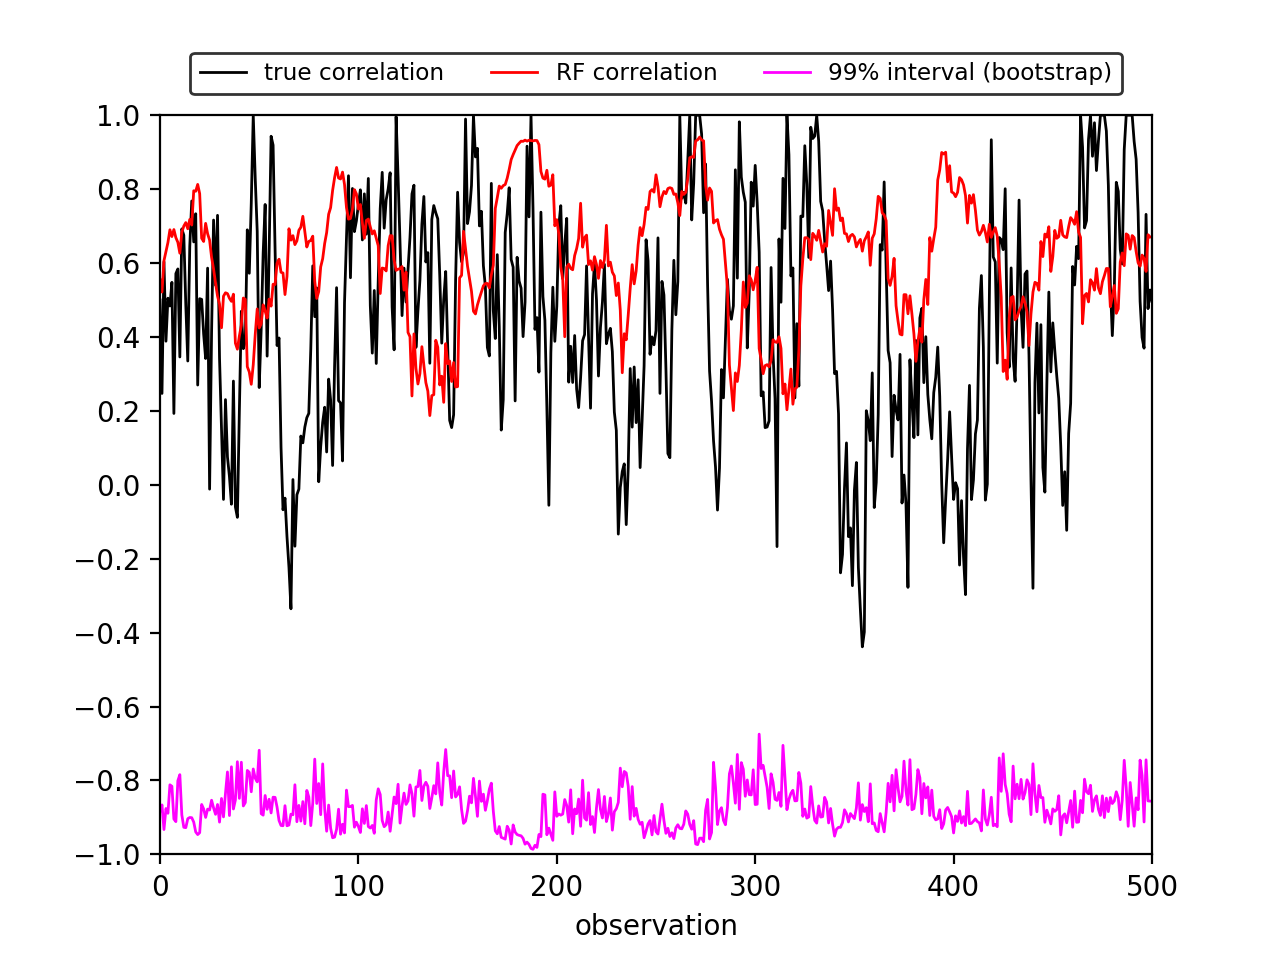
\includegraphics[width=\textwidth]{rf_pearson_21_estimates_bootstrap_proxy.png} 
		\caption{RF estimates with window size 21, Pearson as covariate and proxy correlation.} 	
		\label{fig:rf_pearson21_bootstrap_proxy}
	\end{subfigure} 
	\hfill	
	\begin{subfigure}[b]{0.49 \textwidth} 
		\centering 
		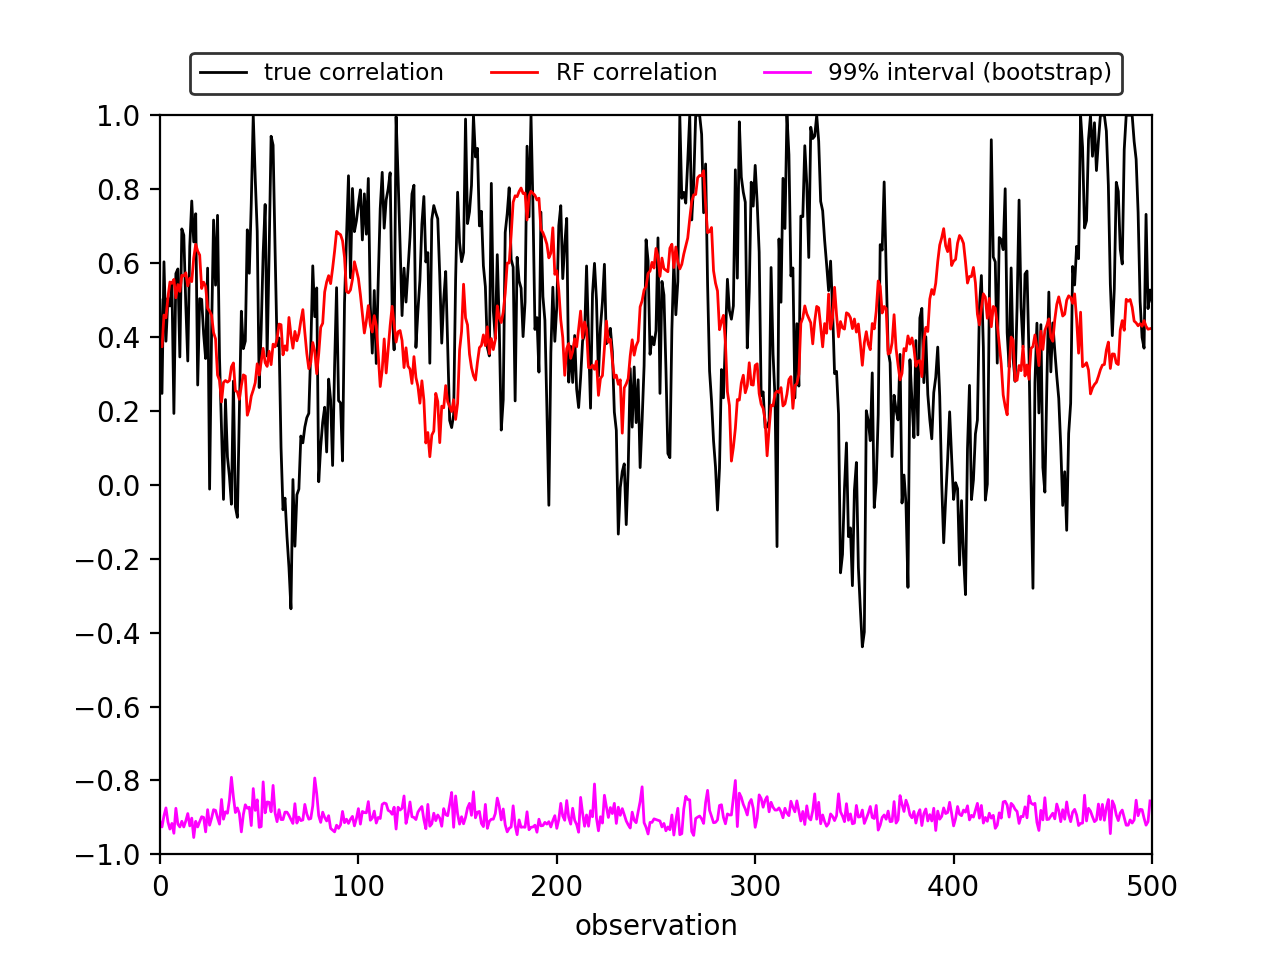
\includegraphics[width=\textwidth]{rf_kendall_21_estimates_bootstrap_proxy.png} 
		\caption{RF estimates with window size 21, Kendall as covariate and proxy correlation.} 
		\label{fig:rf_kendall21_bootstrap_proxy}
	\end{subfigure} 
	\hfill	
	\begin{subfigure}[b]{0.49 \textwidth}
		\centering 		
		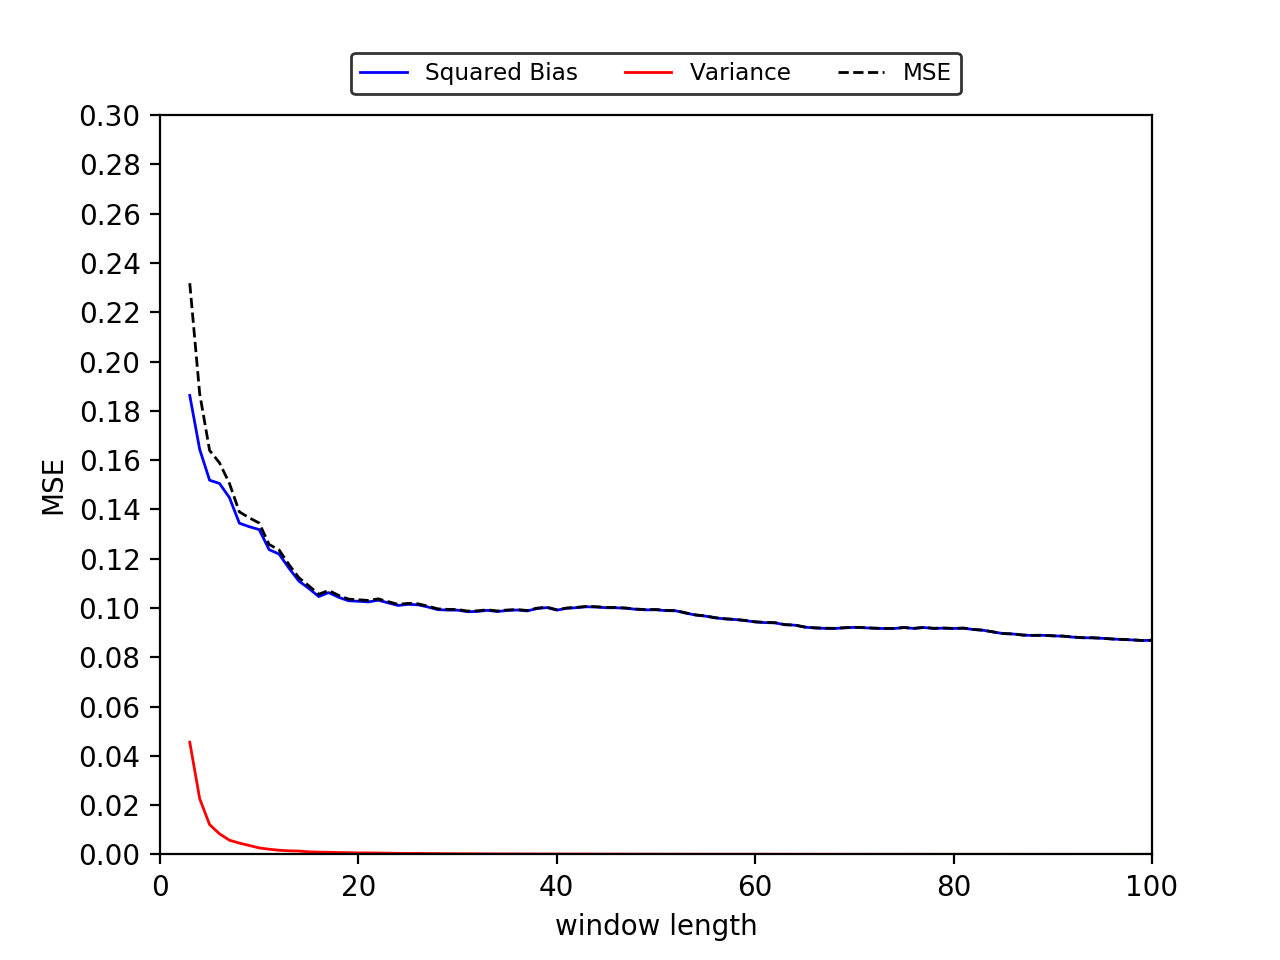
\includegraphics[width=\textwidth]{decom_mse_rf10_pearson_proxy.png} 
		\caption{Bias-variance decomposition for RF estimates with Pearson as covariate and proxy correlation.} 
		\label{fig:decom_mse_rf10_pearson_proxy}
	\end{subfigure}
	\hfill  
	\begin{subfigure}[b]{0.49 \textwidth}
		\centering 
		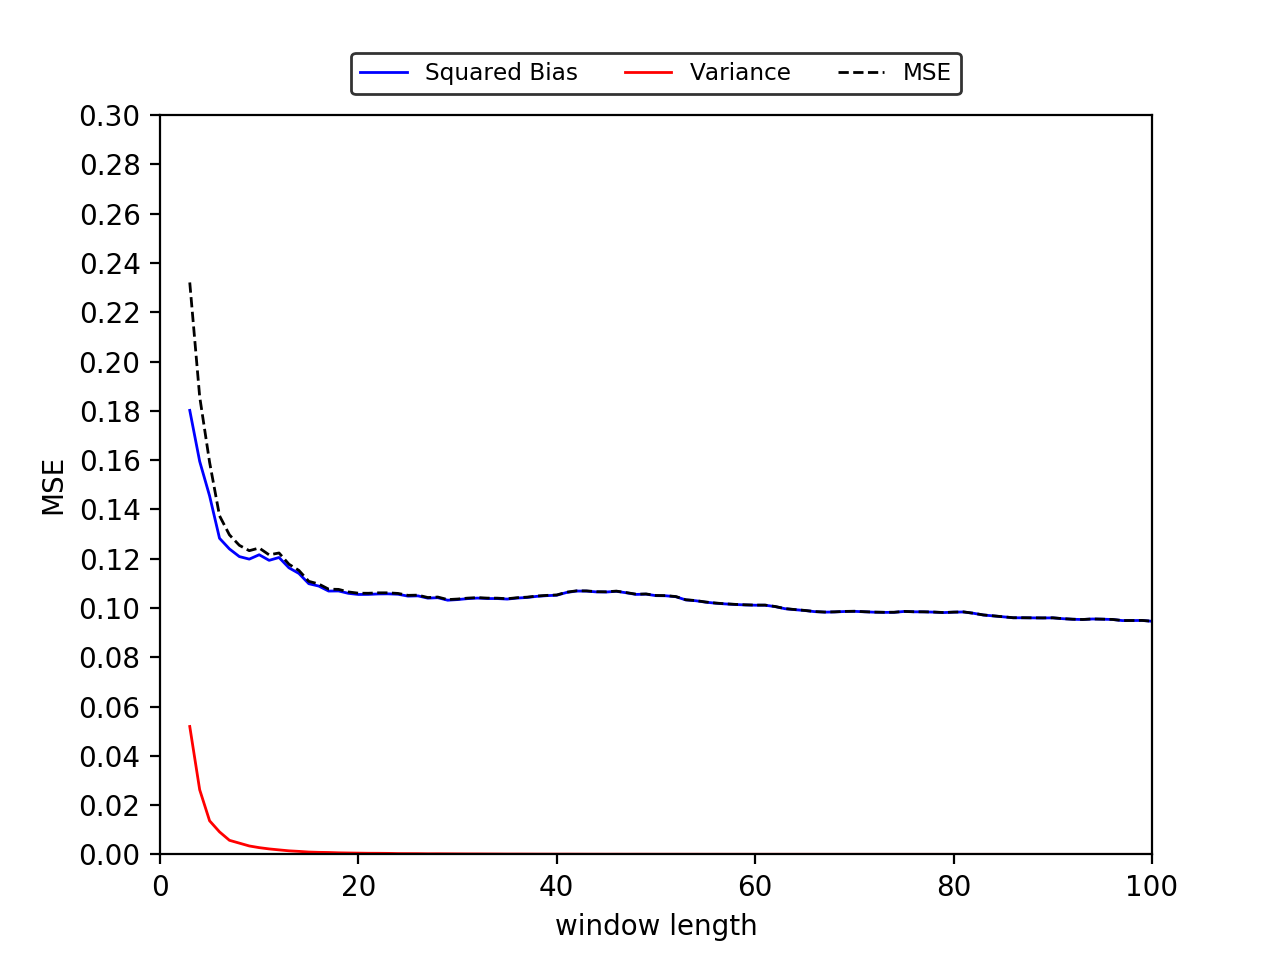
\includegraphics[width=\textwidth]{decom_mse_rf10_kendall_proxy.png} 
		\caption{Bias-variance decomposition for RF estimates with Kendall as covariate and proxy correlation.} 
		\label{fig:decom_mse_rf10_kendall_proxy}
	\end{subfigure}
	\caption{MSE for RF estimates with Pearson and Kendall Moving Window bootstrap estimates as covariates and proxy correlation.}
	\label{fig:decom_mse_rf10_pearson_kendall_proxy}
\end{figure}

\subsubsection{Alternative Parameterizations of Random Forest Algorithm}
\textbf{State that we take 100 bootstrapped samples instead of 1000 due to time constraints. This number of bootstrapped samples will however be sufficient for illustrational purposes.} \\

\noindent
Simulation results in Tabel \ref{tab:mse_decomp_rf_pearson_kendall_proxy} show an inverse relationship between the choice of the number of estimators (trees) in the random forest used for estimation of correlations and the uncertainty around the estimated correlations, regardless whether Pearson or Kendall estimates are used for defining the set of covariates. It is clearly observed that an increase in the number of estimators results in a decrease of the variance, and conversely. This observation is in line with our discussion on MSE decomposition for the RF algorithm and Eq. \eqref{eq:variance_rf} from Section \ref{sec:mse_decompose}. For this particular dataset it is observed that the point of diminishing reduction in variance is reached with a smaller amount of trees compared with the sensitivity analysis of the random forest that has true correlation as the response variable.  \\  




%% TABLE
\begin{table}[H]
\centering
\captionsetup[subtable]{position=below}
%\captionsetup[table]{position=below}
\begin{subtable}{0.49\linewidth}
\centering
\begin{tabular}{r  c  c  c} 
\toprule
\multicolumn{1}{ r }{\textbf{Trees}} &
\multicolumn{1}{ c }{\textbf{Squared Bias}} &
\multicolumn{1}{ c }{\textbf{Variance}} &
\multicolumn{1}{ c }{\textbf{MSE}} \\
\midrule 

10                                   &   0.1318                       & 0.0026                & 0.1344      \\
100                                 & 0.1320                         & 0.0016               & 0.1335       \\
300                                 & 0.1317                         & 0.0015               & 0.1333       \\
600                                 & 0.1320                         & 0.0015               & 0.1335     \\
1000                               & 0.1319                         &  0.0015              & 0.1334     \\ [1ex]

\bottomrule
\end{tabular}
\caption{MSE for RF estimates with window size 10, Pearson as covariate and correlation.}
\label{tab:mse_decomp_rf_pearson_proxy}
\end{subtable}
\hfill
\begin{subtable}{0.49\linewidth}
\centering
\begin{tabular}{r  c  c  c} 
\toprule
\multicolumn{1}{ r }{\textbf{Trees}} &
\multicolumn{1}{ c }{\textbf{Squared Bias}} &
\multicolumn{1}{ c }{\textbf{Variance}} &
\multicolumn{1}{ c }{\textbf{MSE}} \\
\midrule 

10                                   & 0.1217                         & 0.0027               &  0.1244      \\
100                                 & 0.1219                          & 0.0018               & 0.1236       \\
300                                 & 0.1215                         & 0.0017               &  0.1232      \\
600                                 & 0.1217                         & 0.0017               & 0.1234     \\
1000                               &  0.1214                         &   0.0017             &  0.1230     \\ [1ex]

\bottomrule
\end{tabular}
\caption{MSE for RF estimates with window size 10, Kendall as covariate and correlation.}
\label{tab:mse_decomp_rf_kendall_proxy}
\end{subtable}
\caption{Mean Squared Error (MSE) decomposition as a function of the number of estimators (trees) for RF with approximations for both covariates and response variable.}
\label{tab:mse_decomp_rf_pearson_kendall_proxy}
\end{table}

\noindent
\textbf{Insert sensitivity  analysis where MSE is a function of number of covariates used in the tree construction process of random forest algorithm.} \\

\noindent
This section is concluded with a comparison of the function approximation capabilities of the RF algorithm and Pearson and Kendall moving window estimates. The comparison is based on MSE between estimated and actual correlations. Fig. \ref{fig:mse_rf10_pearson_kendall_comp_proxy.png} shows MSE from RF with default parameterization, i.e. number of estimators equals 10, as well as Pearson and Kendall moving window estimates of time-varying correlations. According to MSE, default parameterizations of the RF algorithm results in significantly smaller MSE compared to Pearson and Kendall moving window estimates for smaller window sizes. Finally, the variance of MSE from RF estimates with default parameterization and Pearson and Kendall approximations of true correlation in Fig. \ref{fig:mse_rf10_pearson_kendall_comp_proxy.png} are 4.54-4 and 3.23e-4, respectively, while that of Pearson and Kendall moving window estimates are 0.0040 and 0.0037, respectively. \\


\begin{figure}[H]
	\centering
	\begin{subfigure}[b]{0.49 \textwidth} 
		\centering
		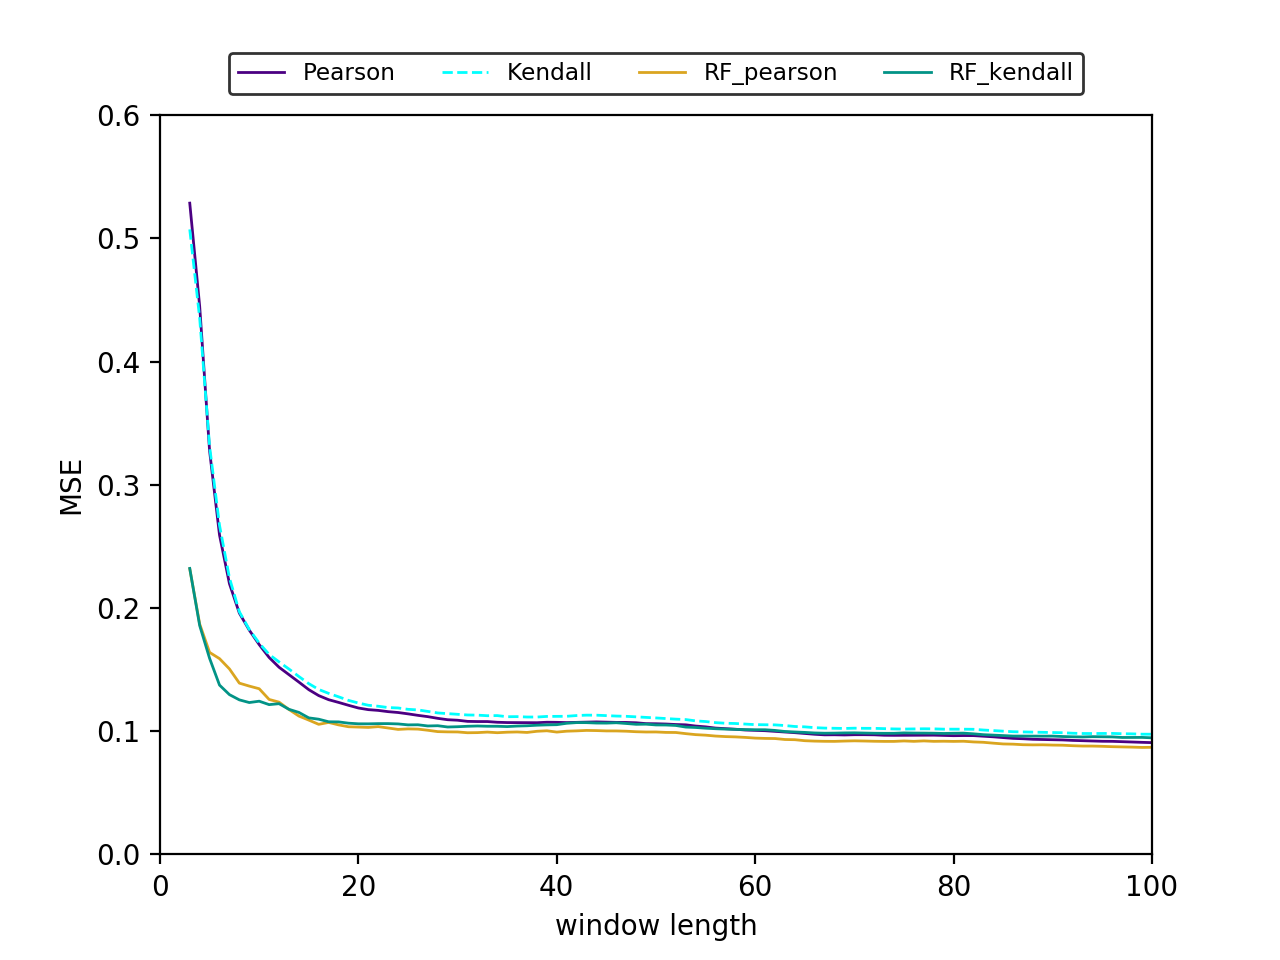
\includegraphics[width=\textwidth]{mse_rf10_pearson_kendall_comp_proxy.png}
		%\caption{MSE for RF with covariates from Pearson and Kendall and proxy correlation.}
		%\label{fig:mse_rf10_pearson_kendall_comp_proxy.png}
	\end{subfigure}
	\caption{Comparison MSE for RF(n\_estimators=10) with proxy correlation, Pearson and Kendall Moving Window bootstrap estimates.}
	\label{fig:mse_rf10_pearson_kendall_comp_proxy.png}
\end{figure}

\noindent
\textbf{Perhaps add RF(n\_estimators=100) to show that this parameterization performs even better due to variance reduction. Maybe mentioning this with reference to the sensitivity analysis is also sufficient.} 










\section{Conclusions Simulation Results}
All summarized results cq. conclusions hold for the particular data generated by the data generating process defined in  \eqref{eq:correlation_simulation}.

\begin{enumerate}
	\item KNN with true correlation AND KNN with approximated output return positive semi-definite correlation matrices.
	\item RF with true correlation AND RF with approximated output return positive semi-definite correlation matrices.
	\item The difference in accuracy, measured by the MSE, between using Pearson and Kendall approximations of true correlation appear negligible small for the simulation study, regardless whether Nearest Neighbor or Random Forest algorithm was used.  
	\item KNN with true correlation outperforms moving window estimates particularly for smaller window sizes but with full training set and preferably inverse distance weighting function for all window sizes in the interval [3, 100]. A uniform weighting function results in more or less constant correlation, the very idea we try to improve on by considering correlation to be time-varying. This result is also obtained when response variable is approximated. Optimization over hyperparameter $k$ shows that with an increase in $k$ variance is reduced (and bias initially) and correlation estimates become increasingly smooth.
	\item RF with true correlation outperforms, even with default parameterization, moving window estimates for all window sizes sizes in the interval [3, 100]. This shows through lower MSE. In addition, RF is far less sensitive to the choice of window length than moving window estimates, which shows through significantly lower variance of MSE. 
	\item Both KNN and RF estimates with true correlation as response variable are rather volatile for under default parameterizations. With an increase in the number of neighbours and trees, the correlation estimates follow follow the increases and decreases of the actual correlation smoother, with tighter confidence intervals.
	\item MSE decomposition behavior KNN with true correlation exactly as expected  given MSE decomposition formulas. Except that with an increase in $k$, we initially observe improved squared bias. Can be explained by the fact that initially an increase in $k$ results in using more data points with informational value for predicting the response variable. After some $k$, the inclusion of more data points results in incorporating noise in the prediction, and we observe an increase in bias.
	\item MSE decomposition behavior RF with true correlation exactly as expected  given MSE decomposition formulas. An increase in number of trees results into diminishing reduction of variance (and, consequently, a decrease in MSE).
	\item Both KNN and RF estimates with approximated correlation as response variable exhibit lower variance than their parameterizations with true correlation as response variable.
	\item RF exhibits higher bias than KNN. RF thus seems less appropriate model at this point. However, given the very small covariate dimension very little decorrelation of trees is possible which would results in variance reduction and possibly MSE reduction (if bias increase is not too big). Given higher dimensional covariate space in context of systems of correlations we continue to opt for RF estimation of time-varying correlations. 
	\item Both KNN and RF estimates with approximated correlation as response variable follow the increases and decreases of the actual correlation smoother, with tighter confidence intervals in comparison to KNN and RF estimates with true correlation as the response variable. This is a more desirable result as it is not expected that correlation between assets changes that drastically at each time unit. 
	\item TAKE ALL THE RESULTS FROM ABOVE AND WE HAVE A MAIN RESULT FROM THE SIMULATION STUDY: parsimonious nearest neighbor and random forest models, where the set of covariates and response variable(s) are constructed from approximation of true correlation using Pearson and Kendall moving window estimates, improve on predictive capability of time-varying correlation compared with Pearson and Kendall moving window estimates. Moreover, the resulting time-varying correlation matrix $R_t$ satisfy the positive semi-definite criterion. This gives enough reason to extend our problem to higher dimensional dataset constructed from real time series data.   
\end{enumerate}




%%%%%%%%%%%%%%%%%%%%%%%%%%%%%%%%%%%%%%%%%%%%%%%%%%%%%%%%%%%%%%
%%%%%%%%				      SYSTEMS OF CORRELATIONS							%%%%%%%%%
%%%%%%%%%%%%%%%%%%%%%%%%%%%%%%%%%%%%%%%%%%%%%%%%%%%%%%%%%%%%%%
\chapter{Systems of Correlations in Quantitative Financial Risk Management} \label{chap:multivariate_analysis}
This part of the analysis concerns modeling the dependence structure in a multivariate setting. We continue to opt for Pearson's linear coefficient of correlation and Kendall's $\tau$ coefficient of correlation as a measure for dependency. However, the focus of analysis in a multivariate setting is a \textit{system of correlations} rather than \textit{individual correlations}.  \\

\textit{If a multivariate GARCH model is fitted, the multivariate distribution of the returns can be used directly to compute the implied distribution of any portfolio. There is no need to re?estimate the model for different weight vectors. The multivariate approach is illustrated by Giot and Laurent (2003) using a trivariate example with a time?varying correlation model.}

\noindent
\textbf{Once we can estimate conditional CDFs, estimating conditional quantiles follows naturally. That is,
having estimated the conditional CDF we simply invert it at the desired quantile as described in Nonparametric Econometrics: A Primer, Racine (2008), page 28. So: how do we obtain nonparametric conditional CDF estimate for every return given we have conditional covariance estimates and under the assumption that returns follow multivariate Gaussian distribution.}  




\noindent
\textbf{Insert text covering: we will look at one-step ahead VaR forecasting, relate this to Basel, and say we take 30 DJIA constituents as asset universe. Then add a Figure with the sample period 1987-2001 of the log returns of the DJIA index OR Average log-difference of 30 assets that we are considering. Then the setting is set.} \\


\noindent
We will now demonstrate the role of correlations in financial decision making. Specifically, we will establish some notation that is necessary to study the risk of portfolios consisting of an arbitrary number of assets denoted by $k$. We will compare DCC with other time-varying correlation estimators, namely: nearest neighbor and random forest. 

\section{Value-at-Risk Theory}
\textbf{Idea: VaR performance under normality assumption (backtesting strategies). It is ok to assume normality assumption solely for the purpose of comparing algorithms for correlation estimation. Moreover, major assumption parametric VaR is that asset returns are multivariate Gaussian distributed and serial independence.} \\

\noindent
Value-at-Risk is the mandated risk measure in a lot of regulations (e.g. Basel).

\begin{enumerate}
	\item Use decomposition of conditional variance-covariance matrix $H_t = D_t R_t D_t$
	\item $D_t$ is obtained by estimation of univariate conditional variances with GARCH(1,1) models 
	\item $R_t$ is obtained by estimation of correlations with learning algorithms and DCC-GARCH (benchmark)
	\item Check semi positive-definiteness of obtained $H_t$ and use it for VaR computations and backtesting.
	\item Backtesting periods in tranquil times and in volatile times
\end{enumerate}

\noindent
For analysis of the conditional correlations forecasting accuracy implied by different conditional volatility models, the one-day-ahead out-of-sample Value-at-Risk (henceforth VaR) is computed and a backtesting analysis is performed. The idea is to consider a  $k$-dimensional asset return series, estimate the model parameters using a training set and apply the proposed models to obtain out-of-sample one-step-ahead forecasts of the conditional variance-covariance matrix, $H_t$, where the conditional correlation matrix $R_t$ is estimated through learning algorithms and DCC model. Then it is possible to compute one-day-ahead out-of-sample VaR and perform a backtesting analysis.  \\

\noindent
One definition of VaR is the maximum loss which is not exceeded at a given confidence level $\alpha$, which is by saying  VaR is the loss value for which the probability of observing a larger loss is equal to $1-\alpha$. A more formal definition in terms of the $\alpha$-quantile of the loss distribution is given by \citep{ref:QRM2015}, that is \\


\begin{equation}
	VaR_{\alpha} = inf\{l \in \mathbb{R}:P(L>l) \le 1-\alpha\}=inf\{l \in \mathbb{R}: F_L(l) \ge \alpha\}
\end{equation}

\noindent
where $F_L(l) = P(L \le l)$ denotes the distribution function  of the corresponding loss distribution. \\

\noindent
VaR is determined after definition of the portfolio return distribution, where portfolio return $p_t = w' y_t$. It is noted that the validation of the portfolio risk using backtesting measures is not straightforward without further assumptions on $a_t$, the distribution of innovations driving the volatility process. In this paper, the multivariate Gaussian distribution and multivariate Student t-distribution are considered for the distribution of $a_t$. In any case, the first two moments of the portfolio return are given by

\begin{align}
	\mathbb{E}[p_t] &=  w' \mathbb{E}[\mu_t] + w' \mathbb{E}[a_t] =  w' \mathbb{E}[\mu_t]  \\
	Var[p_t] &= \sigma_{t}^2 =  w'H_tw 
\end{align}

\noindent
If the conditional distribution of each asset return is assumed Gaussian, then the portfolio return also follows a Gaussian distribution as the multivariate Gaussian distribution is closed under linear transformations. In that case, the portfolio return distribution is given by

\begin{align}
	p_t \sim \mathcal{N}(w' \mathbb{E}[\mu_t], w'H_tw)  \nonumber
\end{align}

\iffalse
\noindent
If the portfolio return distribution is assumed to follow a multivariate Student t-distribution, then the portfolio return distribution is given by

\begin{align}
	p_t \sim t_\nu(v, w' \mathbb{E}[\mu_t], w'H_tw)  \nonumber
\end{align}

\fi

\noindent 
The portfolio VaR for one day horizon at $\alpha$ confidence level is then given by

\begin{align}
	VaR(\alpha) &= \mu_t + \sigma_t \Phi^{-1}(\alpha)
	% \\ VaR(\alpha) &= \mu_t + \sigma_t t_\nu^{-1}(\alpha)
\end{align}

\noindent 
where $\Phi$ denotes the cumulative distribution function of standard Gaussian distribution. %and $t_\nu$ denotes the distribution function of the Student t with $\nu$ degrees of freedom. 
\\

\noindent
In the backtesting analysis, VaR is computed at different quantiles. For simplicity, the sample mean is used as the conditional mean filtration and the proposed multivariate volatility model is applied to the mean-corrected data, i.e. $\mu_t$ is assumed constant. Furthermore, an equally weighted portfolio is used in our analysis as a number of papers \citep{ref:Plyakha2012} suggest that equally weighted portfolio strategies consistently outperform other optimization strategies. Moreover, the focus in this part of our analysis is on the empirical evaluation of different models for conditional correlation forecasting instead of finding optimal portfolio weights or any form of risk minimization.    \\

\noindent
"We estimate the VaR via the Monte Carlo method, which implies full repricing of the portfolio at every point in time. To keep a balance between the computational costs and the accuracy of the results we simulate five thousand portfolio values for each point in time. Methodologically, our procedure for computing the VaR requires the following steps. First, we estimate the whole model (conditional volatility matrix + conditional correlation matrix). Then, we simulate 10.000/ 5.000 random samples assuming multivariate Gaussian distribution function. Then, we compute the value of the considered portfolio and estimate the VaR. This procedure is repeated until the last observation, and we compare the estimated VaR with the actual next-day change in the portfolio's value." \\

\noindent
On the basis of the fitted models, we generate B = 10.000/ 5.000 bootstrap samples, $\{Y^b_{t+1} = Y^b_{t+1,1}, Y^b_{t+1,2}, \dots,Y^b_{t+1,k}\}^B_{b=1}$ for day t+1 and estimate the conditional VaR by using the B bootstrapped portfolio returns, $\{\Sigma_{i=1}^k w_i Y^b_{t+1,i}\}^B_{b=1}$. \\


\section{Backtesting Methodology}
Backtesting is the process of verifying whether one's model performs adequately. In this paper, the goal of a backtesting procedure is to statistically compare the models used for estimating time-varying correlations. \cite{ref:Christoffersen1998} defined two properties that must both be satisfied by a valid VaR model: unconditional coverage property and independence property. Two statistical tests are considered in this paper for the assessment of these two properties: a failure test of unconditional coverage using the Kupiec test \citep{ref:Kupiec1995} and an independence test using Christoffersen's Markov test \citep{ref:Christoffersen1998}. All test results are provided given a confidence level of 0.95. The test confidence level may be different from the considered quantiles of the loss distribution and the reader is advised not to interchange them. \\

\noindent
\cite{ref:Kupiec1995} developed a statistical test to asses the unconditional coverage of a VaR model; the hypothesis that the the total number of exceedances equals the expected number of exceedances, given the independence property is satisfied. 
\cite{ref:Kupiec1995} tests for unconditional coverage through formulation of a log-likelihood ratio, that is,

\begin{align} \label{eq:Kupiec_test}
	LR_{uc} = 2 \ \text{ln} \Bigg( \bigg(\frac{1-I(\alpha) / T}{1-\alpha}\bigg)^{T-I(\alpha)} \bigg(\frac{I(\alpha) / T}{\alpha} \bigg)^{I(\alpha)}\Bigg)
\end{align}

\noindent
In \eqref{eq:Kupiec_test}, $T$ is the number of observations and $I(\alpha)$ is the total number of exceedances. An exceedance $I_t(\alpha)$ is defined as $r_{t+1} < VaR_t(\alpha)$. The test statistic is asymptotically distributed as a chi-square distribution with 1 degree of freedom under the null hypothesis that the VaR model is adequate, i.e. the VaR model produces an expected proportion of exceedances equal to $\alpha$. Moreover, as the Kupiec test statistic is two sided, the model under consideration is rejected in the following two cases: there are too few exceedances, i.e. the model is excessively conservative, or there are too many exceedances, i.e. an underestimation of risk.   \\

\noindent
An important shortcoming of Kupiec's test is that it solely examines the frequency of exceedances but neglects to assess any form of independence in the occurrence of exceedances. As a consequence, the test may fail to reject a model producing clustered VaR exceedances. This is problematic because, in theory, one would expect exceedances to be evenly spread over time. A clustering of exceedances implies the independence property is violated as an adequate VaR model should exhibit responsiveness to changing market conditions, e.g. changes in volatility and correlations, thereby making clustered exceedances less likely. Exceedance clustering is an important concept as consecutive unexpected losses may be more stressful to an institution compared to unexpected losses occurring somewhat more frequently than expected but are evenly spread out over time  \citep{ref:Campbell2005}. Christoffersen's Markov test \citep{ref:Christoffersen1998} is one of a variety of tests that explicitly examines the independency property of VaR exceedances. The Markov test examines whether the likelihood of a VaR exceedance depends on whether a VaR exceedance occurred on the previous day. Under the null hypothesis, the probability of an exceedance proceeded by a non-exceedance equals the probability of an exceedance proceeded by an exceedance, i.e. $\pi_{01} = \pi_{11}$ in \eqref{eq:Christoffersen_test}. In other words, the probability of exceeding today's VaR should be independent of whether yesterday's VaR was exceeded or not. Only then the VaR measure accurately reflects the underlying portfolio risk \citep{ref:Campbell2005}. \cite{ref:Christoffersen1998} observed that testing for independence can be formulated as a log-likelihood ratio test, that is, 

\begin{align} \label{eq:Christoffersen_test}
	LR_{ind} = -2 \ \text{ln} \Bigg(\frac{(1-\pi_2)^{(n_{00}+n_{10})}\pi_2^{(n_{01}+n_{11})}}{(1-\pi_{01})^{n_{00}}\pi_{01}^{n_{01}}(1-\pi_{11})^{n_{10}}\pi_{11}{^{n_{11}}}} \Bigg)
\end{align}

\noindent
where $n_{ij}$ is the number of transitions from $i$ to $j$ in the hit function series $I_t$, with $i,j \in \{0,1\}$, corresponding to non-exceedances and exceedances. The transition probability $\pi_{ij} = n_{ij} / \sum_j n_{ij} $ and $\hat{\pi}_2 = (n_{01}+n_{11}) / (n_{00}+n_{10}+n_{01}+n_{11})$. Moreover, the test statistic is asymptotically distributed as a chi-square distribution with 1 degree of freedom under assumption of the null hypothesis. \\

\noindent
The main assumption underlying Christoffersen's Markov test is that the indicator function sequence of exceedances and non-exceedances satisfies the Markov property. However, \cite{ref:Christoffersen1998} only considers first order dependence, through a first-order Markov chain model, and this is considered a weakness of the independence test.   \\






\section{Data and Descriptive Statistics}
The dataset comprises 30 univariate time series of the log returns from the 30 Dow Jones Industrial Average index constituents. The return series cover data from March 1987 to December 2001. During these periods, financial markets witnessed tranquil periods with low volatility such as the mid-1990's as periods of crisis with high volatility, including the collapse of the Dot-com bubble that began in spring 2000 and the collapse of Enron and WorldCom companies in 2001. \\


\iffalse
The first 500 samples were used as the training set. The remaining 500 samples are used as the test set.
\fi

\noindent
Tabel \ref{tab:stats_data} presents summary statistics on the 30 univariate time series of the log returns from the Dow Jones Industrial Average index. Of particular note is the negative skewness of the return series and the excess kurtosis for all 30 assets. \textit{A Ljung-Box tests for autocorrelation finds significant (at the 0.05 level) autocorrelation in the squared log returns series.}. This provides evidence to specify models for the conditional variance. \iffalse www.tandfonline.com/doi/pdf/10.1080/07350015.2016.1177535?needAccess=true \fi Our model for the conditional variance is the GARCH(1,1) model of \cite{ref:Bollerslev1986}. For the marginal distributions of the standardized residuals two model specifications are considered: Gaussian distribution and the skewed Student's t-distribution of \cite{ref:Hansen1994}, which accounts for nonzero skewness and excess kurtosis, that is, 

\begin{align}
	\eta_{i,t} = \frac{\epsilon_{i,t}}{\sigma_{i,t}} \sim \text{iid} \ Skew \ t (v_i, \psi_i)  \nonumber
\end{align}






\noindent
All series show departures from normality which can be seen by their respective kurtosis and skewness. The normal distribution has an excess kurtosis of and skewness of 0. All indices exhibit a kurtosis greater than zero indicating a higher probability of large negative and positive returns than would be expected under normality. Interestingly, all return series have negative skewness which indicates more frequent large negative returns than large positive returns.

\begin{table}[H]
\centering
\captionsetup[subtable]{position=below}
\begin{tabular}{l c c c c c c}
\toprule
\multicolumn{1}{ c }{\textbf{Asset}} &
\multicolumn{1}{ r }{\textbf{Mean}} &
\multicolumn{1}{ r }{\textbf{St. error}} &
\multicolumn{1}{ r }{\textbf{Skewness}} &
\multicolumn{1}{ r }{\textbf{Ex. kurtosis}} &
\multicolumn{1}{ r }{\textbf{Minimum}} &
\multicolumn{1}{ r }{\textbf{Maximum}}  \\
\midrule 
AA    & 0.0601 & 0.0339    & -0.4802  & 11.36           & -27.46  & 13.13   \\
AXP   & 0.0407 & 0.0372    & -0.7064  & 11.99           & -30.34  & 17.12   \\
BA    & 0.0402 & 0.0321    & -0.5576  & 9.10            & -19.39  & 14.22   \\
BAC   & 0.0562 & 0.0339    & -0.2483  & 5.21            & -20.76  & 10.88   \\
C     & 0.0747 & 0.0381    & -0.6653  & 10.27           & -26.43  & 16.85   \\
CAT   & 0.0481 & 0.0336    & -0.5227  & 9.08            & -24.42  & 13.59   \\
CVX   & 0.0478 & 0.0253    & -0.4946  & 8.06            & -18.13  & 9.04    \\
DD    & 0.0359 & 0.0297    & -0.3979  & 6.45            & -20.19  & 8.37    \\
DIS   & 0.0413 & 0.0339    & -1.3173  & 27.44           & -34.26  & 17.56   \\
GE    & 0.0689 & 0.0280    & -0.4117  & 8.00            & -19.47  & 11.75   \\
GM    & 0.0282 & 0.0325    & -0.4274  & 7.61            & -23.63  & 13.71   \\
HD    & 0.1224 & 0.0382    & -1.2136  & 18.04           & -33.86  & 12.14   \\
HPQ   & 0.0389 & 0.0432    & -0.2964  & 6.21            & -22.64  & 15.91   \\
IBM   & 0.0417 & 0.0329    & -0.6378  & 14.46           & -26.82  & 12.36   \\
INTC  & 0.1009 & 0.0474    & -0.4263  & 6.08            & -24.89  & 22.65   \\
JNJ   & 0.0704 & 0.0272    & -0.4638  & 8.20            & -20.44  & 10.57   \\
JPM   & 0.0422 & 0.0379    & -0.6260  & 13.22           & -32.35  & 14.77   \\
AIG   & 0.0694 & 0.0278    & -0.2275  & 5.21            & -17.19  & 10.48   \\
KO    & 0.0624 & 0.0294    & -0.7580  & 21.66           & -28.29  & 17.91   \\
MCD   & 0.0417 & 0.0286    & -0.3339  & 6.20            & -18.28  & 10.31   \\
MMM   & 0.0488 & 0.0260    & -0.8289  & 14.45           & -22.58  & 10.50   \\
MRK   & 0.0600 & 0.0284    & -0.1886  & 3.56            & -13.93  & 9.27    \\
MSFT  & 0.1271 & 0.0426    & -0.9667  & 16.21           & -37.95  & 17.85   \\
PFE   & 0.0772 & 0.0318    & -0.3331  & 4.48            & -18.92  & 9.89    \\
PG    & 0.0608 & 0.0301    & -3.1385  & 68.07           & -35.99  & 19.80   \\
T     & 0.0523 & 0.0279    & -0.1757  & 3.85            & -13.52  & 10.67   \\
UTX   & 0.0530 & 0.0299    & -1.5147  & 24.37           & -30.29  & 9.87    \\
VZ    & 0.0435 & 0.0275    & -0.1381  & 8.58            & -19.31  & 13.18   \\
WMT   & 0.0769 & 0.0336    & -0.0796  & 2.69            & -12.50  & 11.47   \\
XOM   & 0.0511 & 0.0250    & -1.0537  & 30.83           & -26.77  & 16.54   \\ [1ex]
\bottomrule  
\end{tabular}
\caption[Descriptive statistics of Dow Jones Industrial Average daily log returns.]{Descriptive statistics of Dow Jones Industrial Average daily log returns. Tick symbol is used to denote the company. Log returns are in percentages and the sample period is from March 1987 to December 2001 for 3735 observations.} 
\label{tab:stats_data}
\end{table}


\noindent
\textbf{Insert Table presenting summary statistics of marginal distribution parameters.}



\section{Empirical Results}
"The confidence level is of importance. Evidently, the higher the confidence level, the larger the Value-at-Risk of the portfolio. By varying the confidence level, one is able to explore a whole risk profile, i.e. the entire distribution of results is revealed." \\

\noindent
\textbf{When commenting on the test results, do this from a perspective of rejecting the corresponding null hypothesis and whether the models underestimate risk or are overly conservative. And the practical implications from a regulatory perspective and a hedge fun/ bank perspective: a high-level capital reserve or low-level capital reserve. When commenting on figures with VaR functions talk about underestimation/ overestimation of sudden change in volatilities.} \\

\noindent
Comment structure: First comment on test statistics depicted in tables (Coverage and Independence), then comment on figures containing, returns and VaR estimates of different models under the same VaR level. " The
different rf/knn models do not show any significant differences in their VaR estimates, so we only show the ex. random forest or pearson model.  A significant difference can be detected between the random forest and DCC model." \iffalse edoc.ub.uni-muenchen.de/17921/1/Grziska_Martin.pdf page 74 \fi  \\


\noindent
"If different risk models have the same number of VaR violations and perform identically on the VaR tests a conservative risk manager might choose the risk model with the smallest VaR exceedance. When a risk model overestimates the true risks the bank has to build to much accruals, decreasing their profits. When the risk model underestimates the risk to much capital is allocated to risky positions and that might hurt the profits, too." 

\subsection{Tranquil Market Conditions: Mid-1990's}
http://lagrange.math.siu.edu/Olive/pphdrpred.pdf : for computing VaR as sample quantiles (high density regions) of multivariate Gaussian distribution.  




\begin{table}[H]
\centering
\captionsetup[subtable]{position=below}
%\captionsetup[table]{position=below}
\begin{tabular}{l  c  c  c c} 
\toprule
\multicolumn{1}{ c }{\textbf{Model}} &
\multicolumn{1}{ r }{\textbf{I(0.90)}} &
\multicolumn{1}{ r }{\textbf{I(0.95)}} &
\multicolumn{1}{ r }{\textbf{I(0.975)}} &
\multicolumn{1}{ r }{\textbf{I(0.99)}}   \\
\midrule 


%%% Multivariate Gaussian Assumption  %%%%%
DCC\_mvnorm		&\textbf{14}		&\textbf{11}		&7		&2			\\
KNN(5)\_pearson	&\textbf{34}		&17				&11		&7			\\
KNN(5)\_kendall	&48		&25		&15		&10		 					\\
KNN(idw)\_pearson	&\textbf{14}		&\textbf{11}		&\textbf{6}		&2		\\
KNN(idw)\_kendall    &\textbf{27}		&\textbf{12}		&10		&6			\\
RF(10)\_pearson	&\textbf{26}		&17		&10		&3					  \\ 
RF(10)\_kendall	&42		&18		&12		&8							  \\ 
RF(100)\_pearson	&\textbf{25}	&\textbf{11}	&9		&3						  \\
RF(100)\_kendall	&42		&17		&12		&8							\\ [1ex]
\bottomrule
\end{tabular}
\caption[Kupiec test at higher quantiles under Gaussian distributed conditional innovations and tranquil market conditions.]{Kupiec test at higher quantiles under Gaussian distributed conditional innovations and tranquil market conditions. Bold face indicates rejection. Non-rejection regions: 37$<$I(0.90)$<$65, 15$<$I(0.95)$<$36, 6$<$I(0.975)$<$21 and 0$<$I(0.99)$<$11.}
\label{tab:kupiec_test_norm_tranquil_table}
\end{table}

\begin{itemize}
	\item Nearest Neighbor with $k=5$ and Random forest with n\_estimators=10 and 100 and kendall covariates are not rejected for any confidence level. 
	\item KNN(5) and RF(10), regardless of pearson or kendall approximations, and RF(100)\_kendall outperform DCC on Kupiec test for unconditional coverage.
\end{itemize}


%%% Multivariate Student's t-distributional Assumption  %%%%%
\begin{table}[H]
\centering
\captionsetup[subtable]{position=below}
%\captionsetup[table]{position=below}
\begin{tabular}{l  c  c  c c} 
\toprule
\multicolumn{1}{ c }{\textbf{Model}} &
\multicolumn{1}{ r }{\textbf{I(0.90)}} &
\multicolumn{1}{ r }{\textbf{I(0.95)}} &
\multicolumn{1}{ r }{\textbf{I(0.975)}} &
\multicolumn{1}{ r }{\textbf{I(0.99)}}   \\
\midrule 

DCC\_mvt		&\textbf{14}	&\textbf{11}	&\textbf{6}		&2		\\
KNN(5)\_pearson	&38		&18		&12		&7		\\
KNN(5)\_kendall	&49		&25		&16		&\textbf{11}		 \\
KNN(idw)\_pearson	&\textbf{15}	&\textbf{11}	&7		&2		\\
KNN(idw)\_kendall    &\textbf{29}	&\textbf{13}	&11		&7		\\
RF(10)\_pearson	&\textbf{28}	&17		&11		&3         		  \\ 
RF(10)\_kendall	&45		&21		&12		&10				  \\ 
RF(100)\_pearson	&\textbf{30}	&\textbf{12}	&10		&4		  \\
RF(100)\_kendall	&46		&21		&12		&10				\\ [1ex]
\bottomrule
\end{tabular}
\caption[Kupiec test at higher quantiles under Student's t-distributed conditional innovations and tranquil market conditions.]{Kupiec test at higher quantiles under Student's t-distributed conditional innovations and tranquil market conditions. Bold face indicates rejection. Non-rejection regions: 37$<$I(0.90)$<$65, 15$<$I(0.95)$<$36, 6$<$I(0.975)$<$21 and 0$<$I(0.99)$<$11.}
\label{tab:kupiec_test_std_tranquil_table}
\end{table}

\begin{itemize}
	\item Nearest Neighbor with $k=5$ and pearson covariates and Random forest with n\_estimators=10 and 100 and kendall covariates are not rejected for any confidence level. 
	\item KNN(5), KNN(idw), RF(10), RF(100), regardless of pearson or kendall approximations, outperform DCC on Kupiec test for unconditional coverage.
\end{itemize}

\begin{table}[H]
\centering
\captionsetup[subtable]{position=below}
\begin{tabular}{lllllllll}
\toprule
\multicolumn{1}{c}{\textbf{Model}} & 
\multicolumn{1}{c}{\boldmath$\pi_{ij}$} & 
\multicolumn{1}{l}{{\textbf{0.90}}} &  
\multicolumn{1}{l}{{\textbf{0.95}}} & 
\multicolumn{1}{l}{{\textbf{0.975}}} & 
\multicolumn{1}{l}{{\textbf{0.99}}} \\ 
\midrule 
\multirow{2}{*}{DCC\_mvnorm}         & \boldmath$\pi_{01}$   &0.027	&0.02	&0.012	&0.004    \\
                                   		      & \boldmath$\pi_{11}$   & 0.071	&0.091	&0.143	&0     \\ \midrule 
\multirow{2}{*}{KNN(5)\_pearson}   & \boldmath$\pi_{01}$   &0.088	&0.064	&0.046	&0.012   \\
                                   		      & \boldmath$\pi_{11}$   &0.167   &0.063	&0		&0    \\ \midrule 
\multirow{2}{*}{KNN(5)\_kendall}   & \boldmath$\pi_{01}$   &0.128	&0.078	&0.060	&0.041   \\
                                   		      & \boldmath$\pi_{11}$   &0.125	&0.143	&0.176	&0    \\ \midrule 		      
\multirow{2}{*}{KNN(idw)\_pearson} & \boldmath$\pi_{01}$  &0.097	&0.055	&0.016	&0.008    \\
                                   		      & \boldmath$\pi_{11}$    &0.120	&0.071	&0		&0	 \\ \midrule 
\multirow{2}{*}{KNN(idw)\_kendall} & \boldmath$\pi_{01}$  &0.122	&0.078	&0.042	&0.016     \\
                                   		      & \boldmath$\pi_{11}$    &0.1	&0.1		&0.091	&0   \\ \midrule 
\multirow{2}{*}{RF(10)\_pearson}    &  \boldmath$\pi_{01}$   &     	&		&		&     \\
                                   		      & \boldmath$\pi_{11}$    &      	&		&		&     \\ \midrule 
\multirow{2}{*}{RF(10)\_kendall}    &  \boldmath$\pi_{01}$   &     	&		&		&     \\
                                   		      & \boldmath$\pi_{11}$    &      	&		&		&     \\ \midrule 
\multirow{2}{*}{RF(100)\_pearson}  &  \boldmath$\pi_{01}$   &      	&		&		&     \\
                                   		      & \boldmath$\pi_{11}$    &      	&		&		&    \\ \midrule 
\multirow{2}{*}{RF(100)\_kendall}   &  \boldmath$\pi_{01}$   &      	&		&		&    \\
                                                        & \boldmath$\pi_{11}$    &      	&		&		&   \\ [1ex]
                                                        \bottomrule
\end{tabular}
\caption[Christoffersen Markov test at higher quantiles under Gaussian distributed conditional innovations and tranquil market conditions.]{Christoffersen Markov test at higher quantiles under Gaussian distributed conditional innovations and tranquil market conditions.}
\label{tab:christoffersen_test_norm_tranquil_table}
\end{table}



\begin{table}[H]
\centering
\captionsetup[subtable]{position=below}
\begin{tabular}{lllllllll}
\toprule
\multicolumn{1}{c}{\textbf{Model}} & 
\multicolumn{1}{c}{\boldmath$\pi_{ij}$} & 
\multicolumn{1}{l}{{\textbf{0.90}}} &  
\multicolumn{1}{l}{{\textbf{0.95}}} & 
\multicolumn{1}{l}{{\textbf{0.975}}} & 
\multicolumn{1}{l}{{\textbf{0.99}}} \\ 
\midrule 
\multirow{2}{*}{DCC\_mvt}         & \boldmath$\pi_{01}$   &0.083	&0.041 	&0.012	&0.004    \\
                                   		      & \boldmath$\pi_{11}$   &0.136 	&0		&0		&0     \\ \midrule 
\multirow{2}{*}{KNN(5)\_pearson}   & \boldmath$\pi_{01}$   &0.093	&0.064	&0.046	&0.012   \\
                                   		      & \boldmath$\pi_{11}$   &0.160   &0.118	&0		&0    \\ \midrule 
\multirow{2}{*}{KNN(5)\_kendall}   & \boldmath$\pi_{01}$    &0.128	&0.078	&0.06	&0.041   \\
                                   		      & \boldmath$\pi_{11}$   &0.125	&0.143	&0.125	&0    \\ \midrule 		      
\multirow{2}{*}{KNN(idw)\_pearson} & \boldmath$\pi_{01}$  &0.093	&0.055	&0.016	&0.008     \\
                                   		      & \boldmath$\pi_{11}$    &0.125	&0.071	&0		&0   \\ \midrule 
\multirow{2}{*}{KNN(idw)\_kendall} & \boldmath$\pi_{01}$   &0.122	&0.078	&0.042	&0.012     \\
                                   		      & \boldmath$\pi_{11}$    &0.1	&0.1		&0.091	&0   \\ \midrule 
\multirow{2}{*}{RF(10)\_pearson}    &  \boldmath$\pi_{01}$   &     	&		&		&     \\
                                   		      & \boldmath$\pi_{11}$    &      	&		&		&     \\ \midrule 
\multirow{2}{*}{RF(10)\_kendall}    &  \boldmath$\pi_{01}$   &     	&		&		&     \\
                                   		      & \boldmath$\pi_{11}$    &      	&		&		&     \\ \midrule 
\multirow{2}{*}{RF(100)\_pearson}  &  \boldmath$\pi_{01}$   &      	&		&		&     \\
                                   		      & \boldmath$\pi_{11}$    &      	&		&		&    \\ \midrule 
\multirow{2}{*}{RF(100)\_kendall}   &  \boldmath$\pi_{01}$   &      	&		&		&    \\
                                                        & \boldmath$\pi_{11}$    &      	&		&		&   \\ [1ex]
                                                        \bottomrule
\end{tabular}
\caption[Christoffersen Markov test at higher quantiles under Student's t-distributed conditional innovations and tranquil market conditions.]{Christoffersen Markov test at higher quantiles under Student's t-distributed conditional innovations and tranquil market conditions.}
\label{tab:christoffersen_test_std_tranquil_table}
\end{table}


\subsection{Volatile Market Conditions: 2000-2001 Dot-com Bubble}
DCC and pearson idw perform really well for backtest period 2000-2001. pearson idw is independent for all quantiles levels greater than 0.9 whereas dcc is rejected at 0.9 level. 


\begin{table}[H]
\centering
\captionsetup[subtable]{position=below}
%\captionsetup[table]{position=below}
\begin{tabular}{l  c  c  c c} 
\toprule
\multicolumn{1}{ c }{\textbf{Model}} &
\multicolumn{1}{ r }{\textbf{I(0.90)}} &
\multicolumn{1}{ r }{\textbf{I(0.95)}} &
\multicolumn{1}{ r }{\textbf{I(0.975)}} &
\multicolumn{1}{ r }{\textbf{I(0.99)}}   \\
\midrule

DCC\_mvnorm		&55		&28			&16		&9		\\
KNN(5)\_pearson	&\textbf{65}	&34		&\textbf{23}	&\textbf{16}		\\
KNN(5)\_kendall	&\textbf{76}	&\textbf{53}	&\textbf{32}	&\textbf{20}		 \\
KNN(idw)\_pearson	&52	&26	&15	&9		\\
KNN(idw)\_kendall    &\textbf{65}	&\textbf{42}	&\textbf{25}	&\textbf{15}		\\
RF(10)\_pearson	&62	&\textbf{36}	&18	&\textbf{11}                               \\ 
RF(10)\_kendall	&\textbf{76}	&\textbf{50}	&\textbf{33}	&\textbf{20}	 \\ 
RF(100)\_pearson	&60	&33		&\textbf{21}	&\textbf{10}	  \\
RF(100)\_kendall	&\textbf{77}	&\textbf{53}	&\textbf{32}	&\textbf{18}	\\ [1ex]
\bottomrule
\end{tabular}
\caption[Kupiec test at higher quantiles under Gaussian distributed conditional innovations and volatile market conditions.]{Kupiec test at higher quantiles under Gaussian distributed conditional innovations and volatile market conditions. Bold face indicates rejection. Non-rejection regions: 37$<$I(0.90)$<$65, 15$<$I(0.95)$<$36, 6$<$I(0.975)$<$21 and 0$<$I(0.99)$<$10.}
\label{tab:kupiec_test_norm_volatile_table}
\end{table}


\begin{itemize}
	\item DCC and KNN(idw) with pearson covariates are not rejected for any confidence level. 
\end{itemize}

\begin{table}[H]
\centering
\captionsetup[subtable]{position=below}
\begin{tabular}{lllllllll}
\toprule
\multicolumn{1}{c}{\textbf{Model}} & 
\multicolumn{1}{c}{\boldmath$\pi_{ij}$} & 
\multicolumn{1}{l}{{\textbf{0.90}}} &  
\multicolumn{1}{l}{{\textbf{0.95}}} & 
\multicolumn{1}{l}{{\textbf{0.975}}} & 
\multicolumn{1}{l}{{\textbf{0.99}}} \\ 
\midrule 
\multirow{2}{*}{DCC\_mvnorm}         & \boldmath$\pi_{01}$   &0.083	&0.041 	&0.012	&0.004    \\
                                   		      & \boldmath$\pi_{11}$   &0.136 	&0		&0		&0     \\ \midrule 
\multirow{2}{*}{KNN(5)\_pearson}   & \boldmath$\pi_{01}$   &0.093	&0.064	&0.046	&0.012   \\
                                   		      & \boldmath$\pi_{11}$   &0.160   &0.118	&0		&0    \\ \midrule 
\multirow{2}{*}{KNN(5)\_kendall}   & \boldmath$\pi_{01}$    &0.128	&0.078	&0.06	&0.041   \\
                                   		      & \boldmath$\pi_{11}$   &0.125	&0.143	&0.125	&0    \\ \midrule 		      
\multirow{2}{*}{KNN(idw)\_pearson} & \boldmath$\pi_{01}$  &0.093	&0.055	&0.016	&0.008     \\
                                   		      & \boldmath$\pi_{11}$    &0.125	&0.071	&0		&0   \\ \midrule 
\multirow{2}{*}{KNN(idw)\_kendall} & \boldmath$\pi_{01}$   &0.122	&0.078	&0.042	&0.012     \\
                                   		      & \boldmath$\pi_{11}$    &0.1	&0.1		&0.091	&0   \\ \midrule 
\multirow{2}{*}{RF(10)\_pearson}    &  \boldmath$\pi_{01}$   &     	&		&		&     \\
                                   		      & \boldmath$\pi_{11}$    &      	&		&		&     \\ \midrule 
\multirow{2}{*}{RF(10)\_kendall}    &  \boldmath$\pi_{01}$   &     	&		&		&     \\
                                   		      & \boldmath$\pi_{11}$    &      	&		&		&     \\ \midrule 
\multirow{2}{*}{RF(100)\_pearson}  &  \boldmath$\pi_{01}$   &      	&		&		&     \\
                                   		      & \boldmath$\pi_{11}$    &      	&		&		&    \\ \midrule 
\multirow{2}{*}{RF(100)\_kendall}   &  \boldmath$\pi_{01}$   &      	&		&		&    \\
                                                        & \boldmath$\pi_{11}$    &      	&		&		&   \\ [1ex]
                                                        \bottomrule
\end{tabular}
\caption[Christoffersen Markov test at higher quantiles under Gaussian distributed conditional innovations and volatile market conditions.]{Christoffersen Markov test at higher quantiles under Gaussian distributed conditional innovations and volatile market conditions.}
\label{tab:christoffersen_test_norm_volatile_table}
\end{table}




\begin{table}[H]
\centering
\captionsetup[subtable]{position=below}
%\captionsetup[table]{position=below}
\begin{tabular}{l  c  c  c c} 
\toprule
\multicolumn{1}{ c }{\textbf{Model}} &
\multicolumn{1}{ r }{\textbf{I(0.90)}} &
\multicolumn{1}{ r }{\textbf{I(0.95)}} &
\multicolumn{1}{ r }{\textbf{I(0.975)}} &
\multicolumn{1}{ r }{\textbf{I(0.99)}}   \\
\midrule 

DCC\_mvt			&55	&26	&16	&9			\\
KNN(5)\_pearson	&\textbf{66}	&34		&\textbf{24}	&\textbf{15}			\\
KNN(5)\_kendall	&\textbf{74}	&\textbf{51}	&\textbf{32}	&\textbf{20}		 	\\
KNN(idw)\_pearson	&50	&27	&15	&9			\\
KNN(idw)\_kendall    &61	&\textbf{41}	&\textbf{23}	&\textbf{15}			\\
RF(10)\_pearson       &62	&\textbf{36}	&18	&\textbf{11}                       \\ 
RF(10)\_kendall	&\textbf{76}	&\textbf{49}	&\textbf{32}	&\textbf{19}			  \\ 
RF(100)\_pearson	&60	&31	&\textbf{21}	&\textbf{10}			   \\
RF(100)\_kendall	&\textbf{77}	&\textbf{53}	&\textbf{32}	&\textbf{18}	   \\ [1ex]
\bottomrule
\end{tabular}
\caption[Kupiec test at higher quantiles under Student's t-distributed conditional innovations and volatile market conditions.]{Kupiec test at higher quantiles under Student's t-distributed conditional innovations and volatile market conditions. Bold face indicates rejection. Non-rejection regions: 37$<$I(0.90)$<$65, 15$<$I(0.95)$<$36, 6$<$I(0.975)$<$21 and 0$<$I(0.99)$<$10.}
\label{tab:kupiec_test_std_volatile_table}
\end{table}



\begin{itemize}
	\item DCC and KNN(idw) with pearson covariates are not rejected for any confidence level. 
\end{itemize}

\begin{table}[H]
\centering
\captionsetup[subtable]{position=below}
\begin{tabular}{lllllllll}
\toprule
\multicolumn{1}{c}{\textbf{Model}} & 
\multicolumn{1}{c}{\boldmath$\pi_{ij}$} & 
\multicolumn{1}{l}{{\textbf{0.90}}} &  
\multicolumn{1}{l}{{\textbf{0.95}}} & 
\multicolumn{1}{l}{{\textbf{0.975}}} & 
\multicolumn{1}{l}{{\textbf{0.99}}} \\ 
\midrule 
\multirow{2}{*}{DCC\_mvt}         & \boldmath$\pi_{01}$   &0.083	&0.041 	&0.012	&0.004    \\
                                   		      & \boldmath$\pi_{11}$   &0.136 	&0		&0		&0     \\ \midrule 
\multirow{2}{*}{KNN(5)\_pearson}   & \boldmath$\pi_{01}$   &0.093	&0.064	&0.046	&0.012   \\
                                   		      & \boldmath$\pi_{11}$   &0.160   &0.118	&0		&0    \\ \midrule 
\multirow{2}{*}{KNN(5)\_kendall}   & \boldmath$\pi_{01}$    &0.128	&0.078	&0.06	&0.041   \\
                                   		      & \boldmath$\pi_{11}$   &0.125	&0.143	&0.125	&0    \\ \midrule 		      
\multirow{2}{*}{KNN(idw)\_pearson} & \boldmath$\pi_{01}$  &0.093	&0.055	&0.016	&0.008     \\
                                   		      & \boldmath$\pi_{11}$    &0.125	&0.071	&0		&0   \\ \midrule 
\multirow{2}{*}{KNN(idw)\_kendall} & \boldmath$\pi_{01}$   &0.122	&0.078	&0.042	&0.012     \\
                                   		      & \boldmath$\pi_{11}$    &0.1	&0.1		&0.091	&0   \\ \midrule 
\multirow{2}{*}{RF(10)\_pearson}    &  \boldmath$\pi_{01}$   &     	&		&		&     \\
                                   		      & \boldmath$\pi_{11}$    &      	&		&		&     \\ \midrule 
\multirow{2}{*}{RF(10)\_kendall}    &  \boldmath$\pi_{01}$   &     	&		&		&     \\
                                   		      & \boldmath$\pi_{11}$    &      	&		&		&     \\ \midrule 
\multirow{2}{*}{RF(100)\_pearson}  &  \boldmath$\pi_{01}$   &      	&		&		&     \\
                                   		      & \boldmath$\pi_{11}$    &      	&		&		&    \\ \midrule 
\multirow{2}{*}{RF(100)\_kendall}   &  \boldmath$\pi_{01}$   &      	&		&		&    \\
                                                        & \boldmath$\pi_{11}$    &      	&		&		&   \\ [1ex]
                                                        \bottomrule
\end{tabular}
\caption[Christoffersen Markov test at higher quantiles under Student's t-distributed conditional innovations and volatile market conditions.]{Christoffersen Markov test at higher quantiles under Student's t-distributed conditional innovations and volatile market conditions.}
\label{tab:christoffersen_test_std_volatile_table}
\end{table}





\section{Conclusions Empirical Results}
Our learning algorithms have demonstrated the ability to perform well in times of market stress, such as the 2000-2001 Dot-com bubble, as well as in more tranquil market conditions with low volatility, such as the mid-1990's (1994-1995). \\

\iffalse
"We find that over the dot-com bubble-burst and aftermath period the set of superior models is composed of rather sophisticated models such as DCC and orthogonal, both with leverage effect in the conditional variances of returns and principal components respectively. Over calm periods, a simple assumption like constant conditional correlation and symmetry in the conditional variances cannot be rejected. Finally, over the 2007?2008 financial crisis, accounting for non-stationarity in the conditional variance process significantly improves models? forecasting performances."
\fi



\chapter{Conclusion and Future Research} \label{ch:conclusion}
Conclusions: \\
In this paper, we examined the performance of a new semiparametric multivariate volatility model using nearest neighbor and random forest estimators of time-varying correlation. The semiparametric model performs quite well when compared with standard parametric DCC-type models in terms of Value-at-Risk forecasting accuracy.
\iffalse
MARS volatility model is data-adaptive and the user specifies the number of lags to be used to estimate the true volatility function. We simulated observations from ARCH(1) through ARCH(5) models. Using mean squared error (MSE) and mean absolute deviation (MAD) as goodness-of-fit measures, we were able to quantify the performance of the MARS model. As a benchmark model and comparison, we used GARCH(1,1) model and two other nonparametric volatility estimators from Audrino (2005). \\

In summary, this paper proposes a new approach to modeling the distribution of financial returns that generalizes the univariate SNP distributions to a multivariate framework which guarantees the positivity of the density for all values of its parameters. Furthermore, the proposed model avoids the known ?dimensionality curse? of the multivariate context, by means implementing the DCC methodology. An empirical application to asset portfolio returns shows that, overall, the SNP-DCC model provides a better in-sample fit and out-of-sample performance for full density forecasting than the (Gaussian)-DCC.
\fi
Future research: \\
\noindent
"In statistics and machine learning, ensemble methods use multiple learning algorithms to obtain better predictive performance than could be obtained from any of the constituent learning algorithms alone." Let's say DCC and some learning algorithm make up the set of superior models in MCS approach. Then it might be interesting to have a look at combining predictions from these superior models, i.e. ensemble learning.  \\

\noindent
Another interesting direction for further research is comparison of applications of learning algorithms with conditional copula models in the context of quantitative financial risk management. \\

\noindent
KNN algorithm suffers from curse of dimensionality as it is mostly implemented by an approximate nearest neighbor search algorithm like a kd-tree. Usually every approximate search algorithm in high dimensional space will suffer from curse of dimensionality. KNN will not suffer from curse of dimensionality if you use a brute force search algorithm though. But this is not practical for large datasets, which in case of 30 assets is not a problem. An interesting direction for further research could be to see what qualifies as high dimensional asset universe and brute force search is not an option anymore. Following that, it would be interesting to look into the performance of KNN regression ensembles that do not suffer from the curse of dimensionality.  \\

\noindent
\iffalse
Different assumptions on marginal densities such as GJR-GARCH. Our model for the conditional variance is the asymmetric volatility model of Glosten, Jagannathan, and Runkle (1993), the ?GJR-GARCH? model. The motivation for the asymmetry in this model is that ?bad news? about a firm increases its future volatility more than good news. For stock returns, bad news comes in the form of a negative residual. 
\fi      


\bibliographystyle{plainnat}
\bibliography{refThesis}

%%%%%%%%%%%%%%%%%%%%%%%%%%%%%%%%%%%%%%%%%%%%%%%%%%%%%%%%%%%%%%
%%%%%%%%%%%%%%%%					APPENDIX						    %%%%%%%%%%%
%%%%%%%%%%%%%%%%%%%%%%%%%%%%%%%%%%%%%%%%%%%%%%%%%%%%%%%%%%%%%%
% Activate the appendix
% from now on sections are numerated with capital letters
\appendix

\chapter{Theoretical Analysis Value-at-Risk Forecasting}
This appendix presents a discussion on the Value-at-Risk (VaR) forecasting performance of both learning algorithms and the dynamic conditional correlation model \citep{ref:Engle2002} on the lower quantiles of the loss distribution. Discussion of performance on the lower quantiles (less than 90\%) of the loss distribution is theoretically relevant to evaluate the fitting/forecasting of the models.   

\section{Tranquil Market Conditions: Mid-1990's}

\begin{table}[H]
\centering
\captionsetup[subtable]{position=below}
%\captionsetup[table]{position=below}
\begin{tabular}{l  c  c  c c c c c c} 
\toprule
\multicolumn{1}{ c }{\textbf{Model}} &
\multicolumn{1}{ r }{\textbf{I(0.01)}} &
\multicolumn{1}{ r }{\textbf{I(0.025)}} &
\multicolumn{1}{ r }{\textbf{I(0.05)}} &
\multicolumn{1}{ r }{\textbf{I(0.10)}} &
\multicolumn{1}{ r }{\textbf{I(0.20)}} &
\multicolumn{1}{ r }{\textbf{I(0.40)}} &
\multicolumn{1}{ r }{\textbf{I(0.60)}} &
\multicolumn{1}{ r }{\textbf{I(0.80)}}  \\
\midrule 

DCC\_mvnorm		  &\textbf{504}	&\textbf{501}	&\textbf{495}		&\textbf{476}		&\textbf{444}	&320		&\textbf{164}		&\textbf{48}	\\
KNN(5)\_pearson	  &498	&491		&476		&450		&420		&303		&184		&\textbf{77}     \\
KNN(5)\_kendall	  &\textbf{491}		&\textbf{482}		&\textbf{467}		&444		&408		&294		&193		&92   \\
KNN(idw)\_pearson     &\textbf{504}		&\textbf{501}		&\textbf{495}		&\textbf{476}		&\textbf{444}		&320		   &\textbf{164}		&\textbf{49}	\\
KNN(idw)\_kendall 	   &501		&496		&487		&\textbf{467}		&\textbf{432}		&308		&\textbf{175}		&\textbf{61} \\
RF(10)\_pearson	   &\textbf{503}		&\textbf{499}	&482		&\textbf{467}		&\textbf{429}		&305			&\textbf{178}		&\textbf{72}                                 								         \\ 
RF(10)\_kendall	   &498		&488		&473		&452		&411		&295		&192		&\textbf{83}													  \\ 
RF(100)\_pearson	&\textbf{504}	&\textbf{499}		&483		&466		&\textbf{427}		&308		&\textbf{178}		&\textbf{68}	\\
RF(100)\_kendall	&500		&486		&473		&454		&407		&296		&191		&85						\\ [1ex]
\bottomrule
\end{tabular}
\caption[Kupiec test at lower quantiles under Gaussian distributed conditional innovations and tranquil market conditions.]{Kupiec test at lower quantiles under Gaussian distributed conditional innovations and tranquil market conditions. Bold face indicates rejection. Non-rejection regions: 494$<$I(0.01)$<$503, 483$<$I(0.025)$<$498, 468$<$I(0.05)$<$489, 439$<$I(0.10)$<$467, 384$<$I(0.20)$<$421, 280$<$I(0.40)$<$325, 180$<$I(0.60)$<$224 and 83$<$I(0.80)$<$120.}
\label{tab:kupiec_test_norm_lower_q_tranquil}
\end{table}


\begin{table}[H]
\centering
\captionsetup[subtable]{position=below}
\begin{tabular}{llllllllll}
\toprule
\multicolumn{1}{c}{\textbf{Model}} & 
\multicolumn{1}{c}{\boldmath$\pi_{ij}$} & 
\multicolumn{1}{ l }{\textbf{0.01}} &
\multicolumn{1}{ l }{\textbf{0.025}} &
\multicolumn{1}{ l }{\textbf{0.05}} &
\multicolumn{1}{ l }{\textbf{0.10}} &
\multicolumn{1}{ l }{\textbf{0.20}} &
\multicolumn{1}{ l }{\textbf{0.40}} &
\multicolumn{1}{ l }{\textbf{0.60}} &
\multicolumn{1}{ l }{\textbf{0.80}}   \\
\midrule 
\multirow{2}{*}{DCC\_mvnorm}         & \boldmath$\pi_{01}$   &1	&1	&1	&0.917	&0.822	&0.652	&0.438	&0.172 \\
                                   		      & \boldmath$\pi_{11}$   &0.992	&0.98	&0.95	&0.903	&0.82	&0.636	&0.39   &0.143 \\ \midrule 
\multirow{2}{*}{KNN(5)\_pearson}   & \boldmath$\pi_{01}$   &1	&1	&0.941	&0.897	&0.86	&0.652	&0.468	&0.186\\
                                   		      & \boldmath$\pi_{11}$   &0.984	&0.959	&0.932	&0.883	&0.786	&0.636	&0.4     &0.191   \\ \midrule 
\multirow{2}{*}{KNN(5)\_kendall}   & \boldmath$\pi_{01}$   &1	&1	&0.913	&0.889	&0.839	&0.641	&0.468	&0.214  \\
                                   		      & \boldmath$\pi_{11}$  &0.967	&0.941	&0.908	&0.851	&0.759	&0.623	&0.42   &0.236   \\ \midrule
\multirow{2}{*}{KNN(idw)\_pearson} & \boldmath$\pi_{01}$  &1	&1	&1	&0.885	&0.837	&0.644	&0.441	&0.179 \\
                                   		      & \boldmath$\pi_{11}$   &0.992	&0.971	&0.932	&0.898	&0.797	&0.634	&0.396   &0.159 \\ \midrule 
\multirow{2}{*}{KNN(idw)\_kendall} & \boldmath$\pi_{01}$  &1	&1	&0.9		&0.857	&0.827	&0.648	&0.468	&0.203 \\
                                   		      & \boldmath$\pi_{11}$  &0.971	&0.945	&0.922	&0.861	&0.784	&0.625	&0.4	&0.259 \\ \midrule 
\multirow{2}{*}{RF(10)\_pearson}    &  \boldmath$\pi_{01}$   &     	&		&		&     &&&& \\
                                   		      & \boldmath$\pi_{11}$    &      	&		&		&     &&&& \\ \midrule 
\multirow{2}{*}{RF(10)\_kendall}    &  \boldmath$\pi_{01}$   &     	&		&		&     &&&& \\
                                   		      & \boldmath$\pi_{11}$    &      	&		&		&      &&&&\\ \midrule 
\multirow{2}{*}{RF(100)\_pearson}  &  \boldmath$\pi_{01}$   &      	&		&		&     &&&& \\
                                   		      & \boldmath$\pi_{11}$    &      	&		&		&    &&&& \\ \midrule 
\multirow{2}{*}{RF(100)\_kendall}   &  \boldmath$\pi_{01}$   &      	&		&		&    &&&& \\
                                                        & \boldmath$\pi_{11}$    &      	&		&		&    &&&& \\ [1ex]
                                                        \bottomrule
\end{tabular}
\caption[Christoffersen Markov test at lower quantiles under Gaussian distributed conditional innovations and tranquil market conditions.]{Christoffersen Markov at lower quantitest with Gaussian distributed conditional innovations under tranquil market conditions.}
\label{tab:christoffersen_test_norm_lower_q_tranquil}
\end{table}


\begin{table}[H]
\centering
\captionsetup[subtable]{position=below}
%\captionsetup[table]{position=below}
\begin{tabular}{l  c  c  c c c c c c} 
\toprule
\multicolumn{1}{ c }{\textbf{Model}} &
\multicolumn{1}{ r }{\textbf{I(0.01)}} &
\multicolumn{1}{ r }{\textbf{I(0.025)}} &
\multicolumn{1}{ r }{\textbf{I(0.05)}} &
\multicolumn{1}{ r }{\textbf{I(0.10)}} &
\multicolumn{1}{ r }{\textbf{I(0.20)}} &
\multicolumn{1}{ r }{\textbf{I(0.40)}} &
\multicolumn{1}{ r }{\textbf{I(0.60)}} &
\multicolumn{1}{ r }{\textbf{I(0.80)}}  \\
\midrule 

DCC\_mvt		  &\textbf{504}	&\textbf{501}	&\textbf{496}	&\textbf{476}	&\textbf{446}	&321 	&\textbf{164}	&\textbf{48}	\\
KNN(5)\_pearson	  &498	&491		&474		&449		&416		&299		&185		&\textbf{81}  \\
KNN(5)\_kendall	  &\textbf{489}		&\textbf{480}		&\textbf{463}		&441		&404		&289		&194		&95   \\
KNN(idw)\_pearson     &\textbf{504}		&\textbf{500}		&\textbf{495}		&\textbf{475}		&\textbf{443}		&318		&\textbf{165}		&\textbf{51}	\\
KNN(idw)\_kendall 	   &500	&496		&484		&464		&\textbf{430}		&304		&\textbf{177}		&\textbf{67} \\
RF(10)\_pearson	   &\textbf{503}		&496		&479		&465		&\textbf{422}		&303		&\textbf{180}		&\textbf{77}       \\ 
RF(10)\_kendall	   &497	&484		&471		&448		&407		&292		&193		&86				  \\ 
RF(100)\_pearson	   &\textbf{503}		&497		&479		&464		&\textbf{423}		&303		&181		&\textbf{72}													\\
RF(100)\_kendall	   &498	&485		&470		&452		&406		&292		&192		&86						\\ [1ex]
\bottomrule
\end{tabular}
\caption[Kupiec test at lower quantiles under Student's t-distributed conditional innovations and tranquil market conditions.]{Kupiec test at lower quantiles under Student's t-distributed conditional innovations and tranquil market conditions. Bold face indicates rejection. Non-rejection regions: 494$<$I(0.01)$<$503, 483$<$I(0.025)$<$498, 468$<$I(0.05)$<$489, 439$<$I(0.10)$<$467, 384$<$I(0.20)$<$421, 280$<$I(0.40)$<$325, 180$<$I(0.60)$<$224 and 83$<$I(0.80)$<$120.}
\label{tab:kupiec_test_std_lower_q_tranquil}
\end{table}

\begin{table}[H]
\centering
\captionsetup[subtable]{position=below}
\begin{tabular}{llllllllll}
\toprule
\multicolumn{1}{c}{\textbf{Model}} & 
\multicolumn{1}{c}{\boldmath$\pi_{ij}$} & 
\multicolumn{1}{ l }{\textbf{0.01}} &
\multicolumn{1}{ l }{\textbf{0.025}} &
\multicolumn{1}{ l }{\textbf{0.05}} &
\multicolumn{1}{ l }{\textbf{0.10}} &
\multicolumn{1}{ l }{\textbf{0.20}} &
\multicolumn{1}{ l }{\textbf{0.40}} &
\multicolumn{1}{ l }{\textbf{0.60}} &
\multicolumn{1}{ l }{\textbf{0.80}} \\ 
\midrule 
\multirow{2}{*}{DCC\_mvt}         & \boldmath$\pi_{01}$   &1	&1	&1	&0.917	&0.826	&0.644	&0.438	&0.172   \\
                                   		      & \boldmath$\pi_{11}$   &0.996	&0.98	&0.95	&0.903	&0.815	&0.634	&0.39	&0.143  \\ \midrule 
\multirow{2}{*}{KNN(5)\_pearson}   & \boldmath$\pi_{01}$   &1	&1	&1	&0.897	&0.86	&0.652	&0.468	&0.185  \\
                                   		      & \boldmath$\pi_{11}$   &0.988	&0.959	&0.932	&0.883	&0.786	&0.636	&0.4	&0.174  \\ \midrule 
\multirow{2}{*}{KNN(5)\_kendall}   & \boldmath$\pi_{01}$    &1	&1	&0.913	&0.889	&0.825	&0.641	&0.468	&0.214 \\
                                   		      & \boldmath$\pi_{11}$   &0.967	&0.941	&0.908	&0.851	&0.758	&0.623	&0.42	&0.236  \\ \midrule 		      
\multirow{2}{*}{KNN(idw)\_pearson} & \boldmath$\pi_{01}$  &1	&1	&1	&0.885	&0.837	&0.644	&0.441	&0.175 \\
                                   		      & \boldmath$\pi_{11}$   &0.992	&0.971	&0.932	&0.898	&0.797	&0.634	&0.396	&0.2  \\ \midrule 
\multirow{2}{*}{KNN(idw)\_kendall} & \boldmath$\pi_{01}$   &1	&1	&0.9	&0.857	&0.811	&0.648	&0.468	&0.203  \\
                                   		      & \boldmath$\pi_{11}$   &0.971	&0.945	&0.922	&0.861	&0.783	&0.625	&0.4	&0.259 \\ \midrule 
\multirow{2}{*}{RF(10)\_pearson}    &  \boldmath$\pi_{01}$   &     	&		&		&    &&&& \\
                                   			      & \boldmath$\pi_{11}$    &      	&		&		&   &&&&  \\ \midrule 
\multirow{2}{*}{RF(10)\_kendall}    &  \boldmath$\pi_{01}$   &     	&		&		&    &&&& \\
                                   		      & \boldmath$\pi_{11}$    &      	&		&		&    &&&& \\ \midrule 
\multirow{2}{*}{RF(100)\_pearson}  &  \boldmath$\pi_{01}$   &      	&		&		&    &&&& \\
                                   		      & \boldmath$\pi_{11}$    &      	&		&		&   &&&& \\ \midrule 
\multirow{2}{*}{RF(100)\_kendall}   &  \boldmath$\pi_{01}$   &      	&		&		&   &&&& \\
                                                        & \boldmath$\pi_{11}$    &      	&		&		&   &&&&\\ [1ex]
                                                        \bottomrule
\end{tabular}
\caption[Christoffersen Markov test at lower quantiles under Student's t-distributed conditional innovations and tranquil market conditions.]{Christoffersen Markov test at lower quantiles under Student's t-distributed conditional innovations and tranquil market conditions.}
\label{tab:christoffersen_test_std_lower_q_tranquil}
\end{table}

%%%%%%%%%%%%%%%%%%%%%%%%%%%%%%%%%%%%%%%%%%%%%%%%%%%%%%%%%%%%%%%
%%%%%%%%%%%%%  			  VOLATILE MARKET CONDITIONS 			   %%%%%%%%%%%%%%%
%%%%%%%%%%%%%%%%%%%%%%%%%%%%%%%%%%%%%%%%%%%%%%%%%%%%%%%%%%%%%%%
\section{Volatile Market Conditions: 2000-2001 Dot-com Bubble}


\begin{table}[H]
\centering
\captionsetup[subtable]{position=below}
%\captionsetup[table]{position=below}
\begin{tabular}{l  c  c  c c c c c c} 
\toprule
\multicolumn{1}{ c }{\textbf{Model}} &
\multicolumn{1}{ r }{\textbf{I(0.01)}} &
\multicolumn{1}{ r }{\textbf{I(0.025)}} &
\multicolumn{1}{ r }{\textbf{I(0.05)}} &
\multicolumn{1}{ r }{\textbf{I(0.10)}} &
\multicolumn{1}{ r }{\textbf{I(0.20)}} &
\multicolumn{1}{ r }{\textbf{I(0.40)}} &
\multicolumn{1}{ r }{\textbf{I(0.60)}} &
\multicolumn{1}{ r }{\textbf{I(0.80)}}  \\
\midrule 

DCC\_mvnorm		  &494		&489		&\textbf{484}	&\textbf{470}		&\textbf{419}	&315		&206		&89	\\
KNN(5)\_pearson	  &493	&487		&477		&459		&410		&311		&211		&110   		\\
KNN(5)\_kendall	  &\textbf{487}	&\textbf{480}	&465		&446		&398		&306		&216		&\textbf{122}  		\\
KNN(idw)\_pearson     &493	&489		&\textbf{485}	&\textbf{470}	&\textbf{421}	&317		&206		&88		\\
KNN(idw)\_kendall 	   &491	&485		&476		&459		&400		&310		&211		&105		\\
RF(10)\_pearson	   &492	 &486	 &479	&462		 &410	 &310	 &211	 &104              \\ 
RF(10)\_kendall	   &\textbf{488}		&483		&470		&445		&399		&306		&215		&\textbf{120}	  \\ 
RF(100)\_pearson	   &492	&486		&482		&459		&411		&311		&210		&106 \\
RF(100)\_kendall	   &\textbf{489}	&483		&472		&445		&396		&305		&214		&\textbf{120}						\\ [1ex]
\bottomrule
\end{tabular}
\caption[Kupiec test at lower quantiles under Gaussian distributed conditional innovations and volatile market conditions.]{Kupiec test at lower quantiles under Gaussian distributed conditional innovations and volatile market conditions. Bold face indicates rejection. Non-rejection regions: 490$<$I(0.01)$<$500, 479$<$I(0.025)$<$494, 464$<$I(0.05)$<$484, 435$<$I(0.10)$<$463, 381$<$I(0.20)$<$418, 278$<$I(0.40)$<$322, 178$<$I(0.60)$<$222 and 82$<$I(0.80)$<$119.}
\label{tab:kupiec_test_norm_lower_q_volatile}
\end{table}


\begin{table}[H]
\centering
\captionsetup[subtable]{position=below}
\begin{tabular}{llllllllll}
\toprule
\multicolumn{1}{c}{\textbf{Model}} & 
\multicolumn{1}{c}{\boldmath$\pi_{ij}$} & 
\multicolumn{1}{ l }{\textbf{0.01}} &
\multicolumn{1}{ l }{\textbf{0.025}} &
\multicolumn{1}{ l }{\textbf{0.05}} &
\multicolumn{1}{ l }{\textbf{0.10}} &
\multicolumn{1}{ l }{\textbf{0.20}} &
\multicolumn{1}{ l }{\textbf{0.40}} &
\multicolumn{1}{ l }{\textbf{0.60}} &
\multicolumn{1}{ l }{\textbf{0.80}}   \\
\midrule 
\multirow{2}{*}{DCC\_mvnorm}         & \boldmath$\pi_{01}$   &1	&1	&1	&0.917	&0.822	&0.652	&0.438	&0.172 \\
                                   		      & \boldmath$\pi_{11}$   &0.992	&0.98	&0.95	&0.903	&0.82	&0.636	&0.39	&0.143 \\ \midrule 
\multirow{2}{*}{KNN(5)\_pearson}   & \boldmath$\pi_{01}$   &1	&1	&0.941	&0.897	&0.86	&0.652	&0.468	&0.186\\
                                   		      & \boldmath$\pi_{11}$   &0.984	&0.959	&0.932	&0.883	&0.786	&0.636	&0.4  &0.191   \\ \midrule 
\multirow{2}{*}{KNN(5)\_kendall}   & \boldmath$\pi_{01}$   &1	&1	&0.913	&0.889	&0.839	&0.641	&0.468	&0.214  \\
                                   		      & \boldmath$\pi_{11}$  &0.967	&0.941	&0.908	&0.851	&0.759	&0.623	&0.42	&0.236   \\ \midrule 		      
\multirow{2}{*}{KNN(idw)\_pearson} & \boldmath$\pi_{01}$  &1	&1	&1	&0.885	&0.837	&0.644	&0.441	&0.179 \\
                                   		      & \boldmath$\pi_{11}$   &0.992	&0.971	&0.932	&0.898	&0.797	&0.634	&0.396	&0.159 \\ \midrule 
\multirow{2}{*}{KNN(idw)\_kendall} & \boldmath$\pi_{01}$  &1	&1	&0.9		&0.857	&0.827	&0.648	&0.468	&0.203 \\
                                   		      & \boldmath$\pi_{11}$  &0.971	&0.945	&0.922	&0.861	&0.784	&0.625	&0.4	&0.259 \\ \midrule 
\multirow{2}{*}{RF(10)\_pearson}    &  \boldmath$\pi_{01}$   &     	&		&		&     &&&& \\
                                   		      & \boldmath$\pi_{11}$    &      	&		&		&     &&&& \\ \midrule 
\multirow{2}{*}{RF(10)\_kendall}    &  \boldmath$\pi_{01}$   &     	&		&		&     &&&& \\
                                   		      & \boldmath$\pi_{11}$    &      	&		&		&      &&&&\\ \midrule 
\multirow{2}{*}{RF(100)\_pearson}  &  \boldmath$\pi_{01}$   &      	&		&		&     &&&& \\
                                   		      & \boldmath$\pi_{11}$    &      	&		&		&    &&&& \\ \midrule 
\multirow{2}{*}{RF(100)\_kendall}   &  \boldmath$\pi_{01}$   &      	&		&		&    &&&& \\
                                                        & \boldmath$\pi_{11}$    &      	&		&		&    &&&& \\ [1ex]
                                                        \bottomrule
\end{tabular}
\caption[Christoffersen Markov test at lower quantiles under Gaussian distributed conditional innovations and volatile market conditions.]{Christoffersen Markov test at lower quantiles under Gaussian distributed conditional innovations and volatile market conditions.}
\label{tab:christoffersen_test_norm_lower_q_volatile}
\end{table}


\begin{table}[H]
\centering
\captionsetup[subtable]{position=below}
%\captionsetup[table]{position=below}
\begin{tabular}{l  c  c  c c c c c c} 
\toprule
\multicolumn{1}{ c }{\textbf{Model}} &
\multicolumn{1}{ r }{\textbf{I(0.01)}} &
\multicolumn{1}{ r }{\textbf{I(0.025)}} &
\multicolumn{1}{ r }{\textbf{I(0.05)}} &
\multicolumn{1}{ r }{\textbf{I(0.10)}} &
\multicolumn{1}{ r }{\textbf{I(0.20)}} &
\multicolumn{1}{ r }{\textbf{I(0.40)}} &
\multicolumn{1}{ r }{\textbf{I(0.60)}} &
\multicolumn{1}{ r }{\textbf{I(0.80)}}  \\
\midrule 

DCC\_mvt		  	 &494	&489		&\textbf{484}	&\textbf{470}	&\textbf{420}	&316		&206		&88		\\
KNN(5)\_pearson	  &493	&485		&479		&459		&411		&312		&210		&103  		\\
KNN(5)\_kendall	  &\textbf{486}	&\textbf{479}	&467		&449		&399		&305		&215		&\textbf{123}   		\\
KNN(idw)\_pearson     &494	&489		&\textbf{485}	&\textbf{471}	&\textbf{420}	&317		&206		&88		\\
KNN(idw)\_kendall 	   &491	&485		&477		&460		&400		&311		&212		&104		 \\
RF(10)\_pearson	   &492	&486		&479		&462		&410		&310		&211		&104		      \\ 
RF(10)\_kendall	   &\textbf{488}		&483		&472		&444		&398		&306		&214		&\textbf{120}			  \\ 
RF(100)\_pearson	   &491	&487		&482		&462		&410		&312		&209		&103		\\
RF(100)\_kendall	   &\textbf{488}	&483		&472		&445		&395		&306		&213		&\textbf{120}			\\ [1ex]
\bottomrule
\end{tabular}
\caption[Kupiec test at lower quantiles under Student's t-distributed conditional innovations and volatile market conditions.]{Kupiec test at lower quantiles under Student's t-distributed conditional innovations and volatile market conditions. Bold face indicates rejection.  Non-rejection regions: 490$<$I(0.01)$<$500, 479$<$I(0.025)$<$494, 464$<$I(0.05)$<$484, 435$<$I(0.10)$<$463, 381$<$I(0.20)$<$418, 278$<$I(0.40)$<$322, 178$<$I(0.60)$<$222 and 82$<$I(0.80)$<$119.}
\label{tab:kupiec_test_std_lower_q_volatile}
\end{table}

\begin{table}[H]
\centering
\captionsetup[subtable]{position=below}
\begin{tabular}{llllllllll}
\toprule
\multicolumn{1}{c}{\textbf{Model}} & 
\multicolumn{1}{c}{\boldmath$\pi_{ij}$} & 
\multicolumn{1}{ l }{\textbf{0.01}} &
\multicolumn{1}{ l }{\textbf{0.025}} &
\multicolumn{1}{ l }{\textbf{0.05}} &
\multicolumn{1}{ l }{\textbf{0.10}} &
\multicolumn{1}{ l }{\textbf{0.20}} &
\multicolumn{1}{ l }{\textbf{0.40}} &
\multicolumn{1}{ l }{\textbf{0.60}} &
\multicolumn{1}{ l }{\textbf{0.80}} \\ 
\midrule 
\multirow{2}{*}{DCC\_mvt}         & \boldmath$\pi_{01}$   &1	&1	&1	&0.917	&0.826	&0.644	&0.438	&0.172   \\
                                   		      & \boldmath$\pi_{11}$   &0.996	&0.98	&0.95	&0.903	&0.815	&0.634	&0.39	&0.143  \\ \midrule 
\multirow{2}{*}{KNN(5)\_pearson}   & \boldmath$\pi_{01}$   &1	&1	&1	&0.897	&0.86	&0.652	&0.468	&0.185  \\
                                   		      & \boldmath$\pi_{11}$   &0.988	&0.959	&0.932	&0.883	&0.786	&0.636	&0.4	&0.174  \\ \midrule 
\multirow{2}{*}{KNN(5)\_kendall}   & \boldmath$\pi_{01}$    &1	&1	&0.913	&0.889	&0.825	&0.641	&0.468	&0.214 \\
                                   		      & \boldmath$\pi_{11}$   &0.967	&0.941	&0.908	&0.851	&0.758	&0.623	&0.42	&0.236  \\ \midrule 		      
\multirow{2}{*}{KNN(idw)\_pearson} & \boldmath$\pi_{01}$  &1	&1	&1	&0.885	&0.837	&0.644	&0.441	&0.175 \\
                                   		      & \boldmath$\pi_{11}$   &0.992	&0.971	&0.932	&0.898	&0.797	&0.634	&0.396	&0.2  \\ \midrule 
\multirow{2}{*}{KNN(idw)\_kendall} & \boldmath$\pi_{01}$   &1	&1	&0.9	&0.857	&0.811	&0.648	&0.468	&0.203  \\
                                   		      & \boldmath$\pi_{11}$   &0.971	&0.945	&0.922	&0.861	&0.783	&0.625	&0.4	&0.259 \\ \midrule 
\multirow{2}{*}{RF(10)\_pearson}    &  \boldmath$\pi_{01}$   &     	&		&		&    &&&& \\
                                   			      & \boldmath$\pi_{11}$    &      	&		&		&   &&&&  \\ \midrule 
\multirow{2}{*}{RF(10)\_kendall}    &  \boldmath$\pi_{01}$   &     	&		&		&    &&&& \\
                                   		      & \boldmath$\pi_{11}$    &      	&		&		&    &&&& \\ \midrule 
\multirow{2}{*}{RF(100)\_pearson}  &  \boldmath$\pi_{01}$   &      	&		&		&    &&&& \\
                                   		      & \boldmath$\pi_{11}$    &      	&		&		&   &&&& \\ \midrule 
\multirow{2}{*}{RF(100)\_kendall}   &  \boldmath$\pi_{01}$   &      	&		&		&   &&&& \\
                                                        & \boldmath$\pi_{11}$    &      	&		&		&   &&&&\\ [1ex]
                                                        \bottomrule
\end{tabular}
\caption[Christoffersen Markov test at lower quantiles under Student's t-distributed conditional innovations and volatile market conditions.]{Christoffersen Markov test at lower quantiles under Student's t-distributed conditional innovations and volatile market conditions.}
\label{tab:christoffersen_test_std_lower_q_volatile}
\end{table}







\end{document}